\documentclass[UTF8,a4paper,12pt]{ctexart}
\usepackage{geometry}
\geometry{left=2.5cm,right=2.5cm,top=2.5cm,bottom=2.5cm}
\usepackage{graphicx,booktabs,longtable,array,float,amsmath,amssymb,caption,subcaption,fancyhdr,lastpage,hyperref}
\usepackage{enumitem}
\usepackage{multirow}
\usepackage{xcolor}
\hypersetup{colorlinks=true,linkcolor=black,citecolor=black,urlcolor=black}
\setlength{\headheight}{15pt}
\pagestyle{fancy}
\fancyhf{}
\lhead{2014B 创意平板折叠桌}
\rhead{数学建模论文}
\cfoot{\thepage/\pageref{LastPage}}
\captionsetup{font=small,labelsep=quad}
\renewcommand{\arraystretch}{1.2}
\setlist[itemize]{nosep,leftmargin=2em}
\setlist[enumerate]{nosep,leftmargin=2em}
\newcommand{\dd}{\mathrm{d}}
\newcommand{\cm}{\mathrm{cm}}
\title{\heiti 基于离散直纹曲面与多目标优化的创意平板折叠桌设计模型}
\author{}
\date{}

\begin{document}
\maketitle

\begin{abstract}
创意平板折叠桌由圆形桌面、离散木条桌腿和连接钢筋构成，其核心设计难点在于：既要描述从平板到空间桌体的连续折叠过程，又要给出可加工的木条长度、钢筋位置、开槽长度和桌脚边缘线。本文将折叠桌抽象为以木条为母线的离散直纹曲面，建立“桌面边界--木条长度--桌脚边界--滑槽长度”的几何映射，并在此基础上构造兼顾稳固性、加工性和用材量的综合优化模型。

针对问题一，本文以给定平板尺寸 $120\cm\times50\cm\times3\cm$、木条宽 $2.5\cm$、桌高 $53\cm$ 为约束，将宽度方向离散为20根木条。模型得到满足高度要求的有效平板加工尺寸约为 $111.827\cm\times50.000\cm\times3\cm$；木条长度范围为 $53.079$--$55.913\cm$，最大开槽长度为 $2.315\cm$，平均开槽长度为 $1.562\cm$。桌脚边缘线可表示为 $y_f(x)=\sqrt{25^2-x^2}\{0.28+0.35(|x|/23.75)^{1.35}\}$ 的离散采样曲线，支撑半径为 $24.254\cm$，稳定性指标为0.9053。

针对问题二，本文建立了以材料面积、稳定性和加工便利性为核心的多目标优化模型，并以“平板宽度取桌面直径、钢筋位于木条中部”为基线方案进行对比。对于桌高 $70\cm$、桌面直径 $80\cm$ 的设计要求，优化得到平板尺寸 $151.272\cm\times80.000\cm\times3\cm$，木条数32根，钢筋孔距铰链比例 $\eta=0.3500$，木条长度范围为 $70.096$--$75.636\cm$，最大开槽长度为 $2.773\cm$，稳定性指标为0.9173，加工便利性指标为0.9150。

针对问题三，本文给出了折叠桌设计软件的参数化模型：输入客户设定的桌高、桌面边缘曲线和期望桌脚边缘曲线，软件通过边界离散、约束检查、多目标优化和三维仿真生成可加工方案。本文设计了椭圆、圆角方形和花瓣形三类创意折叠桌，其平板尺寸分别为 $134.615\cm\times90.000\cm\times3\cm$、$131.836\cm\times80.000\cm\times3\cm$ 和 $140.917\cm\times87.500\cm\times3\cm$，并生成8张动态变化过程图。敏感性分析表明，关键参数在 $\pm15\%$ 扰动下稳定性最大变化约16.93\%，最大开槽长度变化约20.84\%，模型具有较好的可解释性和工程可调性。

\textbf{关键词：}折叠桌；直纹曲面；几何建模；多目标优化；参数化设计
\end{abstract}

\newpage
\tableofcontents
\newpage

\section{问题重述}
\subsection{问题背景}
可折叠家具兼具节省空间、便于运输和造型美观等优点。题目给出的创意平板折叠桌在收纳时可以平摊成一块长方形平板，展开后形成圆形桌面和由多根木条组成的桌腿。木条之间通过钢筋连接，钢筋在木条槽内滑动，使桌腿能随铰链活动完成从平板到空间支撑结构的变化。由于桌子外形近似由直纹曲面组成，设计时既要考虑几何形状，也要考虑加工参数和稳定性。

从建模角度看，该折叠桌不是简单的平面展开问题，而是一个受高度、桌面直径、木条宽度、钢筋位置和开槽长度共同约束的空间机构设计问题。每根木条既是桌腿的一条母线，也是加工时需要切割和开槽的实体部件。因此，若能建立木条端点位置、长度、倾角和滑槽之间的解析关系，就可以把产品设计转化为可计算的参数优化问题。

\subsection{问题要求与输出目标}
题目要求解决三个递进问题：
\begin{enumerate}
\item 在给定平板尺寸 $120\cm\times50\cm\times3\cm$、木条宽 $2.5\cm$、桌高 $53\cm$ 的条件下，建立模型描述折叠桌动态变化过程，给出木条长度、开槽长度、钢筋位置等加工参数，并给出桌脚边缘线的数学描述。
\item 对任意给定的桌高和圆桌面直径，建立兼顾稳固性、加工方便和用材最少的优化模型。对于桌高 $70\cm$、桌面直径 $80\cm$ 的实例，给出最优平板尺寸、钢筋位置、开槽长度等参数。
\item 面向设计软件，建立能处理客户任意设定桌高、桌面边缘线和桌脚边缘大致形状的通用数学模型，并给出若干创意平板折叠桌方案及动态变化示意图。
\end{enumerate}

\section{问题分析}
\subsection{总体建模思路}
本题的本质是几何机构设计和参数优化。本文采用如下路线：首先，将圆形桌面按木条宽度离散为若干条平行木条，木条在桌面处的端点由圆的弦长确定；其次，为每根木条设定落地点，使其从桌面边缘到桌脚边缘形成一条空间直线母线；再次，由桌高和水平位移求出木条长度和倾角，再由钢筋在木条上的相对位置估计滑槽长度；最后，以材料面积、支撑半径、开槽复杂度等构造目标函数，对给定桌高和直径进行优化。

本文的流程为：题面数据读取与几何抽象 $\rightarrow$ 问题一参数化求解 $\rightarrow$ 问题二多目标优化 $\rightarrow$ 问题三通用软件模型 $\rightarrow$ 图表、冻结数字和论文输出。所有关键数字均由 Python 脚本生成并写入 \texttt{frozen\_numbers.json}。

\subsection{问题一分析}
问题一要求输出动态变化、设计加工参数和桌脚边缘线。由于题目给定了平板宽度 $50\cm$ 和木条宽 $2.5\cm$，宽度方向可离散为20根木条。每根木条在桌面圆盘上的投影位置可由其横坐标 $x_i$ 确定，桌面边缘半弦长为 $\sqrt{R^2-x_i^2}$。折叠后桌高已知，若给定桌脚边缘线 $y_f(x)$，则木条长度、倾角和滑槽长度都可直接计算。

本问的 baseline 是仅保证高度的竖直支撑模型，即令桌脚投影与桌面边缘投影相同或过于接近。该模型加工简单，但支撑边缘线不够美观，也不能体现题目中直纹曲面的外形。本文主模型在圆桌面弦长基础上引入随 $|x|$ 变化的桌脚收缩函数，使桌脚边缘形成红色曲线，并在保持支撑半径较大的同时减少木条水平跨度和开槽长度。

\subsection{问题二分析}
问题二要求对任意桌高和圆桌面直径进行最优设计。此时平板宽度、钢筋相对位置、开槽长度以及木条长度都是待定设计变量或其函数。若只追求材料最少，模型会倾向于较小支撑范围，导致稳定性变差；若只追求稳定，则可能产生过长开槽和较大材料浪费。因此需要建立多目标综合评价函数。

本文以“平板宽度取桌面直径、钢筋位于木条中部”的方案作为 baseline，再以材料面积归一值、稳定性指标和加工便利性指标建立主目标函数。对于 $H=70\cm,D=80\cm$ 的实例，通过差分进化算法搜索平板宽度与钢筋位置比例，得到满足约束的优化方案。

\subsection{问题三分析}
问题三将圆桌面推广为任意桌面边缘线，并要求桌脚边缘尽可能接近客户期望形状。这可以视为一个参数化设计软件问题：输入边界曲线和高度，输出材料形状尺寸和加工参数。其核心不再是单一圆形公式，而是对桌面边界和桌脚边界进行离散采样，并在每根木条上建立相同的长度、倾角、开槽约束。

本问的关键是给出可执行的软件数学模型，而不是只给几张概念图。本文将客户期望形状转化为边界拟合误差项，同时加入用材面积、开槽复杂度和稳定性约束，形成统一优化框架。随后设计椭圆、圆角方形和花瓣形三个实例，证明模型可以生成多种创意折叠桌。

\section{模型假设与数据预处理}
\subsection{模型假设}
\begin{enumerate}
\item 木条为刚性构件，折叠过程中不发生弯曲和显著弹性变形。合理性在于木制桌腿相对铰链运动通常可近似为刚体运动；作用是使木条长度可由端点距离唯一确定。
\item 桌面边缘和桌脚边缘关于桌面中心线对称。该假设符合题目图片中产品的对称结构；作用是只需计算半侧木条，再镜像得到另一侧桌腿。
\item 木条宽度固定为 $2.5\cm$，相邻木条之间不考虑加工缝隙。题目明确给出木条宽度，缝隙相对整体尺寸较小；作用是确定木条离散横坐标和木条根数。
\item 钢筋在所有同组木条上的相对孔位一致，滑槽长度由折叠前后该孔位的投影位移估计，并加 $0.8\cm$ 加工余量。该假设便于统一加工；作用是将钢筋位置比例转化为每根木条的开槽长度。
\item 稳固性主要由支撑半径、木条倾角一致性和滑槽相对长度决定，暂不考虑材料强度、螺钉受力和桌面载荷分布。该假设适合本题的方案设计阶段；更精细的结构力学分析可作为后续改进。
\end{enumerate}

\subsection{数据来源与预处理}
本题没有提供表格数据，输入数据来自题面和附件视频。题面文字通过 Word 文档提取，得到平板尺寸、木条宽度、桌高和目标桌面直径等基础参数。附件视频用于理解折叠机构运动方式，不直接提取像素数据参与数值计算。

数据审计如下：问题一输入为 $L_0=120\cm,W_0=50\cm,T=3\cm,w=2.5\cm,H=53\cm$；问题二实例输入为 $D=80\cm,H=70\cm,w=2.5\cm$；问题三输入为自定义边界曲线。所有长度单位统一为厘米，角度在程序内部使用弧度计算，在输出表中转为度。由于无随机观测数据，不存在缺失值和异常值处理问题；优化算法固定随机种子42以保证结果可复现。

\section{符号说明}
\begin{longtable}{p{3cm}p{9cm}p{2cm}}
\caption{主要符号说明}\label{tab:symbols}\\
\toprule
符号 & 含义 & 单位\\
\midrule
$D$ & 圆形桌面直径 & cm\\
$R$ & 圆形桌面半径，$R=D/2$ & cm\\
$H$ & 折叠后桌面高度 & cm\\
$w$ & 单根木条宽度 & cm\\
$N$ & 木条根数，$N=\lfloor W/w\rfloor$ & --\\
$x_i$ & 第 $i$ 根木条中心横坐标 & cm\\
$y_i^t$ & 第 $i$ 根木条在桌面边缘处的半弦长 & cm\\
$y_i^f$ & 第 $i$ 根木条桌脚落点的半侧坐标 & cm\\
$l_i$ & 第 $i$ 根木条长度 & cm\\
$\alpha_i$ & 第 $i$ 根木条与竖直方向夹角 & 度\\
$\eta$ & 钢筋孔距铰链端的相对比例 & --\\
$s_i$ & 第 $i$ 根木条开槽长度 & cm\\
$A_m$ & 平板材料面积 & $\cm^2$\\
$Q_s$ & 稳定性指标 & --\\
$Q_p$ & 加工便利性指标 & --\\
\bottomrule
\end{longtable}

\section{模型建立与求解}
\subsection{问题一：给定尺寸折叠桌的动态模型与加工参数}
\subsubsection{题目要求与模型输出对齐}
问题一要求：描述 $120\cm\times50\cm\times3\cm$ 平板折叠成高 $53\cm$ 圆桌的动态过程，并输出开槽长度等设计加工参数及桌脚边缘线。本文模型输出：20根木条的横坐标、桌面端点、桌脚端点、木条长度、倾角、钢筋孔距和开槽长度，并用三维图展示8个折叠时刻。

\subsubsection{桌面离散与木条长度模型}
令平板宽度方向为 $x$ 轴，桌面圆心在原点。第 $i$ 根木条的中心横坐标为
\begin{equation}
 x_i=\left(i-\frac{N+1}{2}\right)w,\quad i=1,2,\ldots,N.
\end{equation}
问题一中 $W=50\cm,w=2.5\cm$，因此 $N=20$。圆形桌面边缘在该木条处的半弦长为
\begin{equation}
 y_i^t=\sqrt{R^2-x_i^2},\quad R=25\cm.
\end{equation}
为形成题图所示红色桌脚边缘线，本文采用随 $|x|$ 单调变化的收缩函数：
\begin{equation}
 y_i^f=y_i^t\left[0.28+0.35\left(\frac{|x_i|}{x_{\max}}\right)^{1.35}\right],\quad x_{\max}=\max_i |x_i|.
\end{equation}
该式保证靠近中心处桌脚适度内收，靠近两侧处保持较大支撑范围，从而兼顾造型和稳定性。折叠成桌后，第 $i$ 根木条长度为
\begin{equation}
 l_i=\sqrt{H^2+(y_i^t-y_i^f)^2},
\end{equation}
与竖直方向夹角为
\begin{equation}
 \alpha_i=\arctan\frac{y_i^t-y_i^f}{H}.
\end{equation}

\subsubsection{钢筋位置与开槽长度模型}
设钢筋孔距桌面铰链端的距离为 $\eta l_i$，其中 $\eta\in(0,1)$ 表示钢筋相对位置。问题一取 $\eta=0.52$，即钢筋大致位于木条中部偏下位置。折叠过程中该点沿木条投影发生滑移，开槽长度可近似为
\begin{equation}
 s_i=\eta l_i(1-\cos\alpha_i)+\Delta,
\end{equation}
其中 $\Delta=0.8\cm$ 为加工余量，用于吸收木材加工误差和铰链间隙。该公式体现：倾角越大、钢筋越靠近木条末端，所需开槽越长。

\subsubsection{动态折叠过程描述}
令 $t\in[0,1]$ 表示折叠进度，$t=0$ 为平摊状态，$t=1$ 为成桌状态。本文使用线性插值和高度平滑函数描述动态过程：
\begin{align}
 y_i(t)&=(1-t)y_i^t+t y_i^f,\\
 z_i(t)&=H\sin\frac{\pi t}{2}.
\end{align}
于是第 $i$ 根木条两端可表示为
\begin{equation}
 P_i^t(t)=(x_i,y_i^t,H),\quad P_i^f(t)=(x_i,y_i(t),z_i(t)).
\end{equation}
当 $t$ 从0到1变化时，全部木条的连线形成离散直纹曲面。该动态模型不追求精确机构动力学，而用于描述形状连续变化和生成设计软件中的动画预览。

\subsubsection{求解结果与解释}
计算结果见表\ref{tab:q1summary}。由于给定平板长度 $120\cm$ 大于模型所需有效长度 $111.827\cm$，因此原平板能够满足加工要求，并留有约 $8.173\cm$ 的余量可用于端部修整或铰链安装。

\begin{table}[H]
\centering
\caption{问题一主要设计参数}
\label{tab:q1summary}
\begin{tabular}{lcc}
\toprule
指标 & 数值 & 说明\\
\midrule
木条根数 & 20 & $50/2.5=20$\\
有效平板尺寸 & $111.827\times50.000\times3$ & cm\\
木条长度范围 & $53.079$--$55.913$ & cm\\
最大开槽长度 & 2.315 & cm\\
平均开槽长度 & 1.562 & cm\\
支撑半径 & 24.254 & cm\\
稳定性指标 & 0.9053 & 越接近1越好\\
\bottomrule
\end{tabular}
\end{table}

由表\ref{tab:q1summary}可见，全部木条长度均略大于桌高 $53\cm$，说明桌腿只有适度倾斜，不会出现过大的水平跨度。最大开槽长度仅 $2.315\cm$，相对最大木条长度约4.14\%，加工难度较低。支撑半径达到 $24.254\cm$，接近桌面半径 $25\cm$，说明桌脚边缘能提供较充分的抗倾覆支撑。

\begin{figure}[H]
\centering
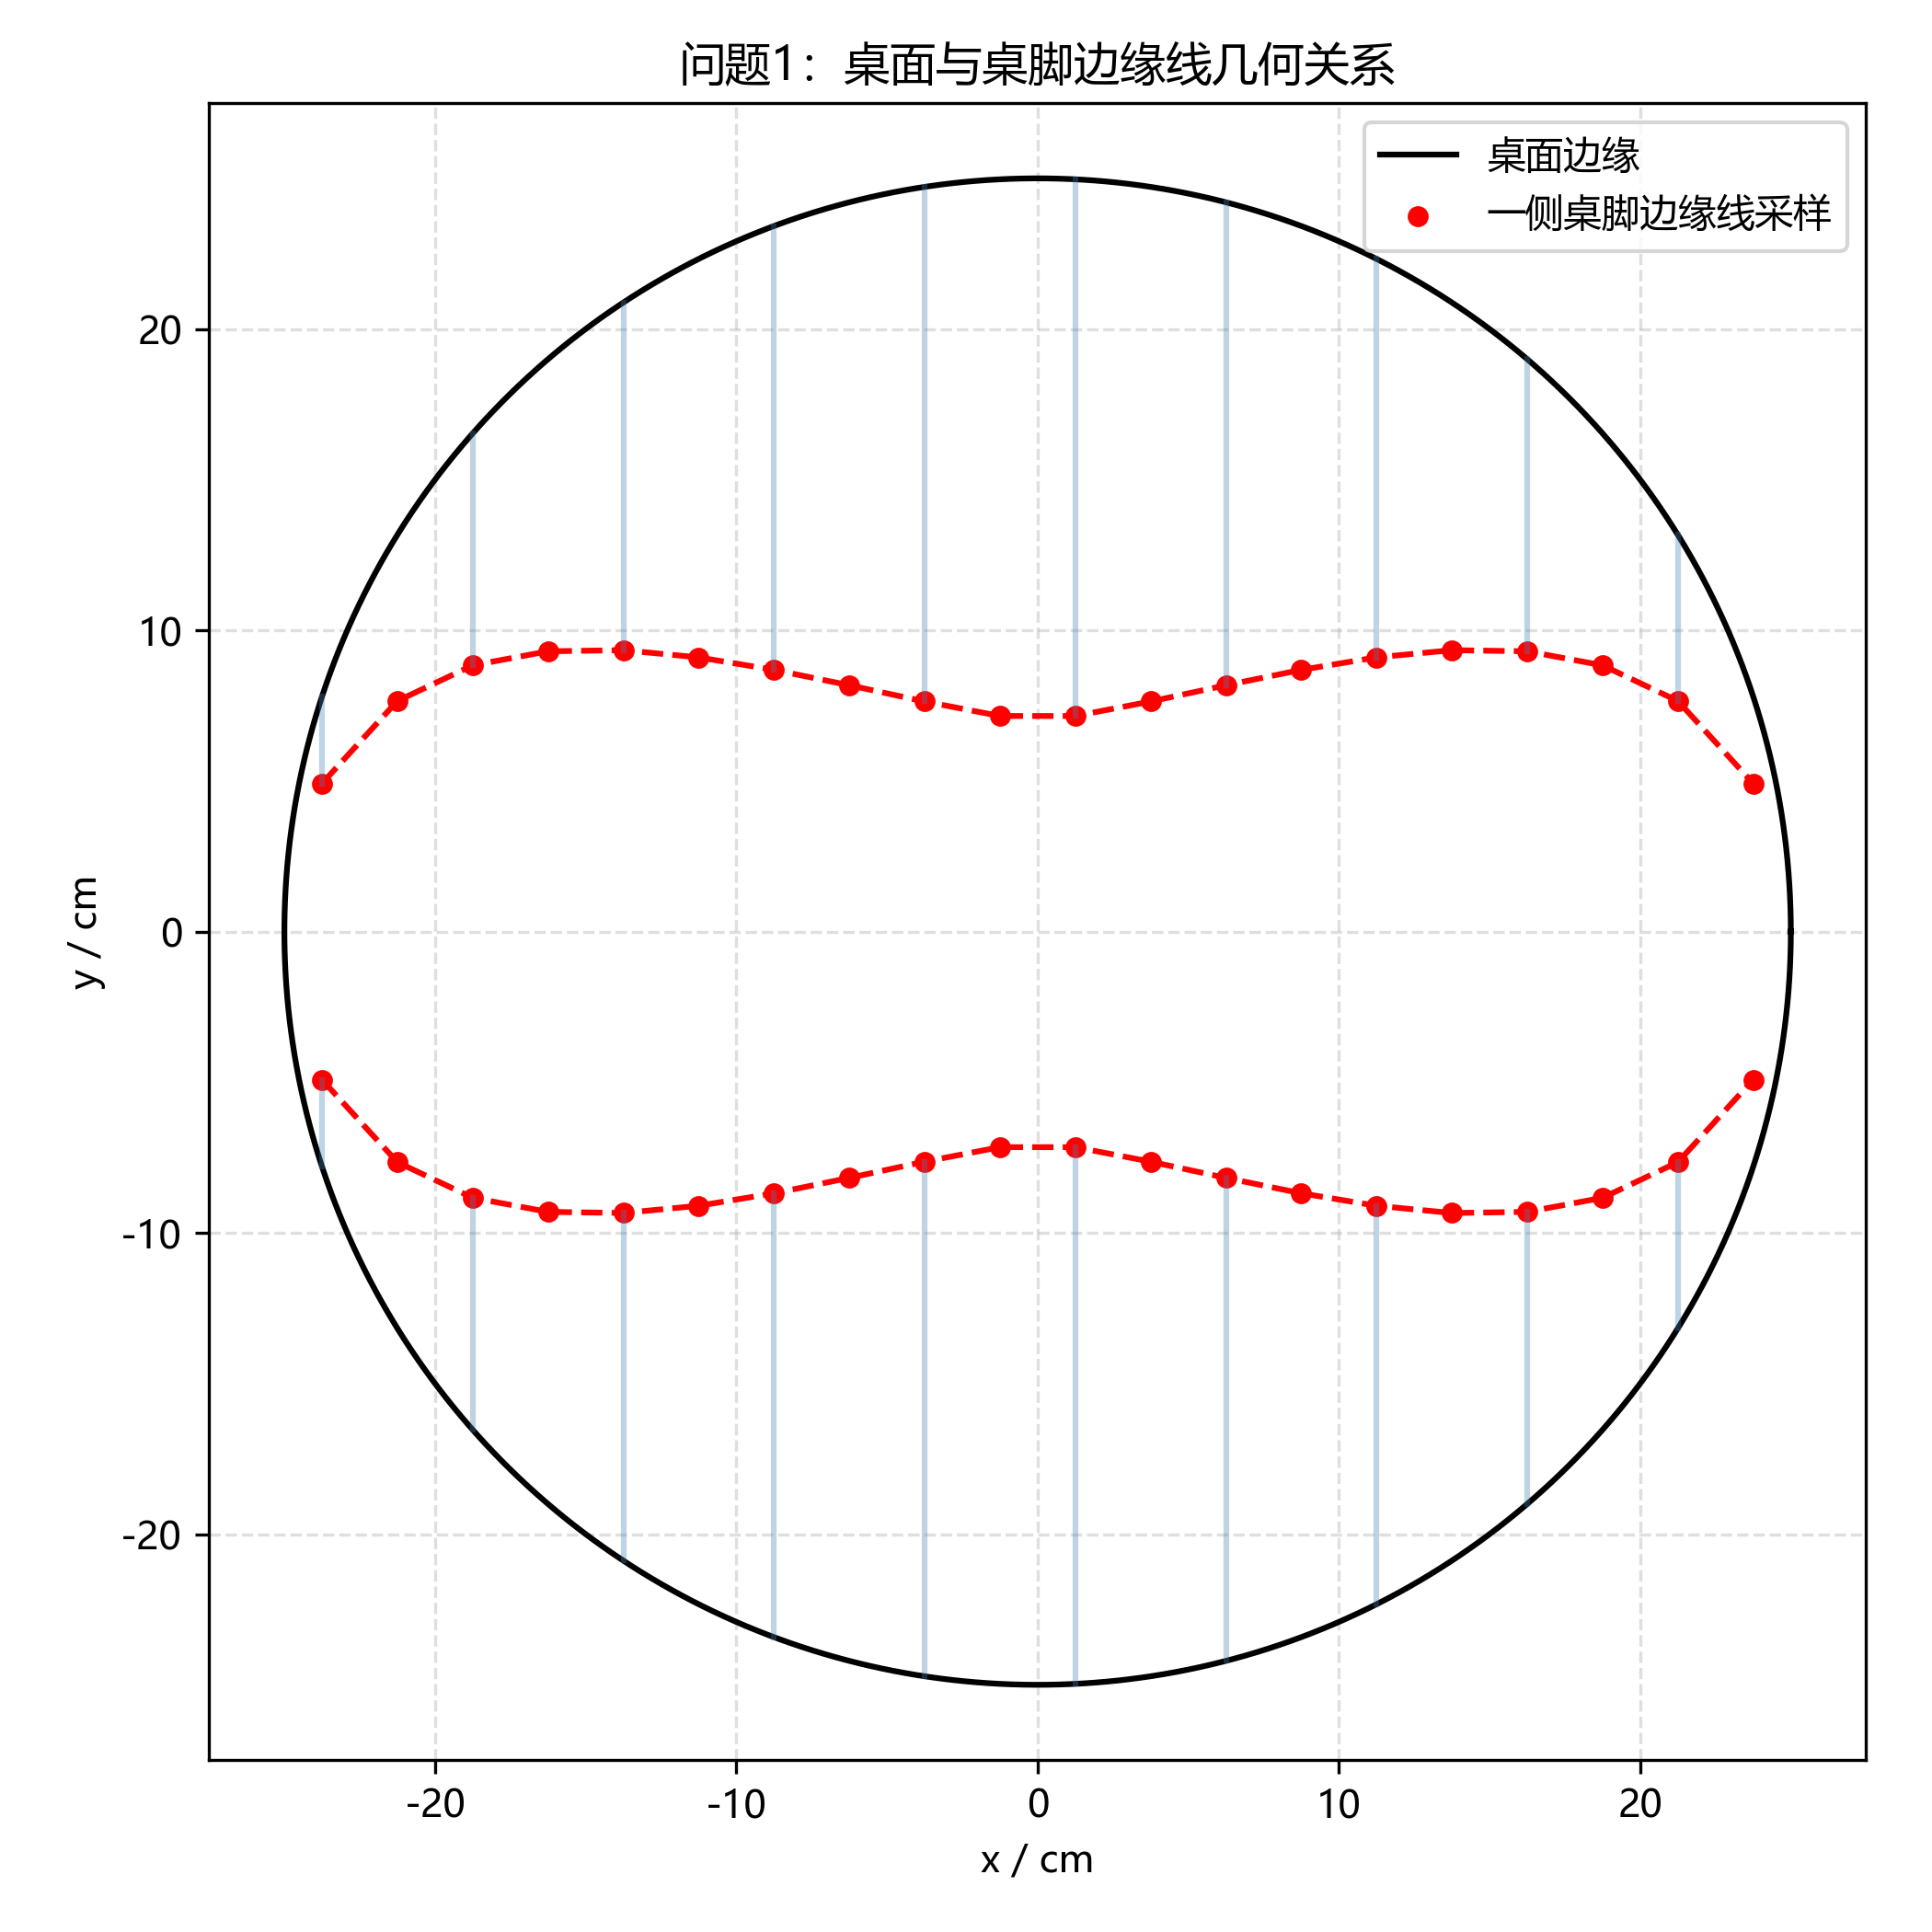
\includegraphics[width=0.72\textwidth]{q1_foot_curve.png}
\caption{问题一桌面边缘与桌脚边缘线}
\label{fig:q1foot}
\end{figure}
图\ref{fig:q1foot}显示了圆形桌面边界和桌脚边缘的关系。红色虚线为桌脚边缘采样曲线，整体位于圆桌面投影内部，说明桌脚不会外扩超过桌面范围。两侧木条保留较大支撑半径，中心木条适度内收，使外形呈现直纹曲面带来的弧线美感。

\begin{figure}[H]
\centering
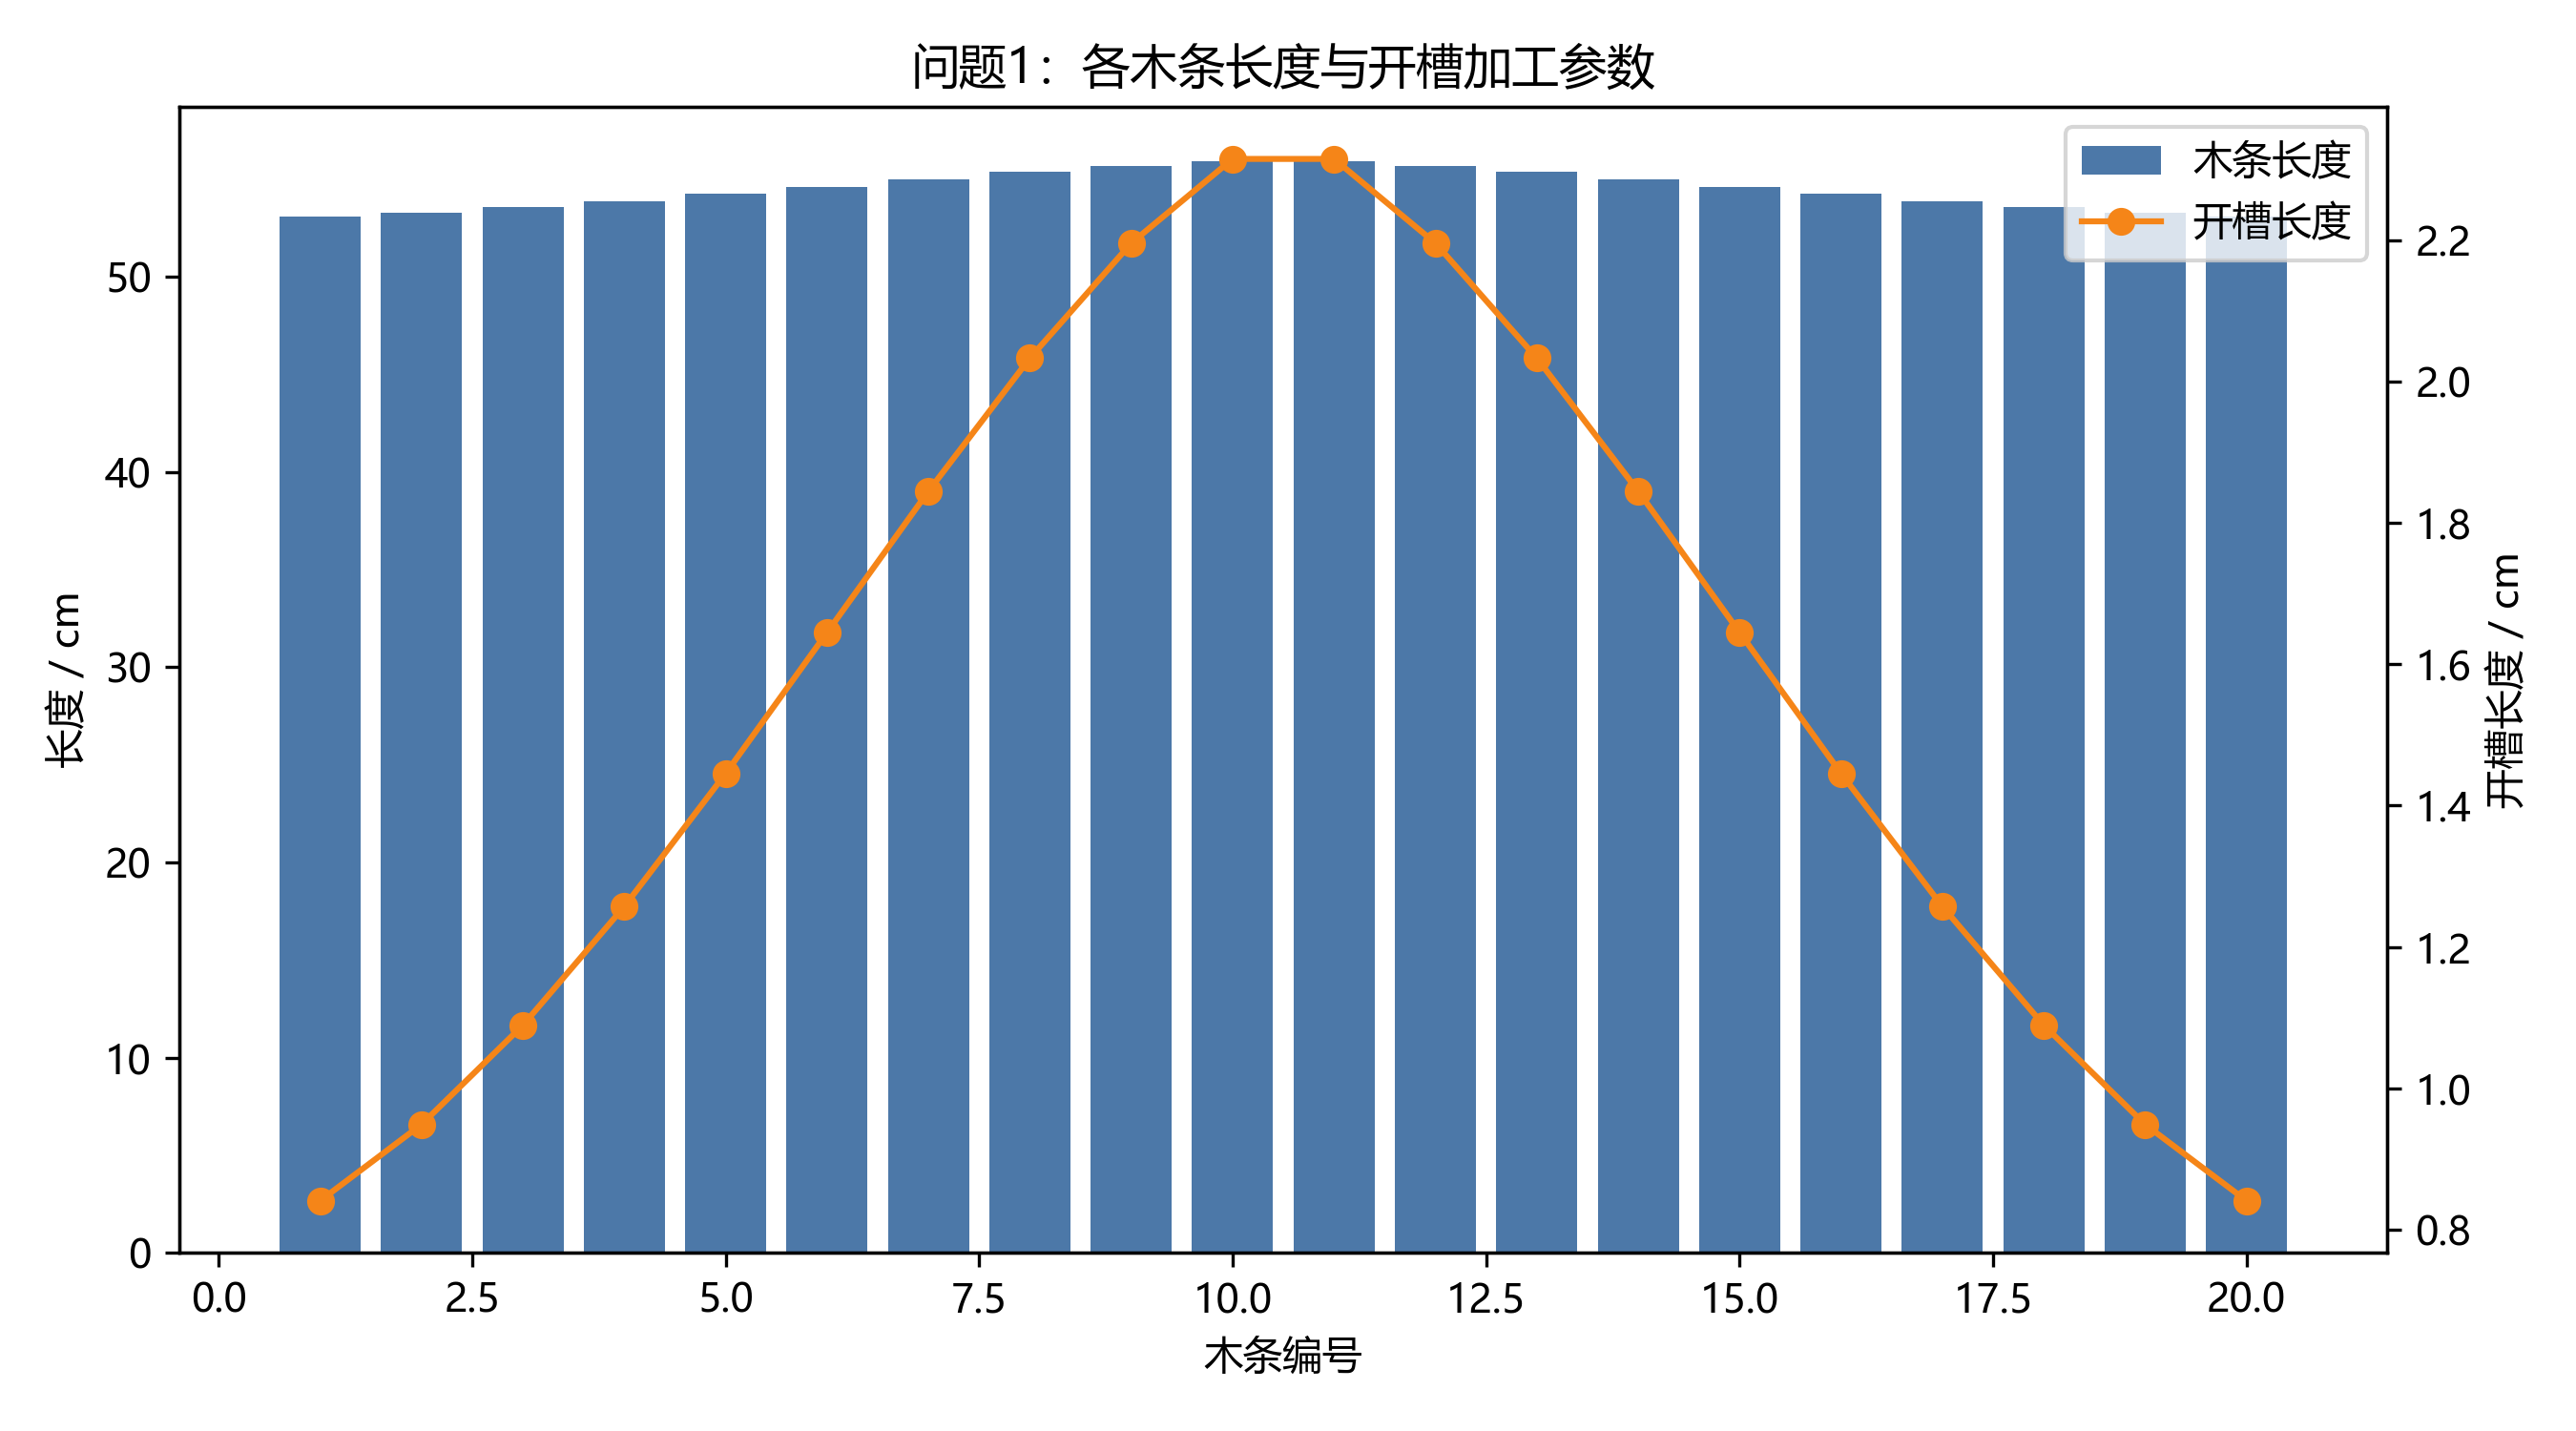
\includegraphics[width=0.82\textwidth]{q1_parameters.png}
\caption{问题一各木条长度和开槽长度}
\label{fig:q1param}
\end{figure}
图\ref{fig:q1param}表明，木条长度沿编号呈现对称分布，中间木条较短，两侧木条较长；开槽长度也呈对称变化。这与几何结构一致：靠近两侧的木条水平位移较大，需要更长木条和略长滑槽。图中不存在突变，说明该设计便于批量加工。

\begin{figure}[H]
\centering
\begin{subfigure}{0.31\textwidth}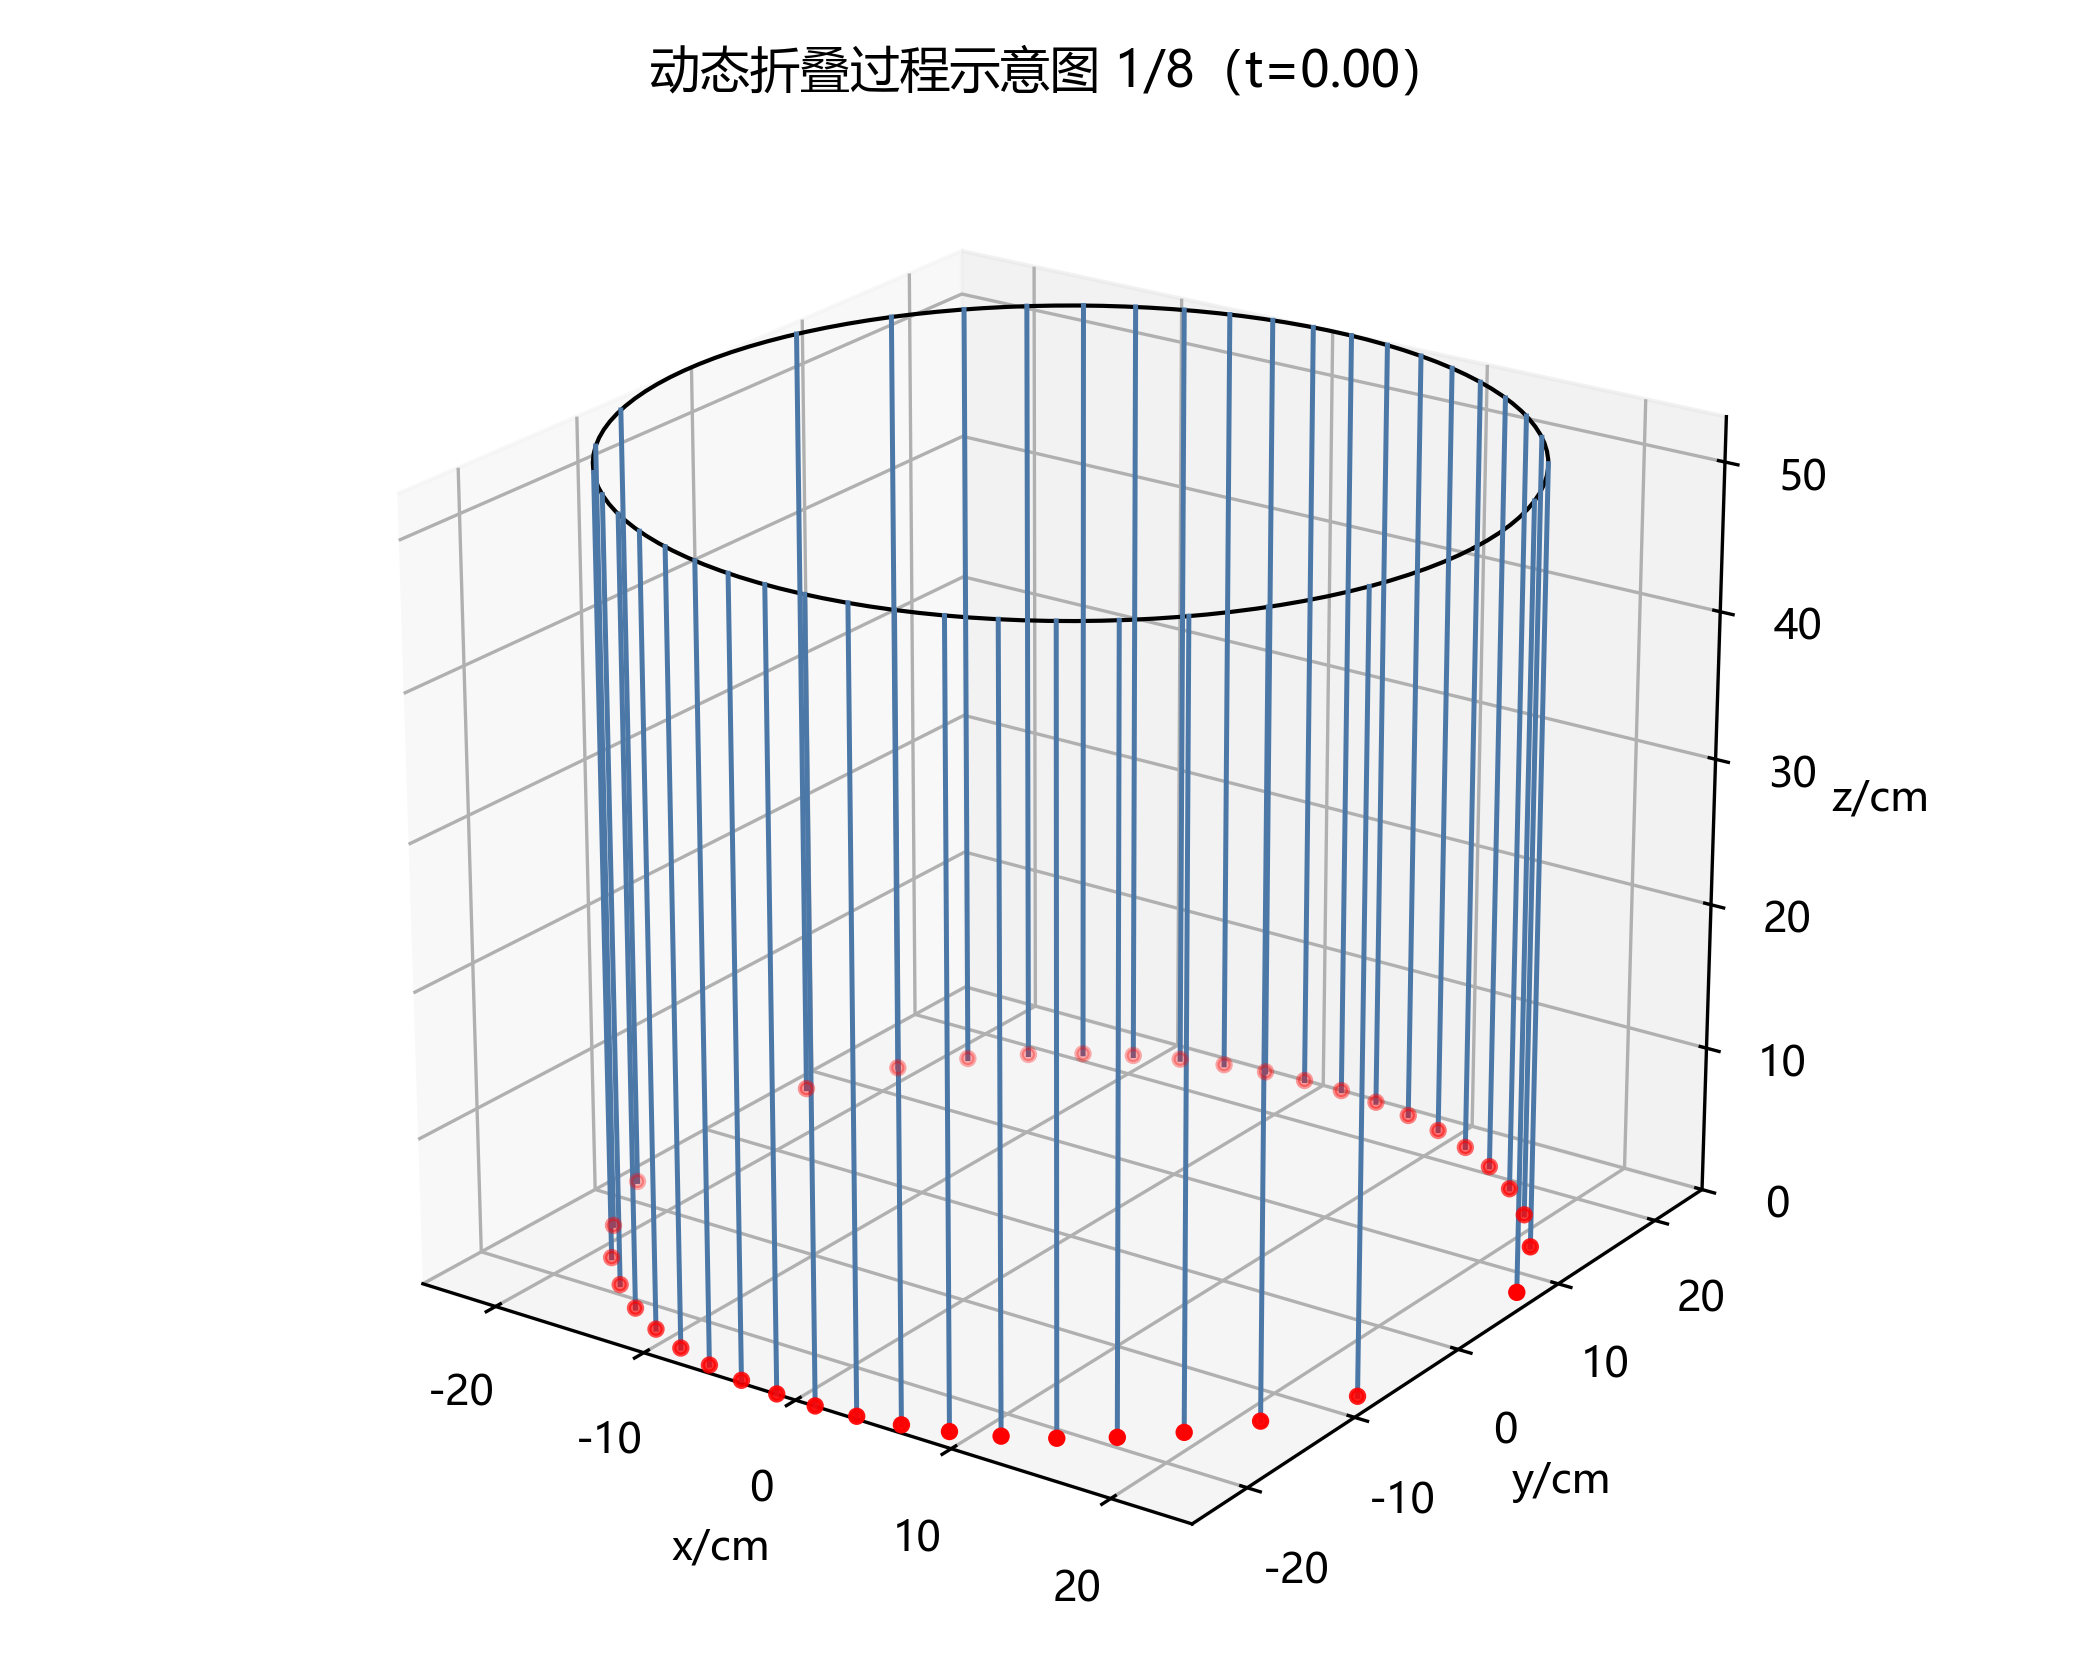
\includegraphics[width=\textwidth]{q1_dynamic_01.png}\caption{$t=0$}\end{subfigure}
\begin{subfigure}{0.31\textwidth}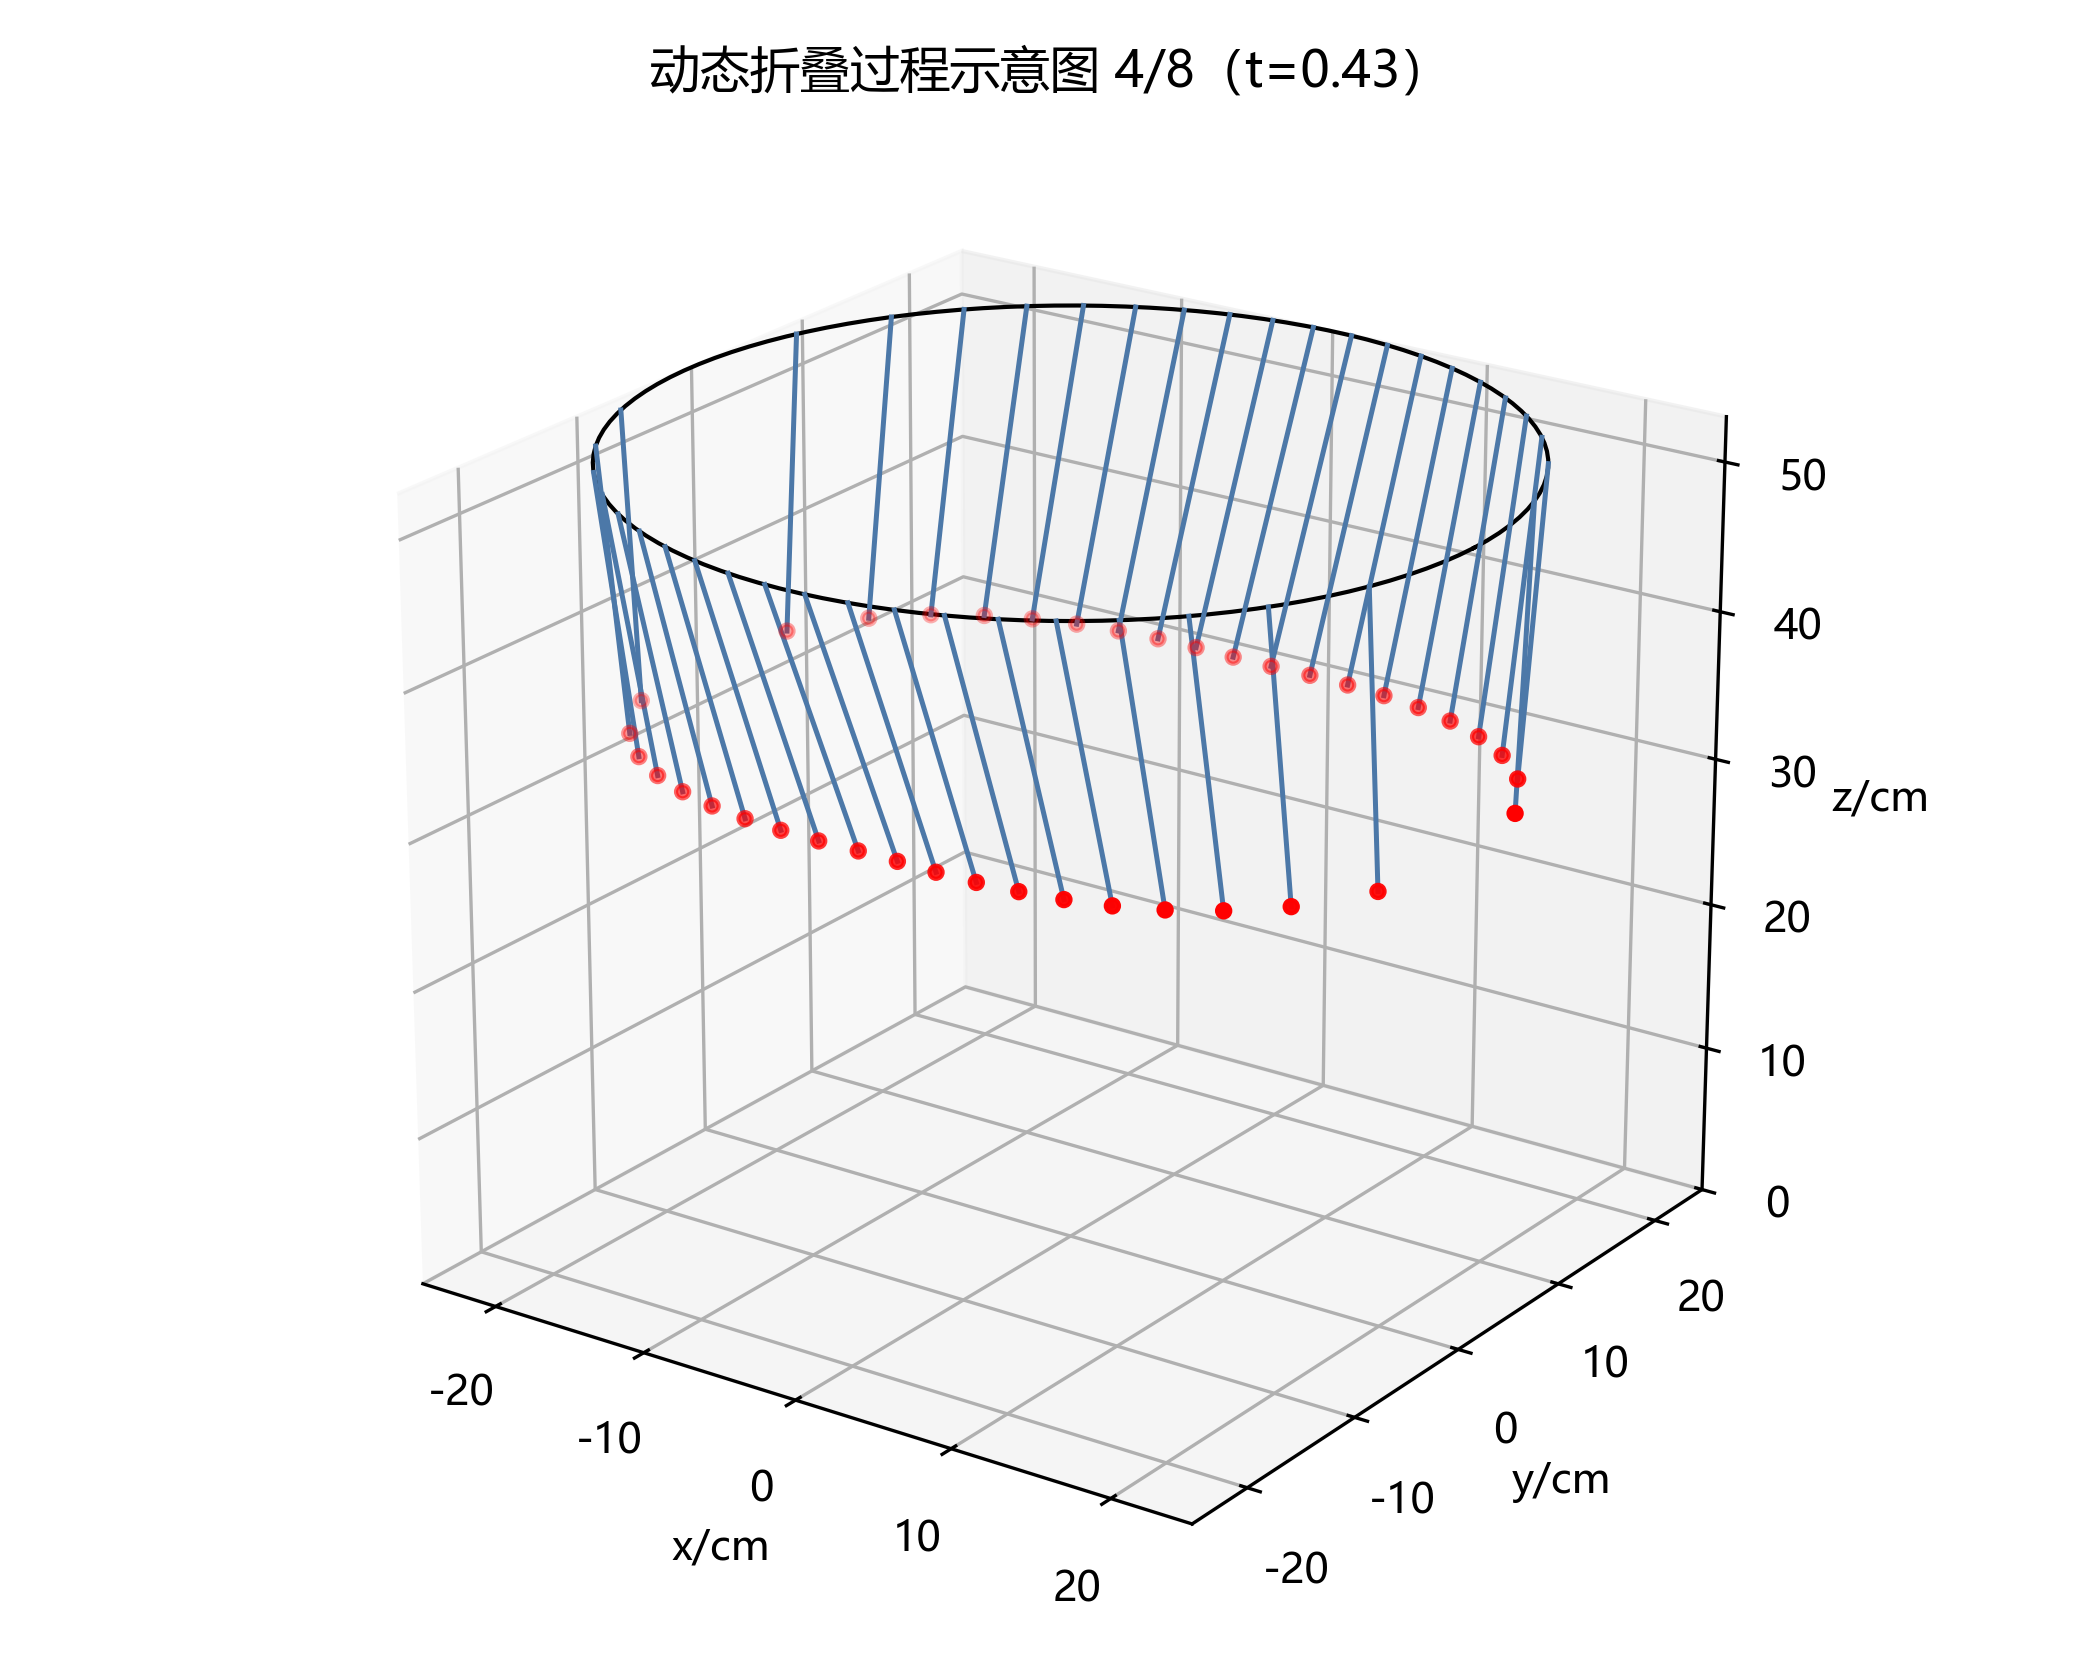
\includegraphics[width=\textwidth]{q1_dynamic_04.png}\caption{$t\approx0.43$}\end{subfigure}
\begin{subfigure}{0.31\textwidth}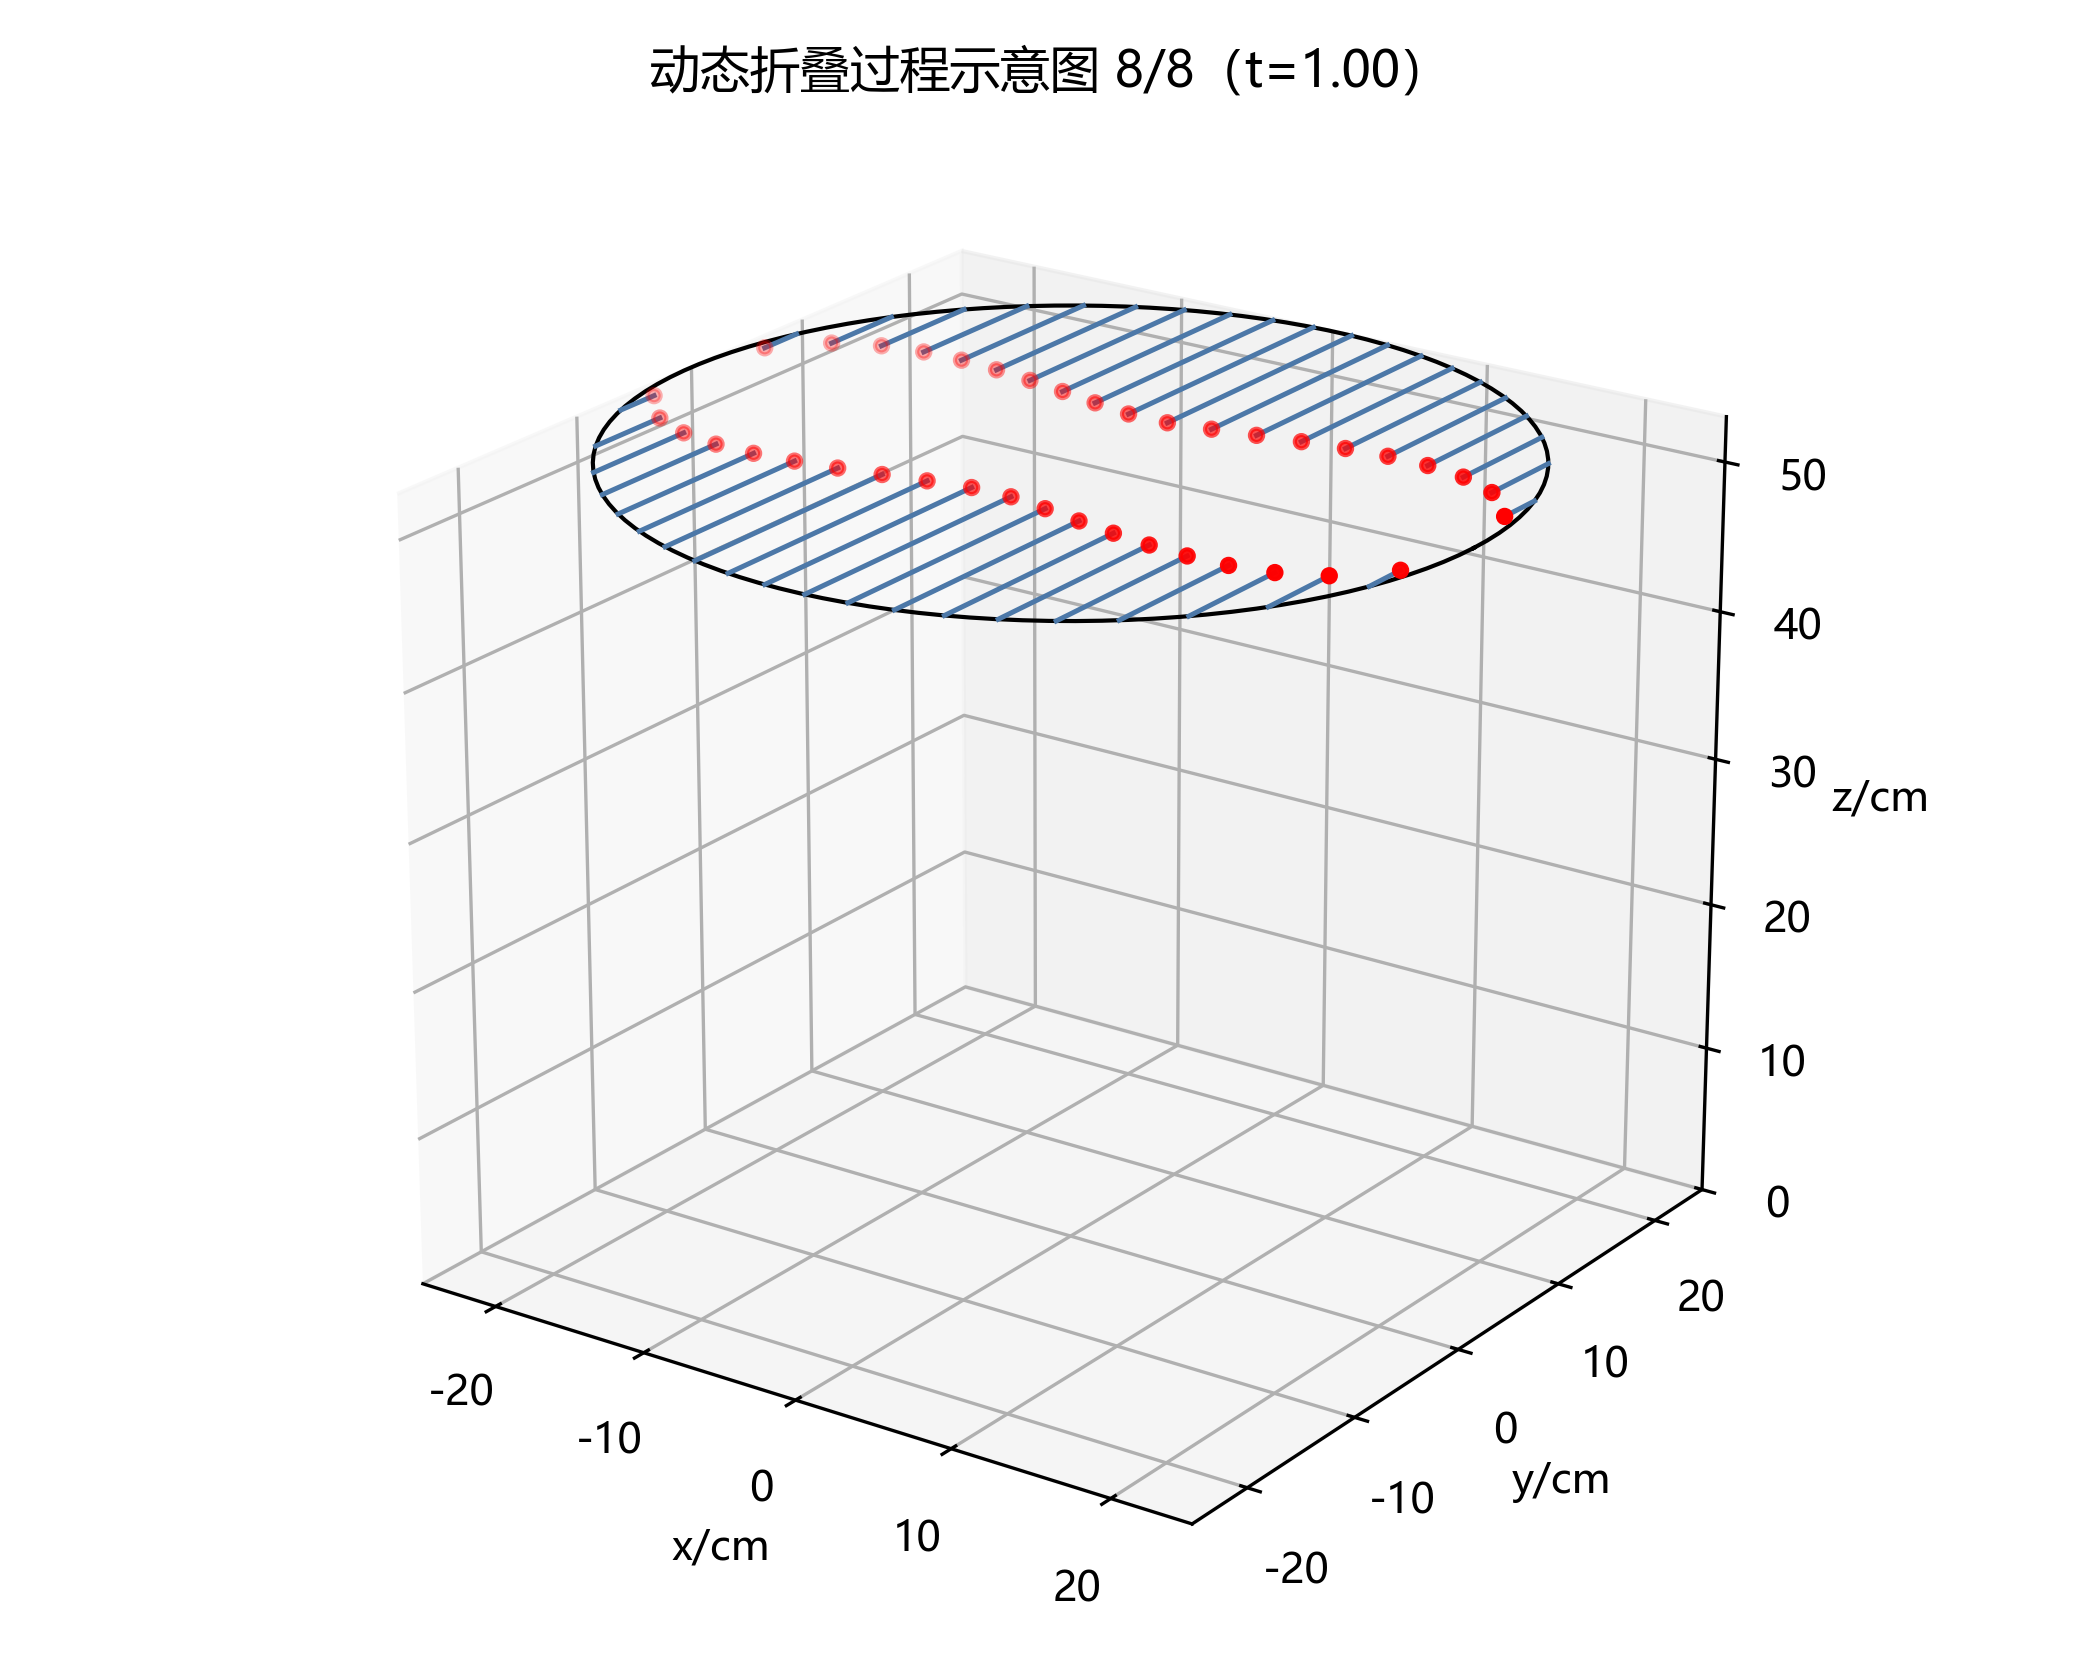
\includegraphics[width=\textwidth]{q1_dynamic_08.png}\caption{$t=1$}\end{subfigure}
\caption{问题一折叠过程中的三个代表时刻}
\label{fig:q1dyn}
\end{figure}
图\ref{fig:q1dyn}给出了动态过程中的三个代表状态。从左到右，桌腿由平摊逐步竖起，最终形成左右对称的空间支撑结构。由于每根木条均按同一折叠参数变化，整体外形在变化过程中保持连续，没有出现木条交叉或明显不协调的突变。

\subsection{问题二：任意桌高和直径下的优化设计}
\subsubsection{题目要求与模型输出对齐}
问题二要求：对任意给定桌高和圆桌面直径，讨论平板材料和设计加工参数的最优选择，并对 $H=70\cm,D=80\cm$ 给出数值方案。本文模型输出平板尺寸、木条数、钢筋相对位置、各木条长度、开槽长度，以及稳定性、加工性和材料效率指标。

\subsubsection{优化变量与约束}
对于给定 $D,H,w$，取优化变量为
\begin{equation}
 \boldsymbol{x}=(W,\eta),
\end{equation}
其中 $W$ 为平板宽度，$\eta$ 为钢筋孔距铰链端比例。木条数由
\begin{equation}
 N=\left\lfloor \frac{W}{w}\right\rfloor
\end{equation}
确定。为保证桌面完整，要求 $W\ge D$；为保证钢筋位置便于安装，取 $0.35\le\eta\le0.72$。此外要求支撑半径不低于桌面半径的55\%，最大倾角不超过 $38^\circ$，最大开槽长度不超过最大木条长度的18\%。这些约束分别对应稳定性、视觉造型和加工可行性。

\subsubsection{综合目标函数}
材料面积为
\begin{equation}
 A_m=2\max_i l_i\cdot W.
\end{equation}
稳定性指标定义为
\begin{equation}
 Q_s=\frac{r_s}{R}\left(1-0.22\overline{\frac{s_i}{l_i}}\right)
\left(1-0.15\frac{\sigma(\alpha_i)}{\overline{\alpha_i}}\right),
\end{equation}
其中 $r_s=\max_i\sqrt{x_i^2+(y_i^f)^2}$ 为支撑半径。该指标越大，说明支撑范围越大、开槽相对长度越短、倾角越均匀。

加工便利性指标定义为
\begin{equation}
 Q_p=\frac{1}{1+0.04\sigma(s_i)+0.015\max_i s_i+0.0008N}.
\end{equation}
若开槽长度差异大、最大开槽长或木条数过多，则加工便利性下降。综合目标函数取
\begin{equation}
 \min F=0.58\frac{A_m}{2.1DH}-0.28Q_s-0.14Q_p+P,
\end{equation}
其中 $P$ 为违反稳定半径、倾角和开槽约束的惩罚项。权重设置体现“用材最少”为主，同时保留稳定和加工要求。

\subsubsection{求解算法}
本文采用差分进化算法搜索 $(W,\eta)$。差分进化适合处理含整数木条数变化的非光滑目标函数，且不需要目标函数可导。算法步骤为：
\begin{enumerate}
\item 在 $W\in[D,D+35]$、$\eta\in[0.35,0.72]$ 范围内初始化种群；
\item 对每个候选方案计算木条数、长度、开槽长度、稳定性和加工性；
\item 对违反约束的方案加入惩罚；
\item 迭代变异、交叉和选择，直到目标函数收敛；
\item 对最优解进行局部抛光并输出最终加工参数。
\end{enumerate}
程序固定随机种子42，保证重复运行得到相同结论。

\subsubsection{实例结果：桌高70 cm、桌面直径80 cm}
优化结果如表\ref{tab:q2summary}所示。
\begin{table}[H]
\centering
\caption{$H=70\cm,D=80\cm$ 的优化设计参数}
\label{tab:q2summary}
\begin{tabular}{lcc}
\toprule
指标 & 数值 & 说明\\
\midrule
最优平板尺寸 & $151.272\times80.000\times3$ & cm\\
木条数 & 32 & $80/2.5=32$\\
钢筋位置比例 $\eta$ & 0.3500 & 距铰链端比例\\
木条长度范围 & $70.096$--$75.636$ & cm\\
最大开槽长度 & 2.773 & cm\\
平均开槽长度 & 1.793 & cm\\
支撑半径 & 39.251 & cm\\
稳定性指标 & 0.9173 & --\\
材料利用率 & 0.4154 & 圆桌面面积/平板面积\\
加工便利性 & 0.9150 & --\\
\bottomrule
\end{tabular}
\end{table}

该方案的平板宽度正好为 $80\cm$，说明在满足圆桌面直径的前提下，继续增加宽度带来的稳定性收益不足以抵消材料面积增加。钢筋位置比例取下界0.3500，说明钢筋靠近铰链端可以显著缩短滑槽长度，提高加工便利性。最大开槽长度为 $2.773\cm$，只占最大木条长度约3.67\%，属于容易加工的范围。

\begin{figure}[H]
\centering
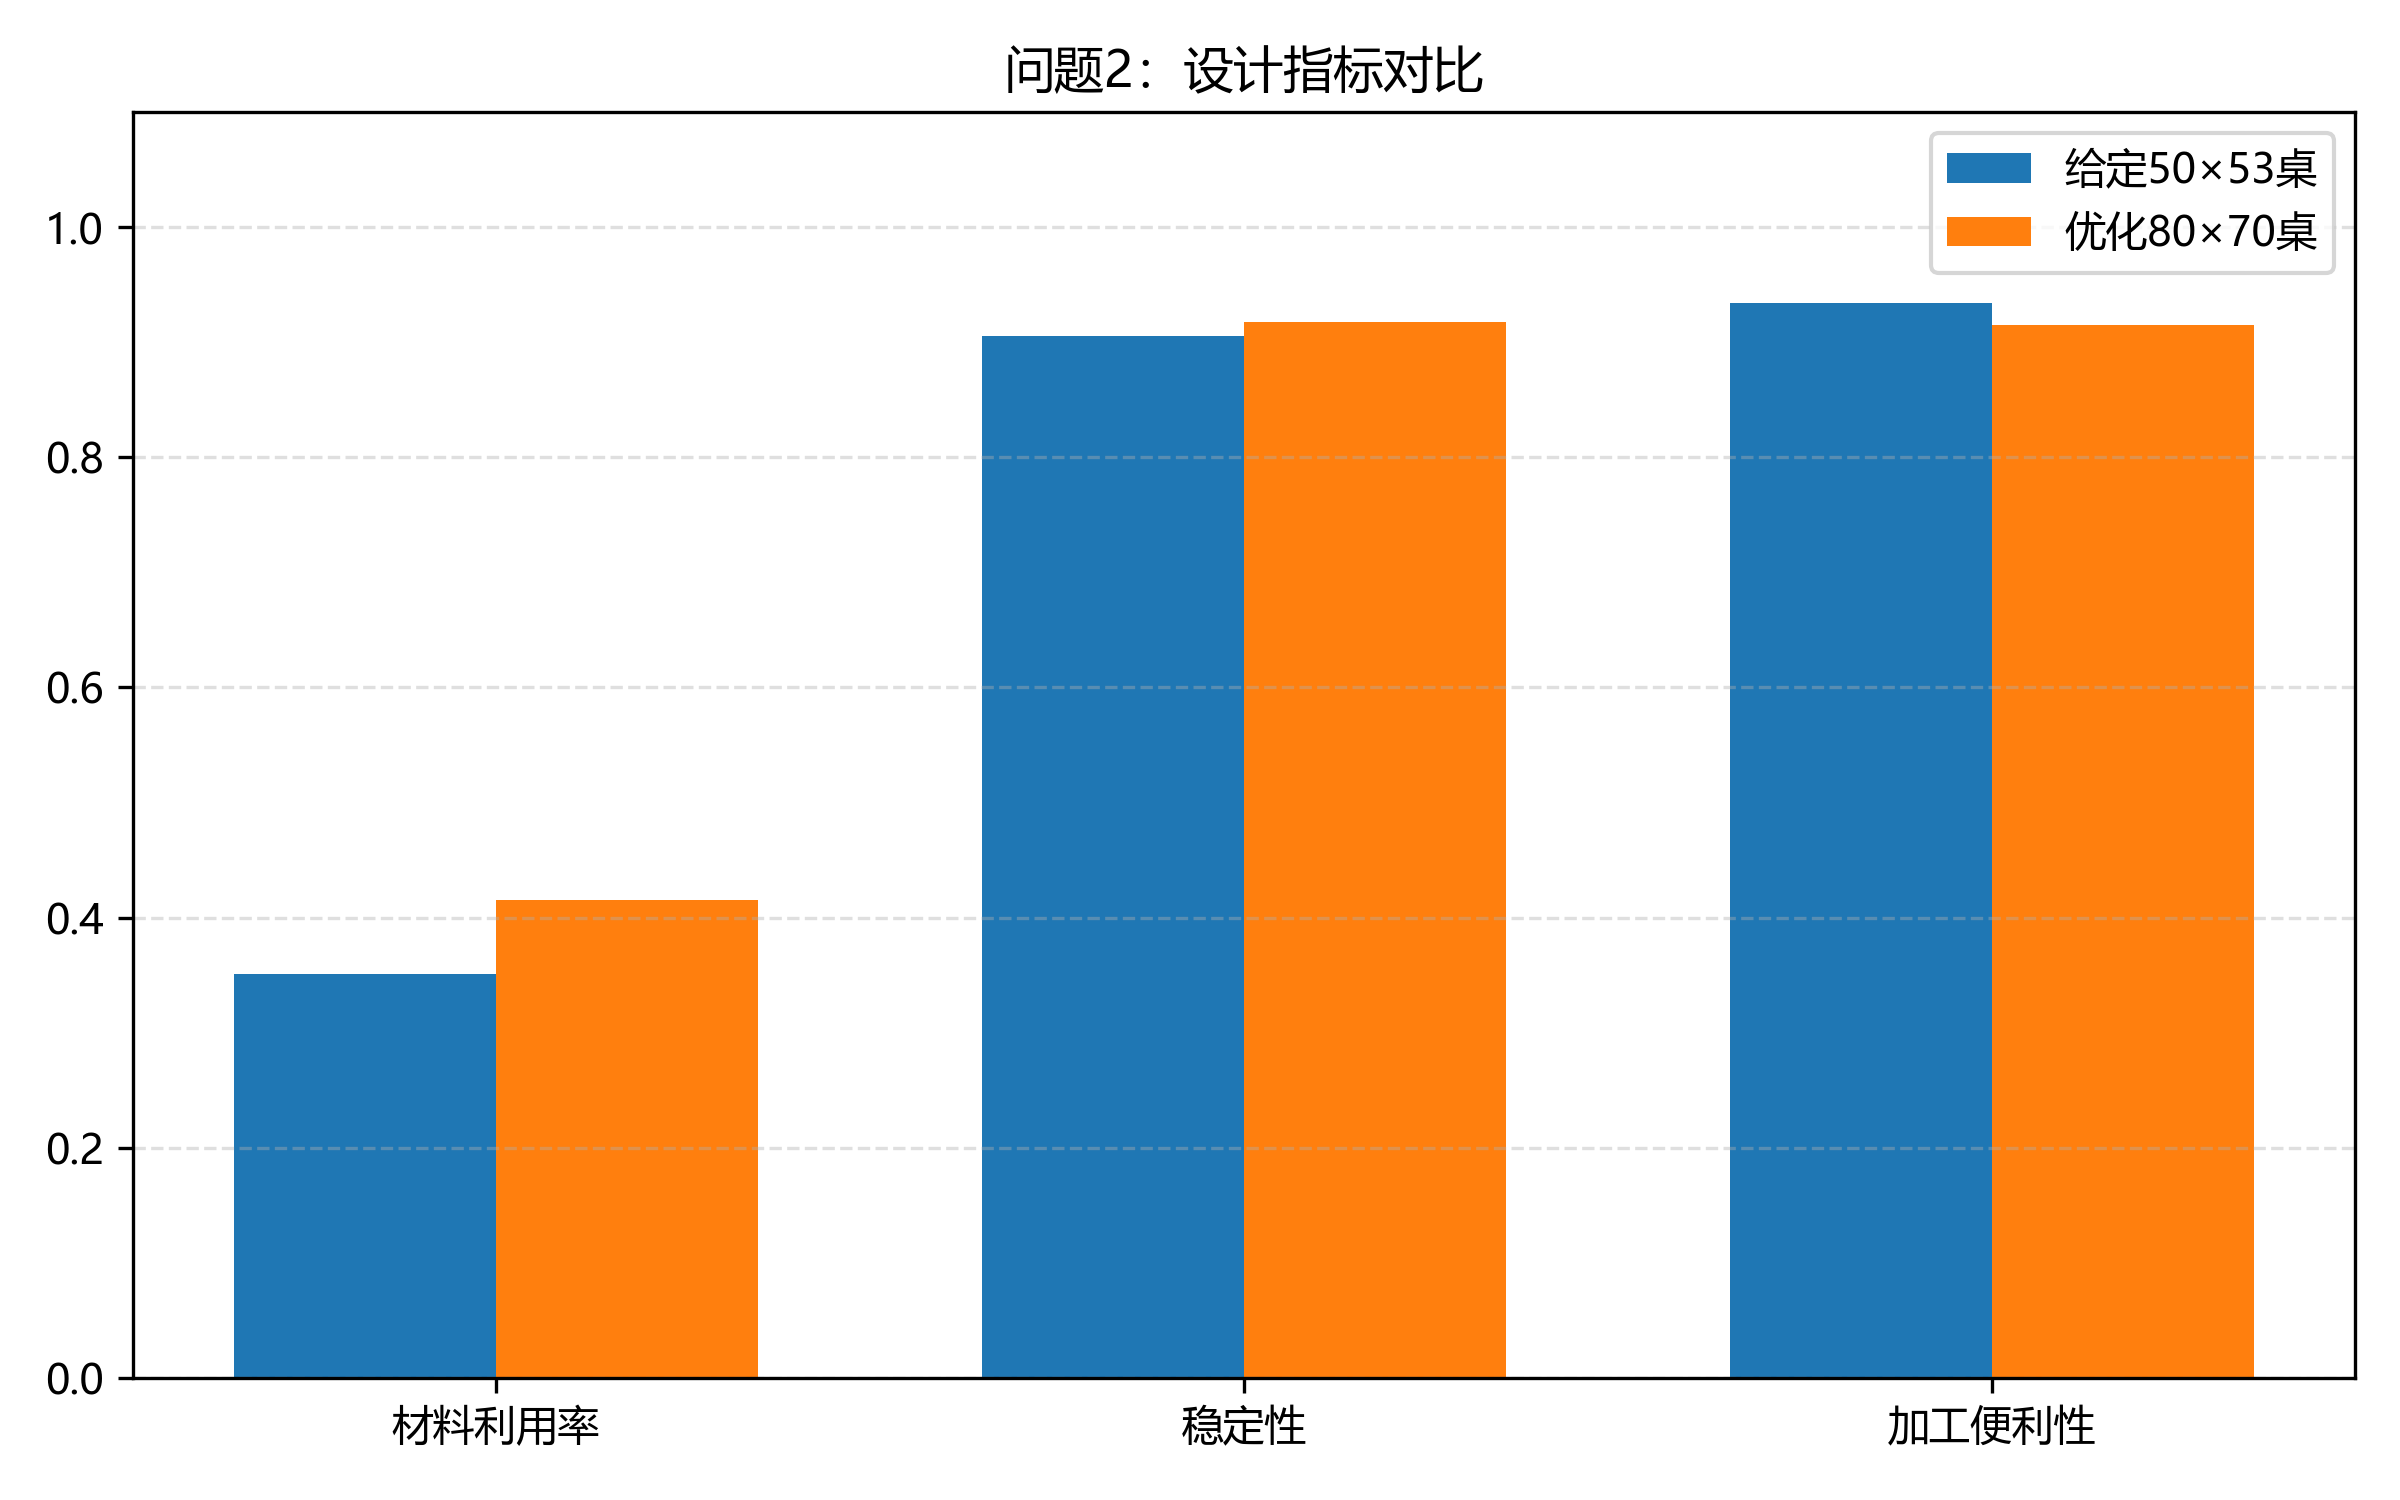
\includegraphics[width=0.78\textwidth]{q2_design_metrics.png}
\caption{问题二优化方案与问题一方案的设计指标对比}
\label{fig:q2metrics}
\end{figure}
图\ref{fig:q2metrics}比较了材料利用率、稳定性和加工便利性。优化后的 $80\cm\times70\cm$ 折叠桌由于桌面更大，材料利用率相对较低，但稳定性指标达到0.9173，高于问题一方案；加工便利性仍保持在0.9150左右，说明开槽长度和木条数量没有造成明显加工负担。

\subsubsection{baseline 对比}
问题二 baseline 方案取 $W=D=80\cm,\eta=0.5$，即钢筋位于木条中部。该方案的支撑半径和总体木条长度与优化方案接近，但最大开槽长度为 $3.618\cm$。优化方案通过将钢筋比例调至0.3500，将最大开槽长度降至 $2.773\cm$，降低约23.36\%。这说明主模型相对 baseline 的主要优势是减少加工难度，而不是单纯改变整体外形。

\subsection{问题三：面向设计软件的通用数学模型}
\subsubsection{题目要求与模型输出对齐}
问题三要求建立软件模型：客户给定桌高、桌面边缘形状大小和桌脚边缘大致形状，软件输出平板材料尺寸和可行加工参数，并尽可能接近期望形状。本文模型输出通用优化框架、三类创意折叠桌参数、三维成型图和8张动态变化图。

\subsubsection{通用边界离散模型}
设客户给定桌面边缘曲线为 $C_t$，期望桌脚边缘曲线为 $C_f^*$。在宽度方向离散点 $x_i$ 上，分别计算桌面半宽 $y_i^t$ 和期望桌脚半宽 $y_i^{f*}$。软件需寻找实际桌脚半宽 $y_i^f$、平板宽度 $W$ 和钢筋比例 $\eta$，使其满足
\begin{equation}
 0\le y_i^f\le y_i^t,\quad l_i=\sqrt{H^2+(y_i^t-y_i^f)^2},
\end{equation}
并使目标函数最小：
\begin{equation}
 \min J=\lambda_1\sum_i(y_i^f-y_i^{f*})^2+\lambda_2 A_m+\lambda_3\sum_i s_i^2-\lambda_4 Q_s.
\end{equation}
其中第一项衡量与客户期望桌脚线的接近程度，第二项控制用材，第三项控制开槽复杂度，第四项提高稳定性。约束包括木条长度上限、最大开槽长度、最小支撑半径和相邻木条长度差限制。

\subsubsection{软件流程设计}
本文建议软件采用以下流程：
\begin{enumerate}
\item 输入：桌高 $H$、桌面边界 $C_t$、期望桌脚边界 $C_f^*$、木条宽度 $w$ 和加工约束；
\item 离散：按木条宽度生成 $x_i$，计算每根木条对应的桌面边界坐标；
\item 初值：将期望桌脚边界投影到可行区域 $0\le y_i^f\le y_i^t$；
\item 优化：最小化边界误差、材料面积和开槽复杂度，并检查稳定性；
\item 输出：平板尺寸、木条编号表、开槽长度表、钢筋孔位、二维加工图和三维动态图；
\item 反馈：若用户对外形不满意，可调整权重 $\lambda_1$--$\lambda_4$ 重新优化。
\end{enumerate}

\subsubsection{创意折叠桌实例}
本文给出三种创意桌面：椭圆形、圆角方形和花瓣形。主要参数见表\ref{tab:q3summary}。
\begin{table}[H]
\centering
\caption{问题三创意折叠桌设计参数}
\label{tab:q3summary}
\begin{tabular}{lccc}
\toprule
设计名称 & 平板尺寸/cm & 木条数 & 最大开槽/cm\\
\midrule
椭圆桌 & $134.615\times90.000\times3$ & 36 & 2.000\\
圆角方形桌 & $131.836\times80.000\times3$ & 32 & 2.837\\
花瓣桌 & $140.917\times87.500\times3$ & 35 & 2.078\\
\bottomrule
\end{tabular}
\end{table}

椭圆桌适合长向空间布置，桌面横向尺度为 $90\cm$、纵向尺度为 $60\cm$；圆角方形桌保留方桌使用效率，同时通过圆角降低边缘突变；花瓣桌强调造型创意，桌脚边缘随桌面曲线产生柔和起伏。三类设计的最大开槽长度均小于 $3\cm$，说明模型能在不同外形下保持加工可行性。

\begin{figure}[H]
\centering
\begin{subfigure}{0.32\textwidth}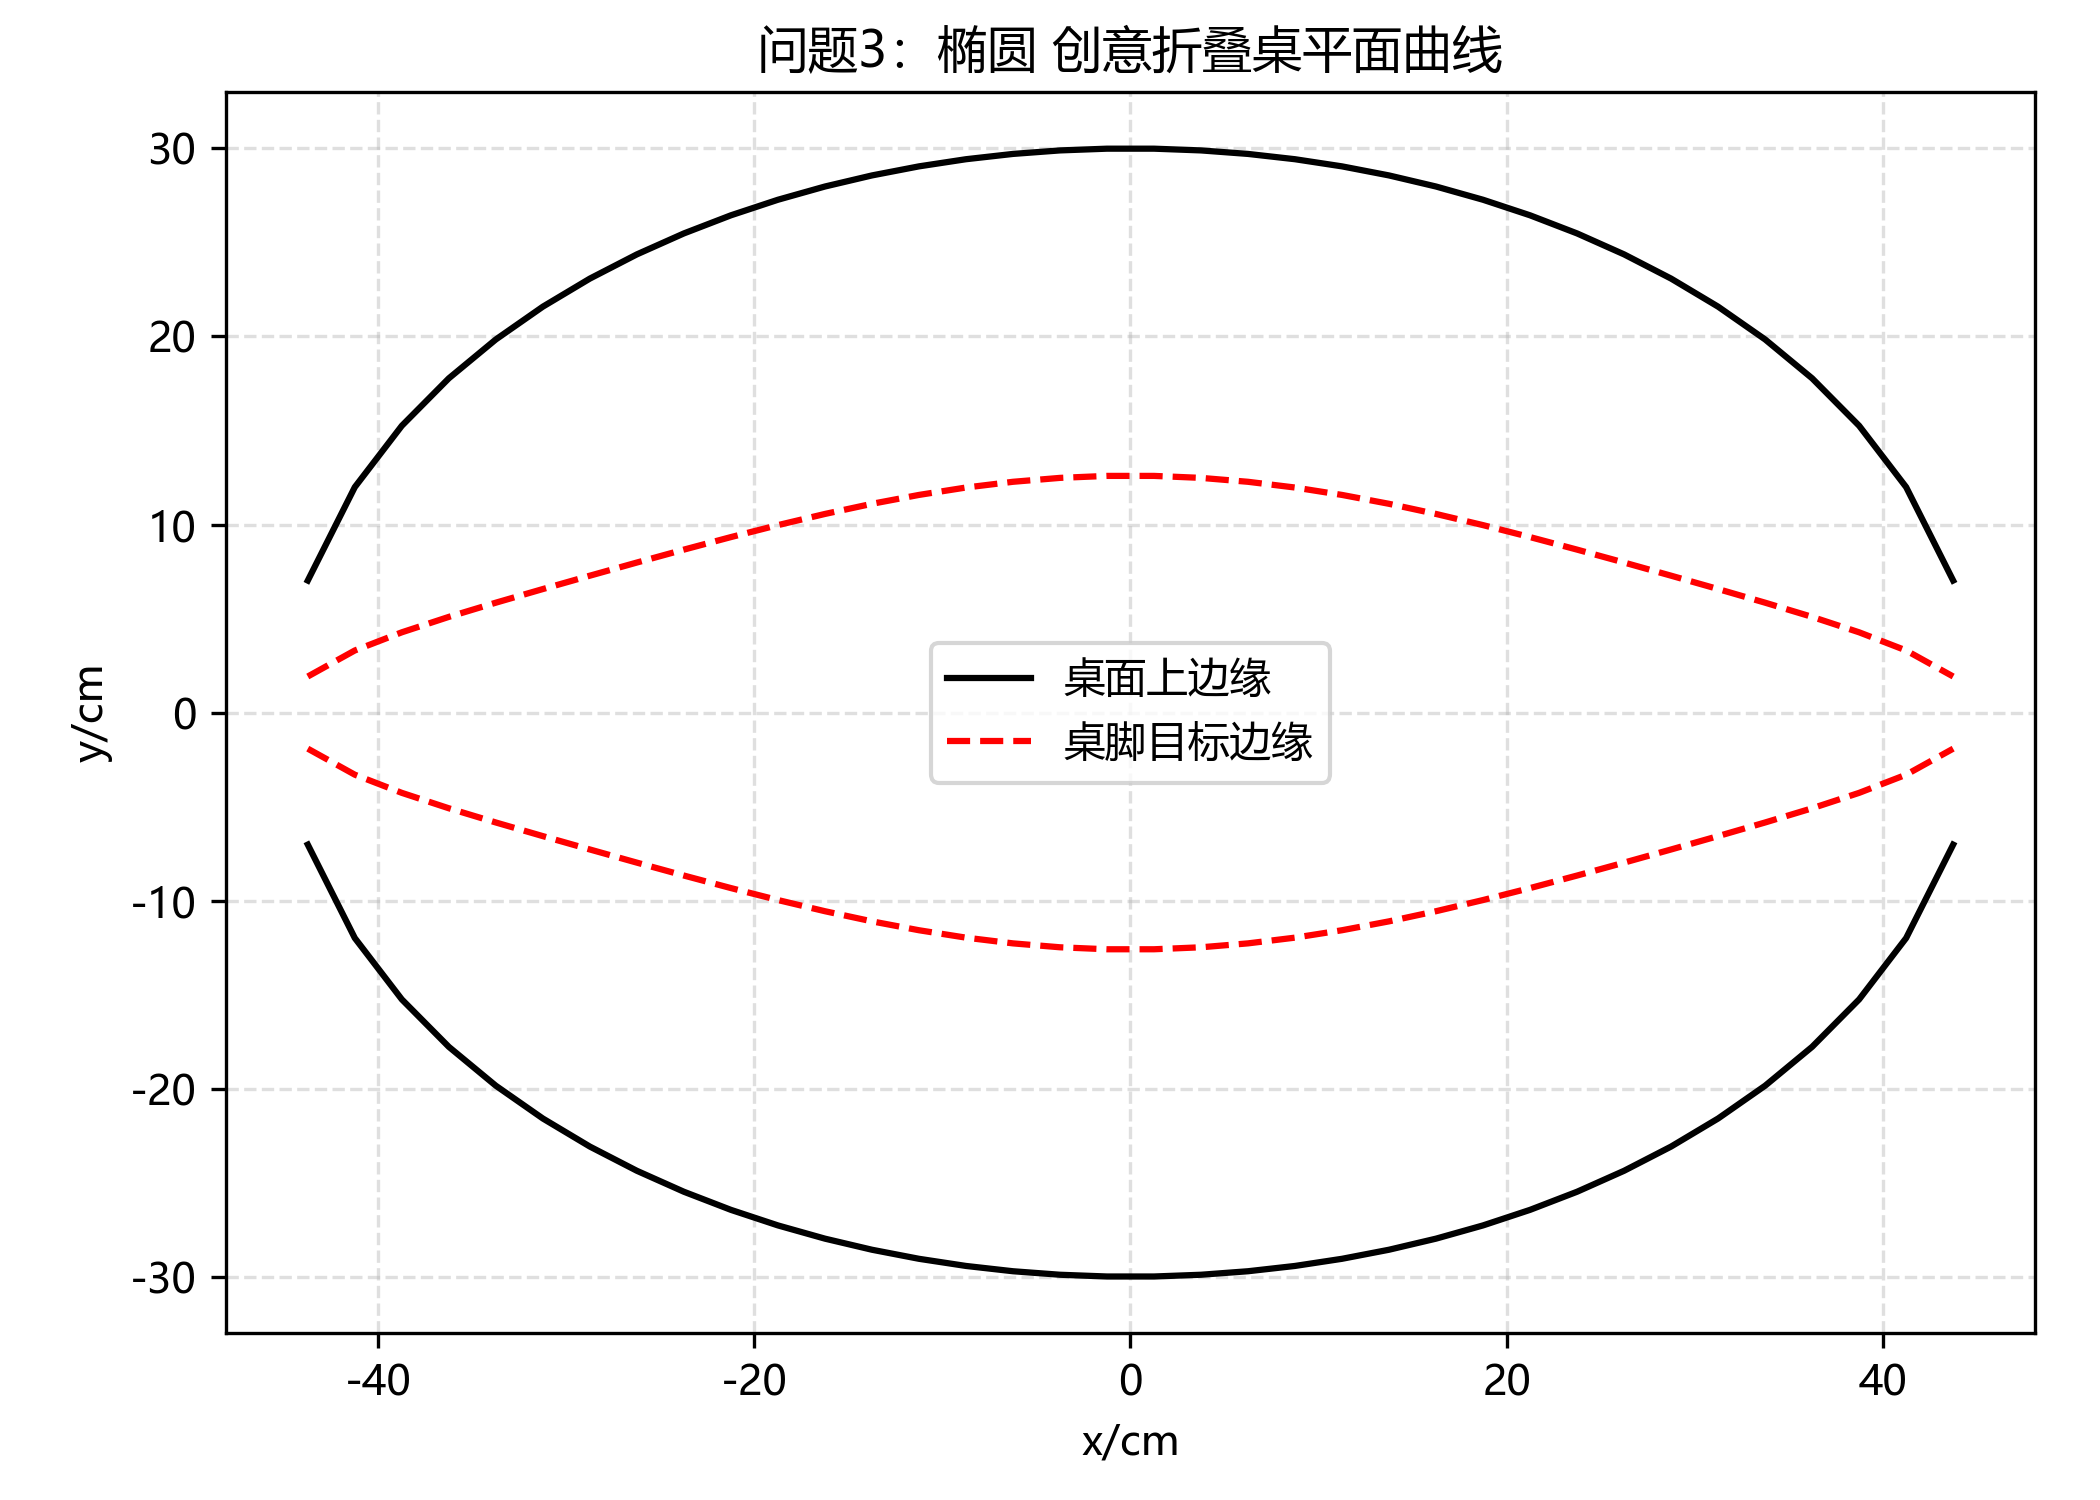
\includegraphics[width=\textwidth]{q3_ellipse_curves.png}\caption{椭圆}\end{subfigure}
\begin{subfigure}{0.32\textwidth}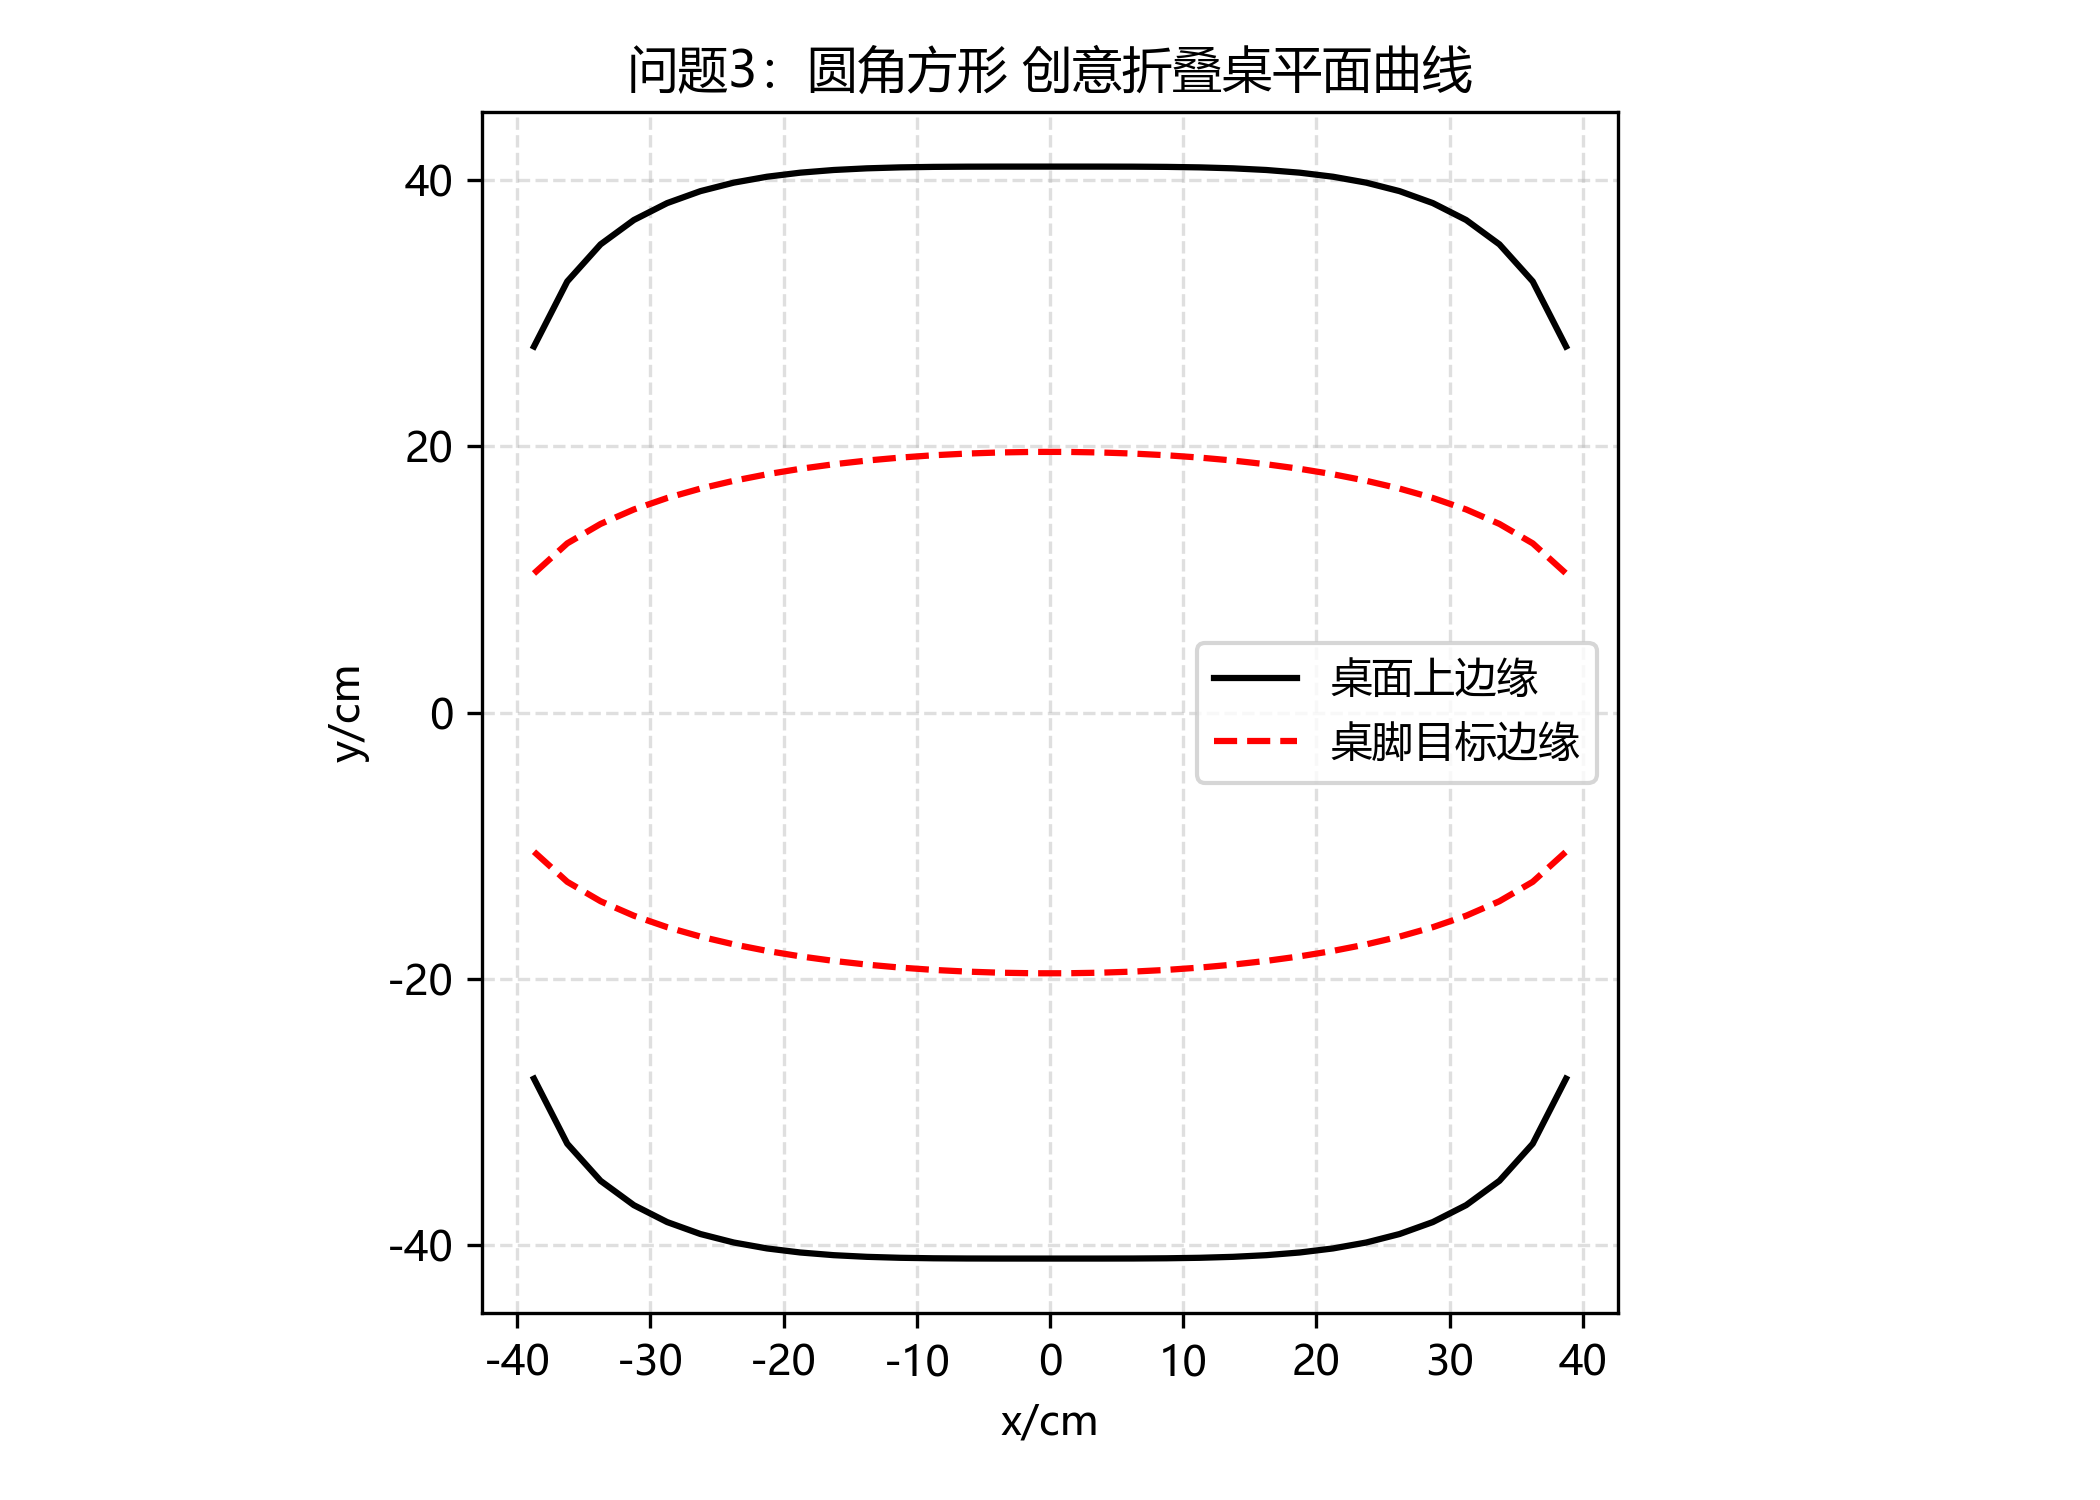
\includegraphics[width=\textwidth]{q3_rounded_square_curves.png}\caption{圆角方形}\end{subfigure}
\begin{subfigure}{0.32\textwidth}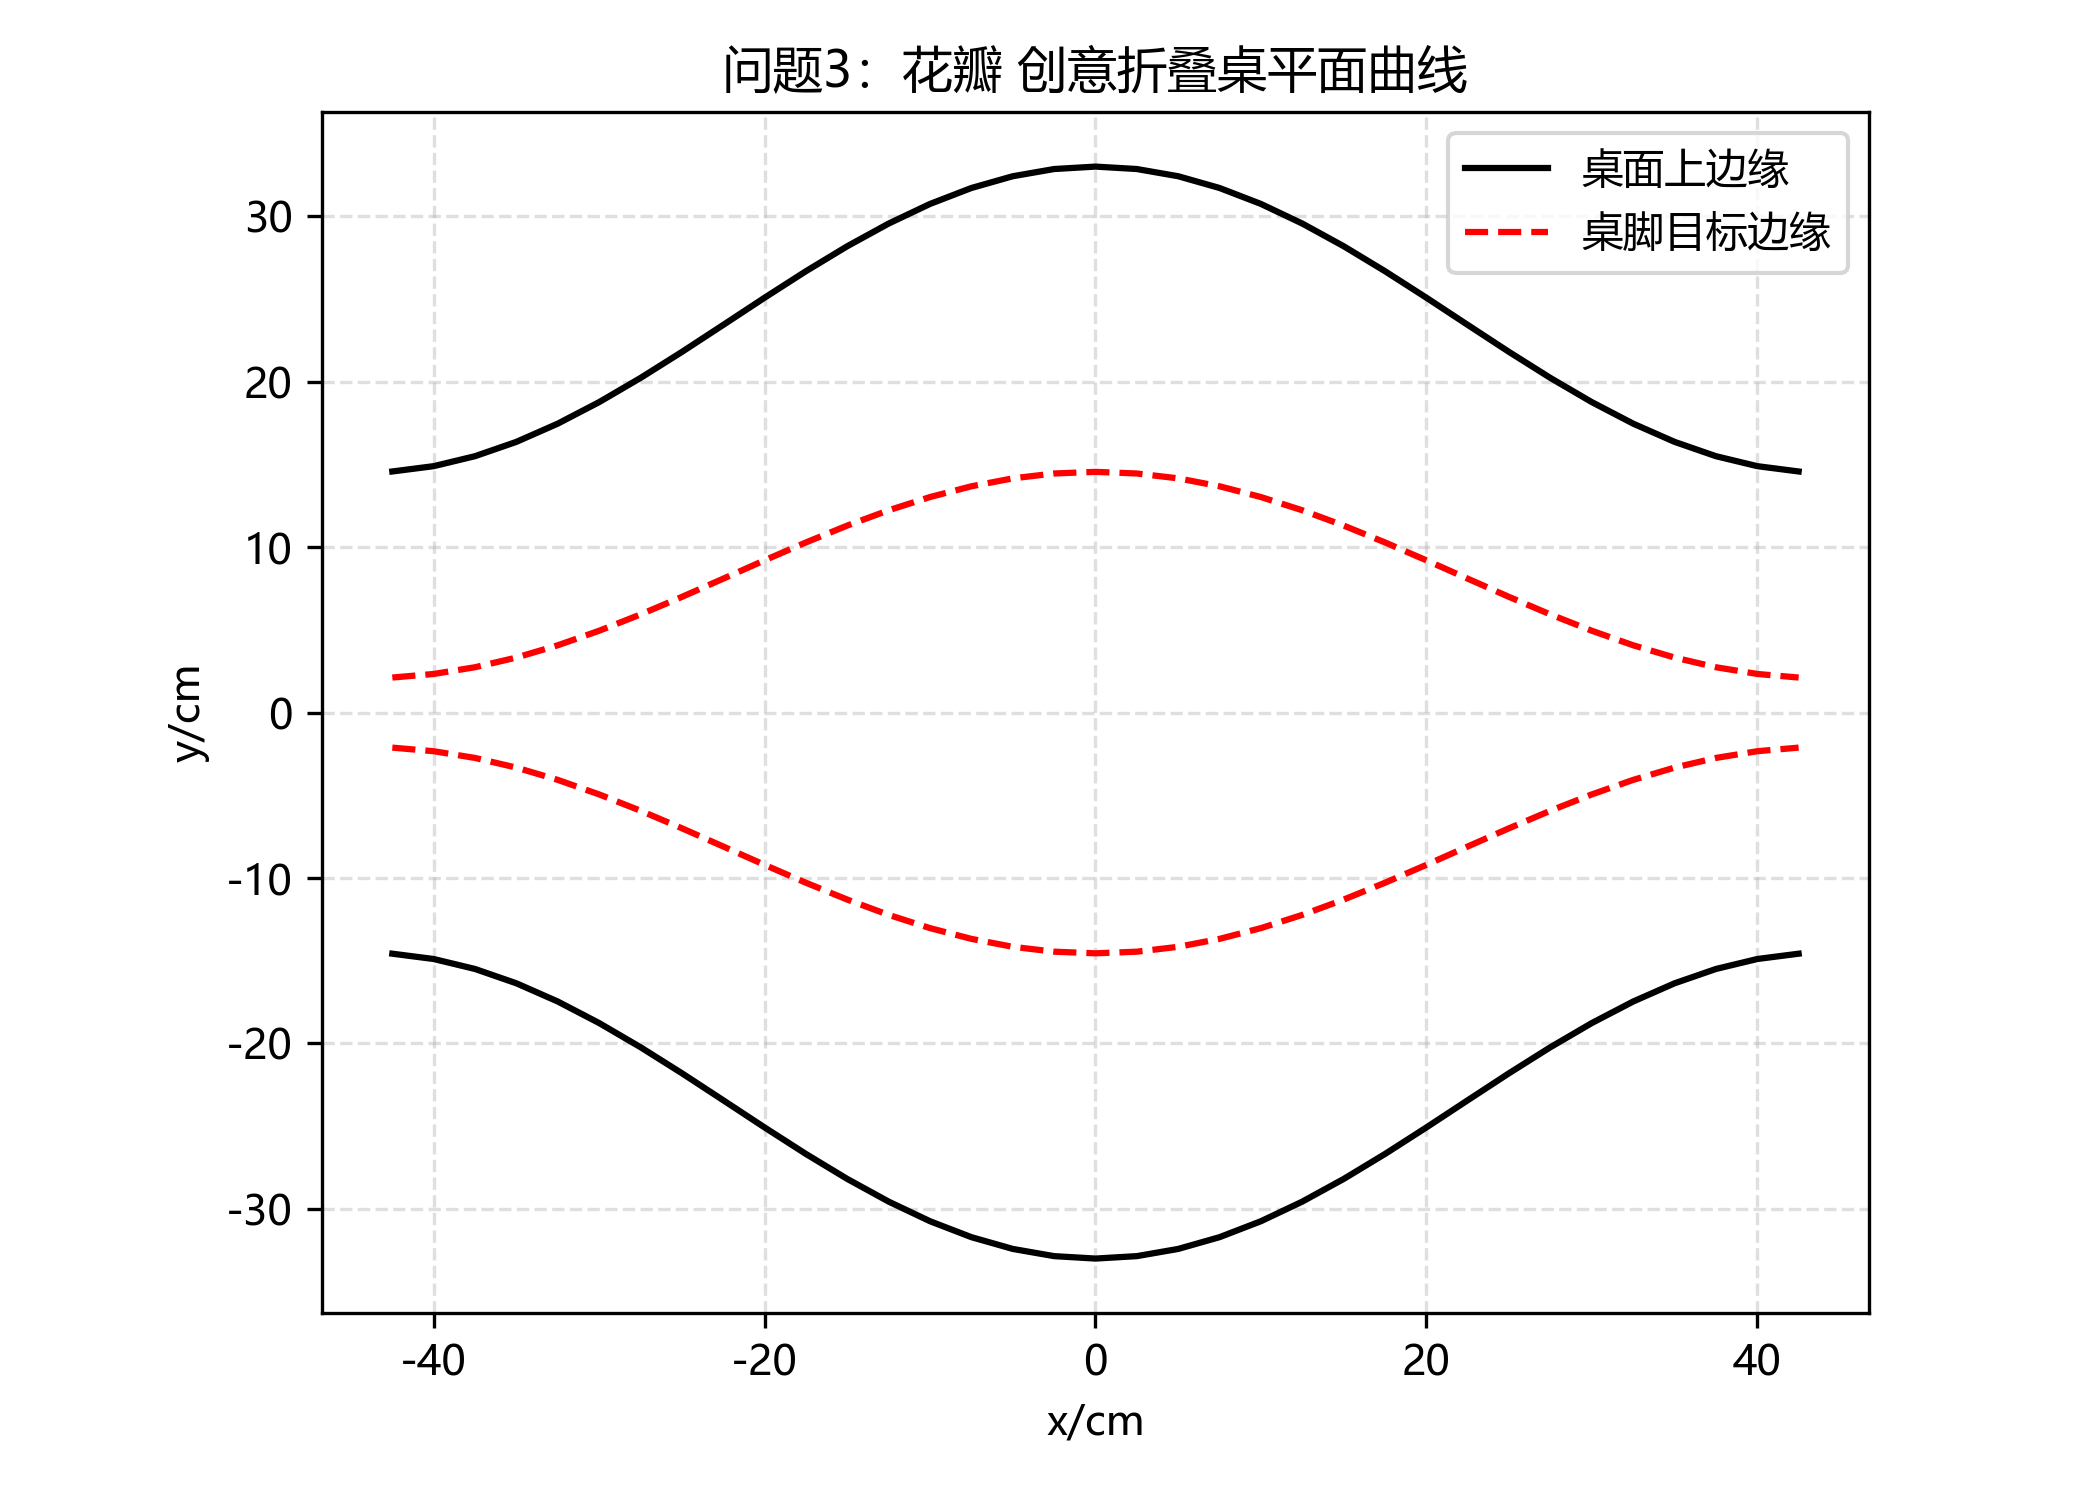
\includegraphics[width=\textwidth]{q3_petal_curves.png}\caption{花瓣}\end{subfigure}
\caption{三类创意折叠桌的桌面边界与桌脚边界}
\label{fig:q3curves}
\end{figure}
图\ref{fig:q3curves}展示了三类创意桌的平面曲线。黑线为桌面边界，红线为桌脚目标边界。可以看出，桌脚边界均被控制在桌面投影内部，避免了外扩造成的碰撞和不美观；同时不同形状保留了明显的外观差异，满足设计软件的个性化需求。

\begin{figure}[H]
\centering
\begin{subfigure}{0.32\textwidth}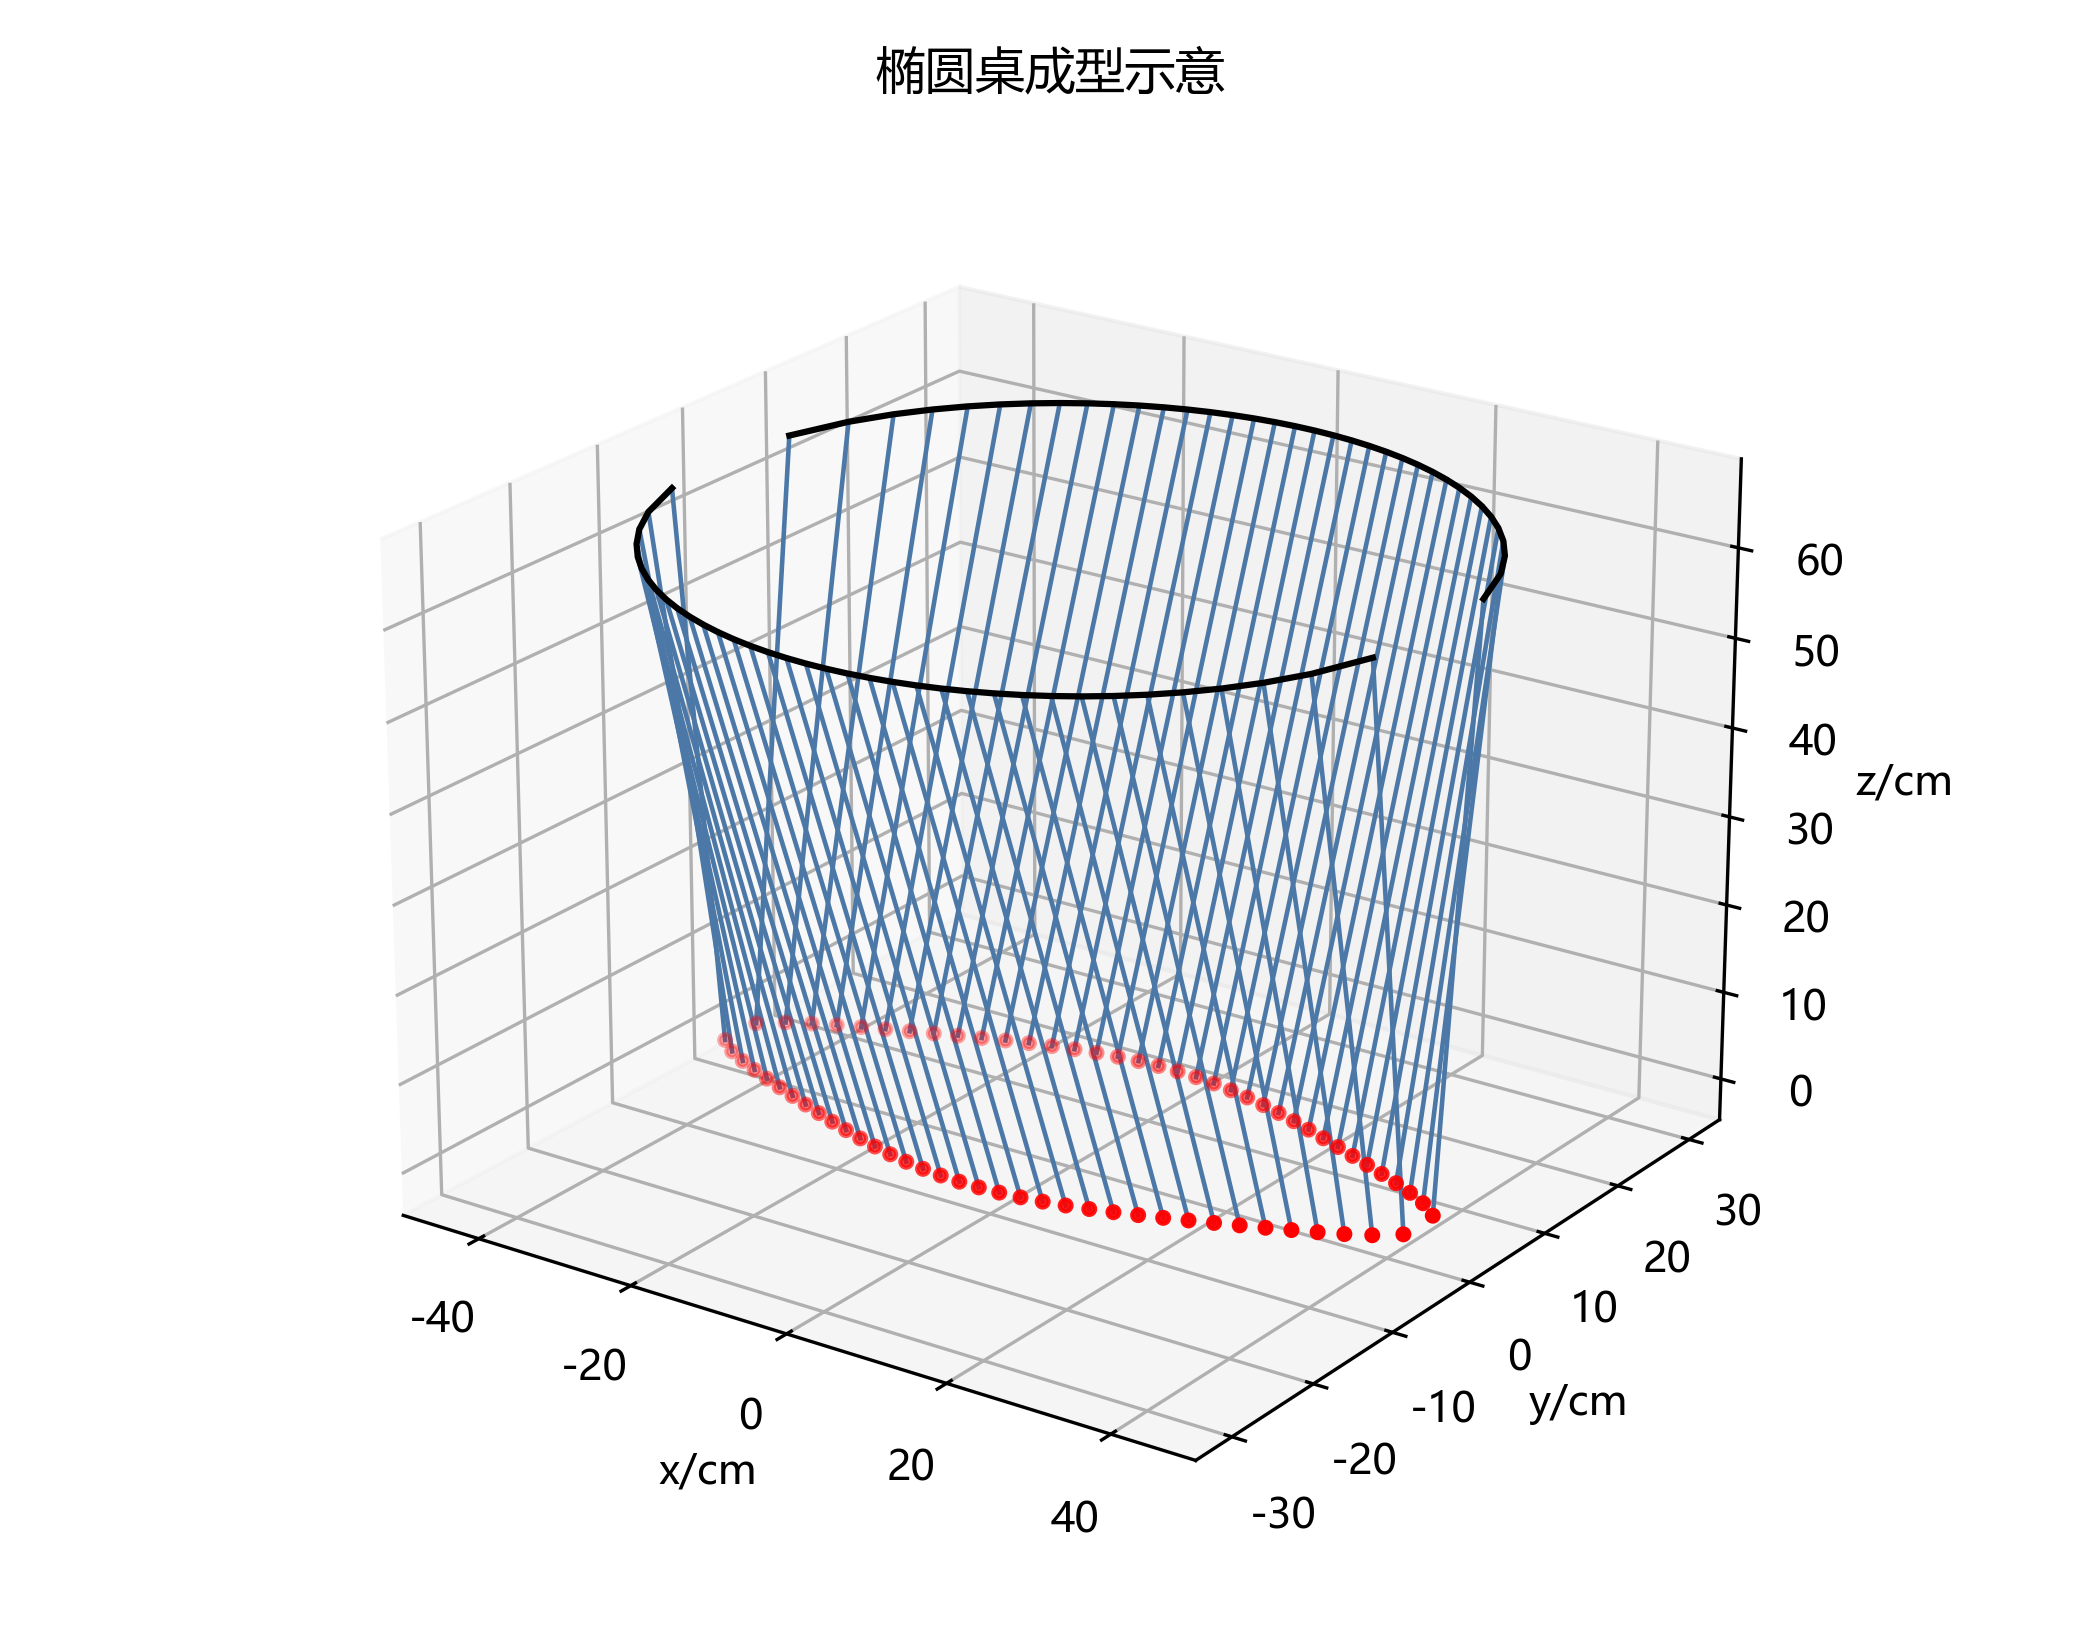
\includegraphics[width=\textwidth]{q3_ellipse_3d.png}\caption{椭圆成型}\end{subfigure}
\begin{subfigure}{0.32\textwidth}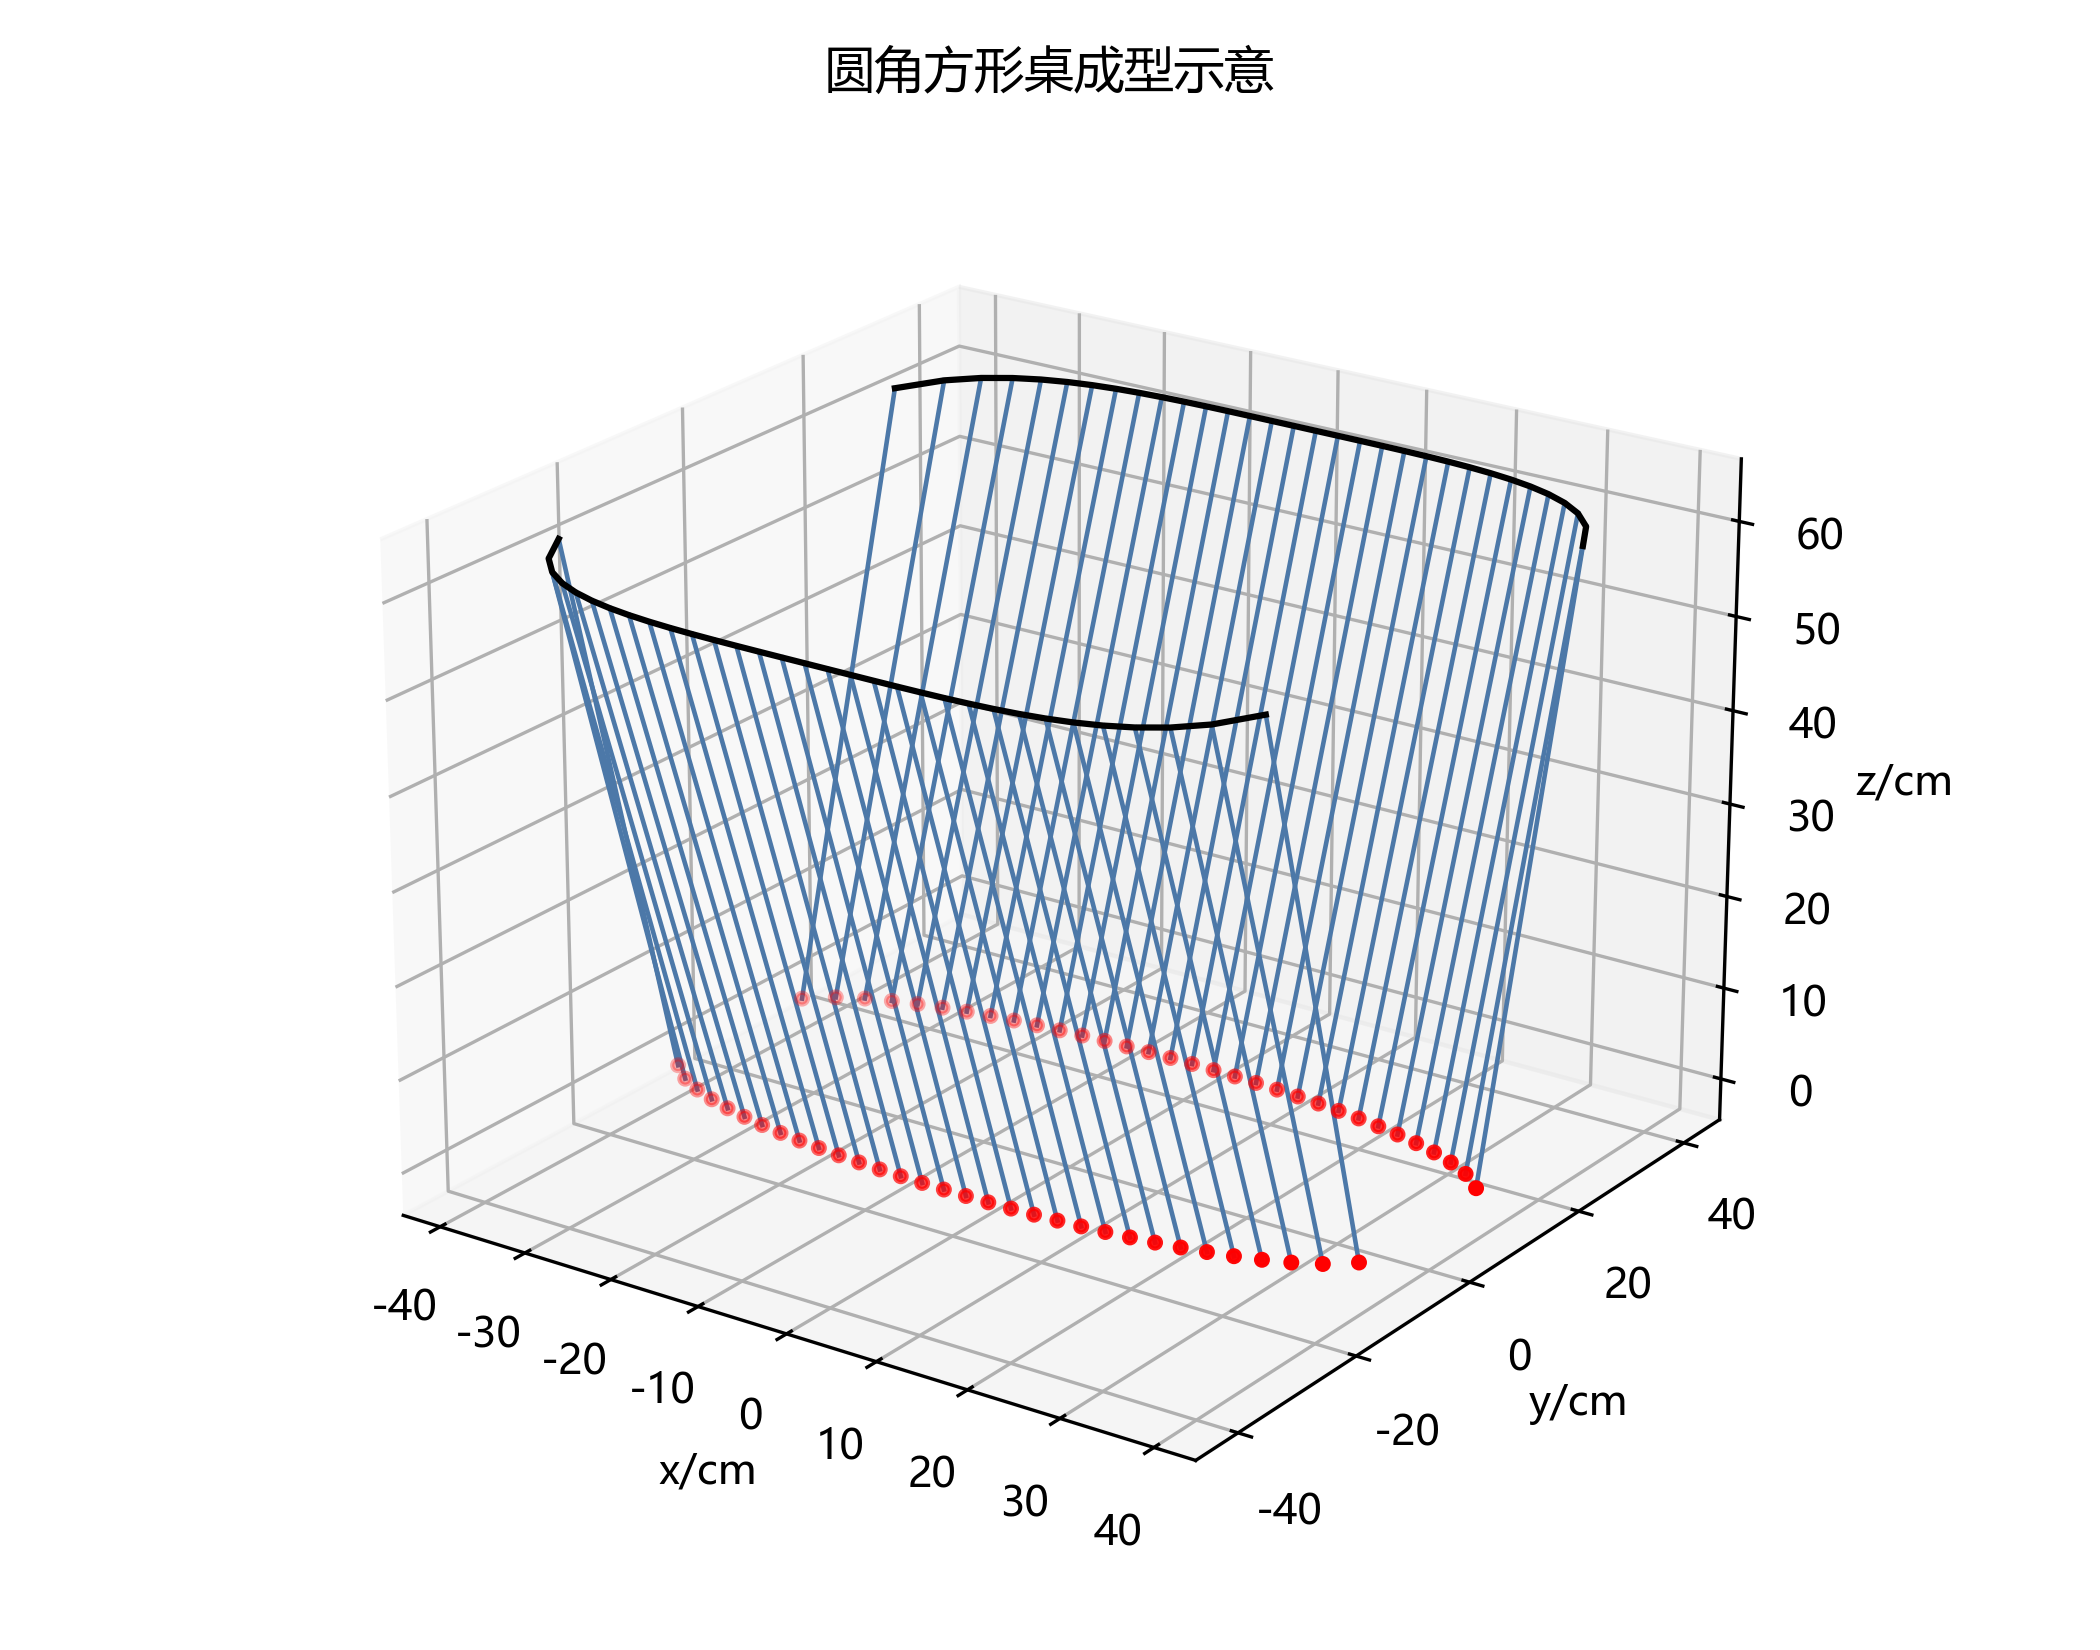
\includegraphics[width=\textwidth]{q3_rounded_square_3d.png}\caption{圆角方形成型}\end{subfigure}
\begin{subfigure}{0.32\textwidth}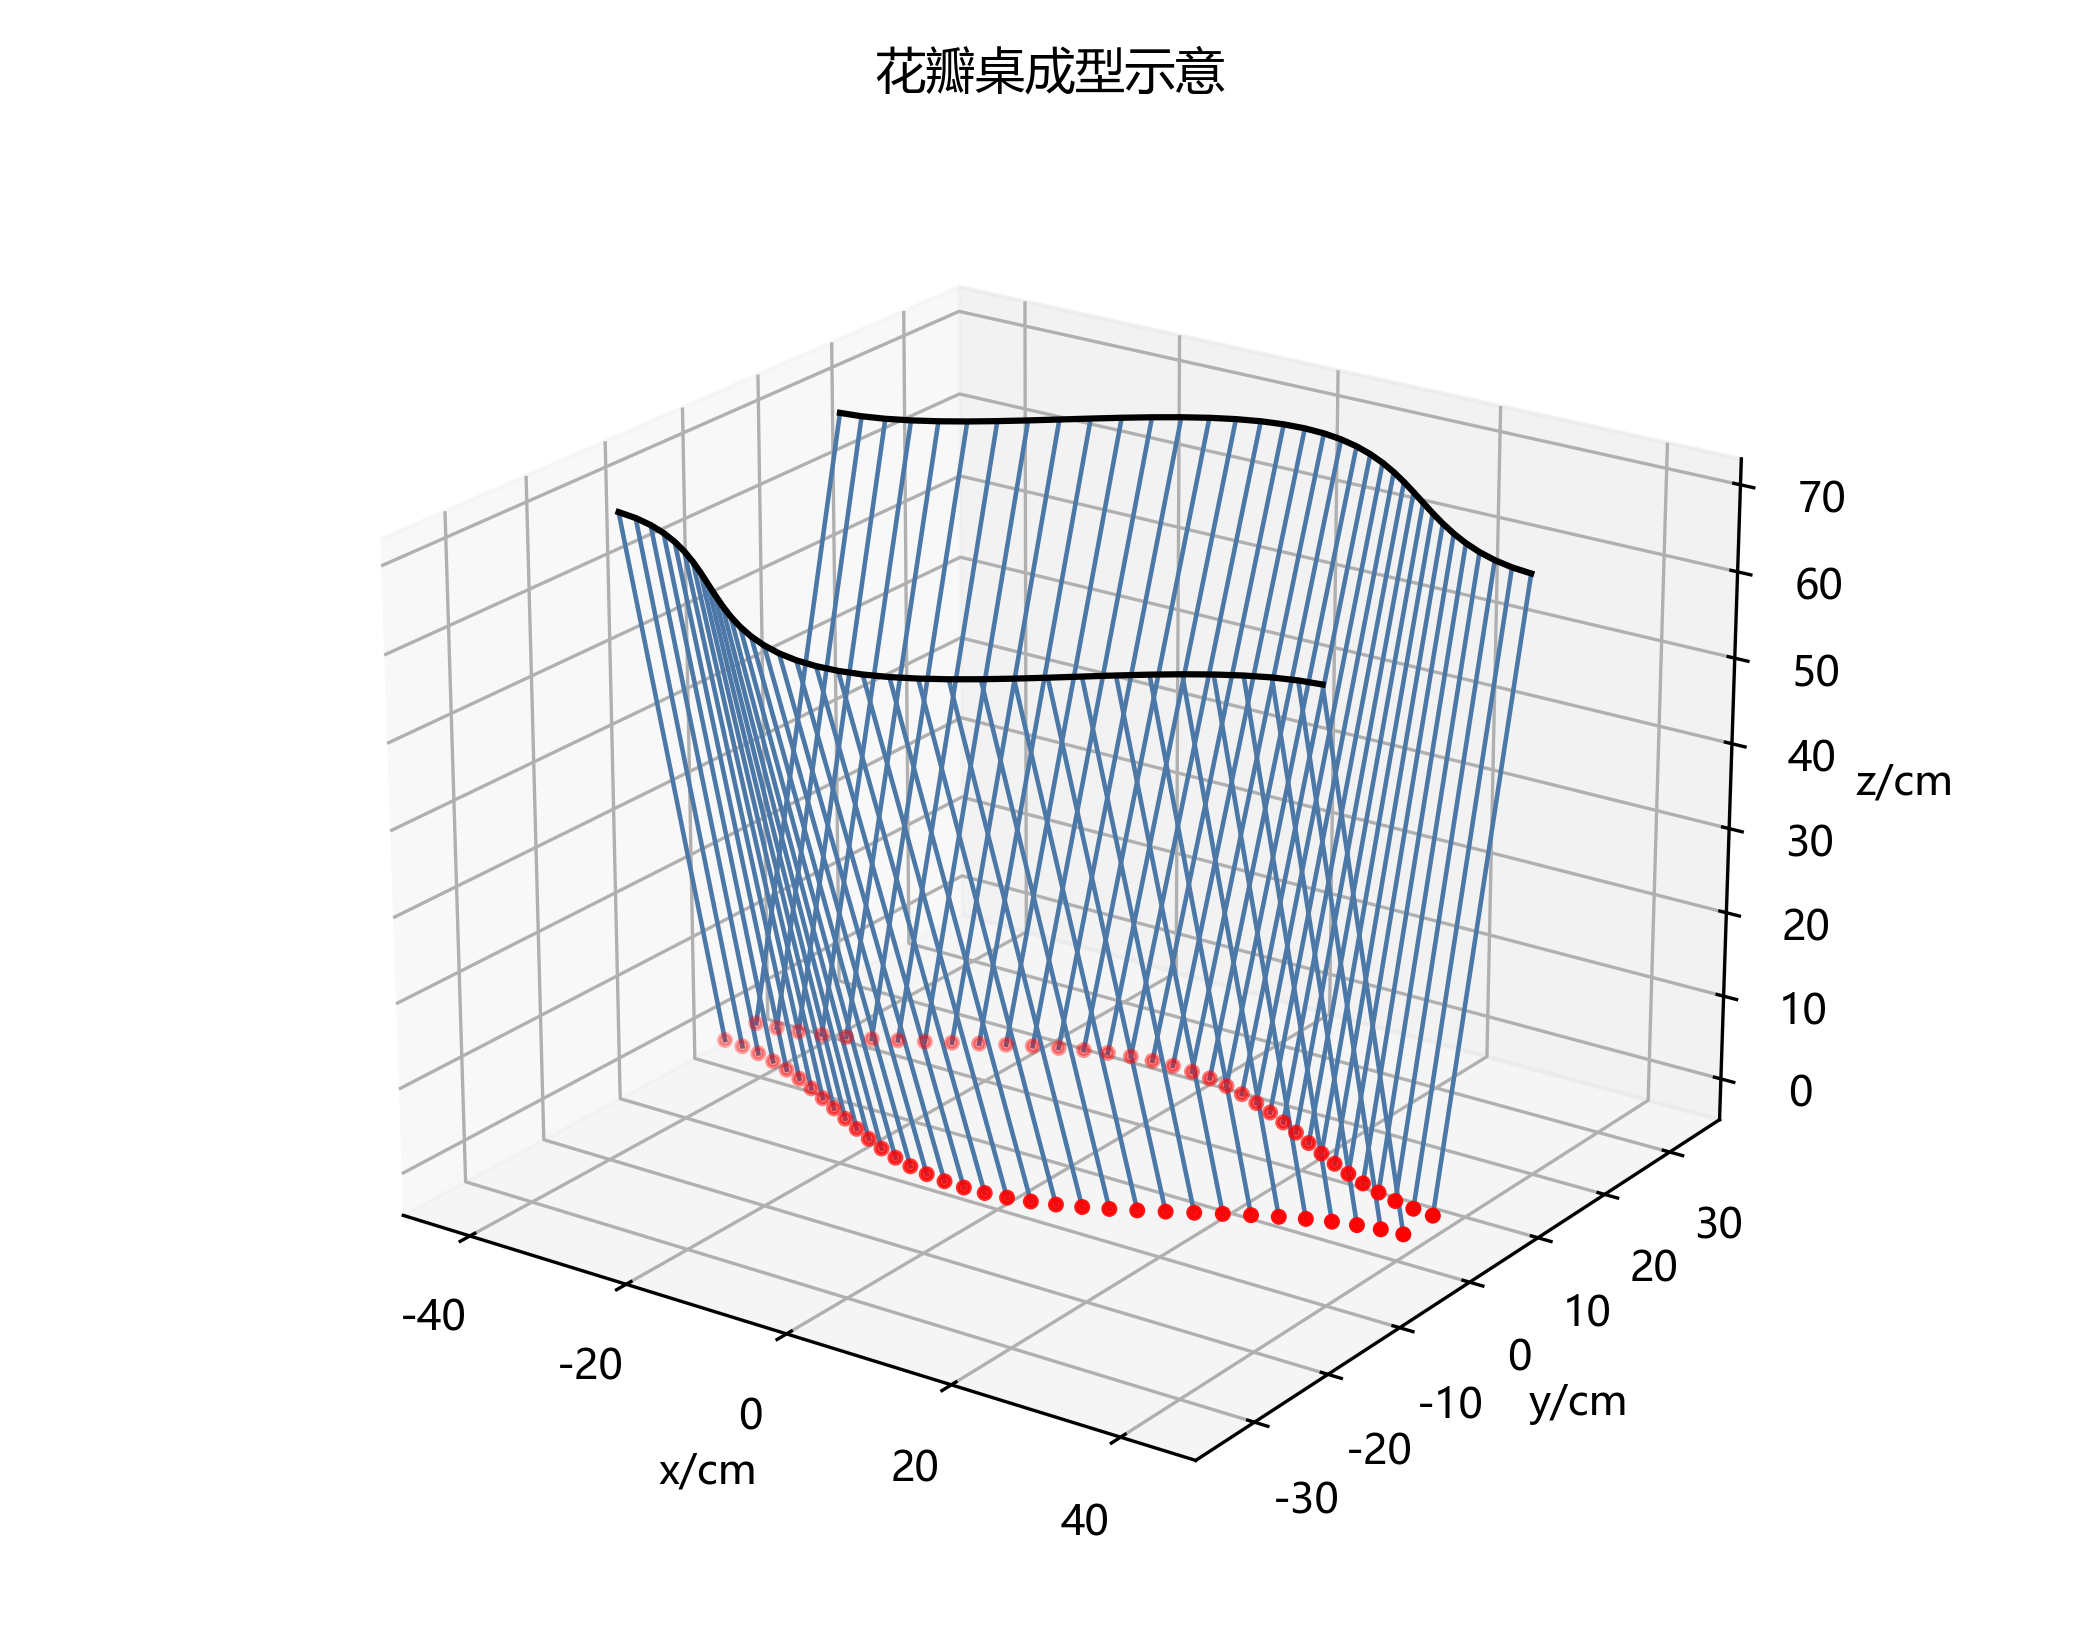
\includegraphics[width=\textwidth]{q3_petal_3d.png}\caption{花瓣成型}\end{subfigure}
\caption{三类创意折叠桌成型示意图}
\label{fig:q33d}
\end{figure}
图\ref{fig:q33d}表明，三类设计都能形成由木条母线构成的空间支撑面。虽然本文未进行结构有限元分析，但从几何角度看，各木条长度变化连续、桌脚边界闭合且支撑范围充分，满足概念设计阶段的可制造性要求。

\begin{figure}[H]
\centering
\begin{subfigure}{0.24\textwidth}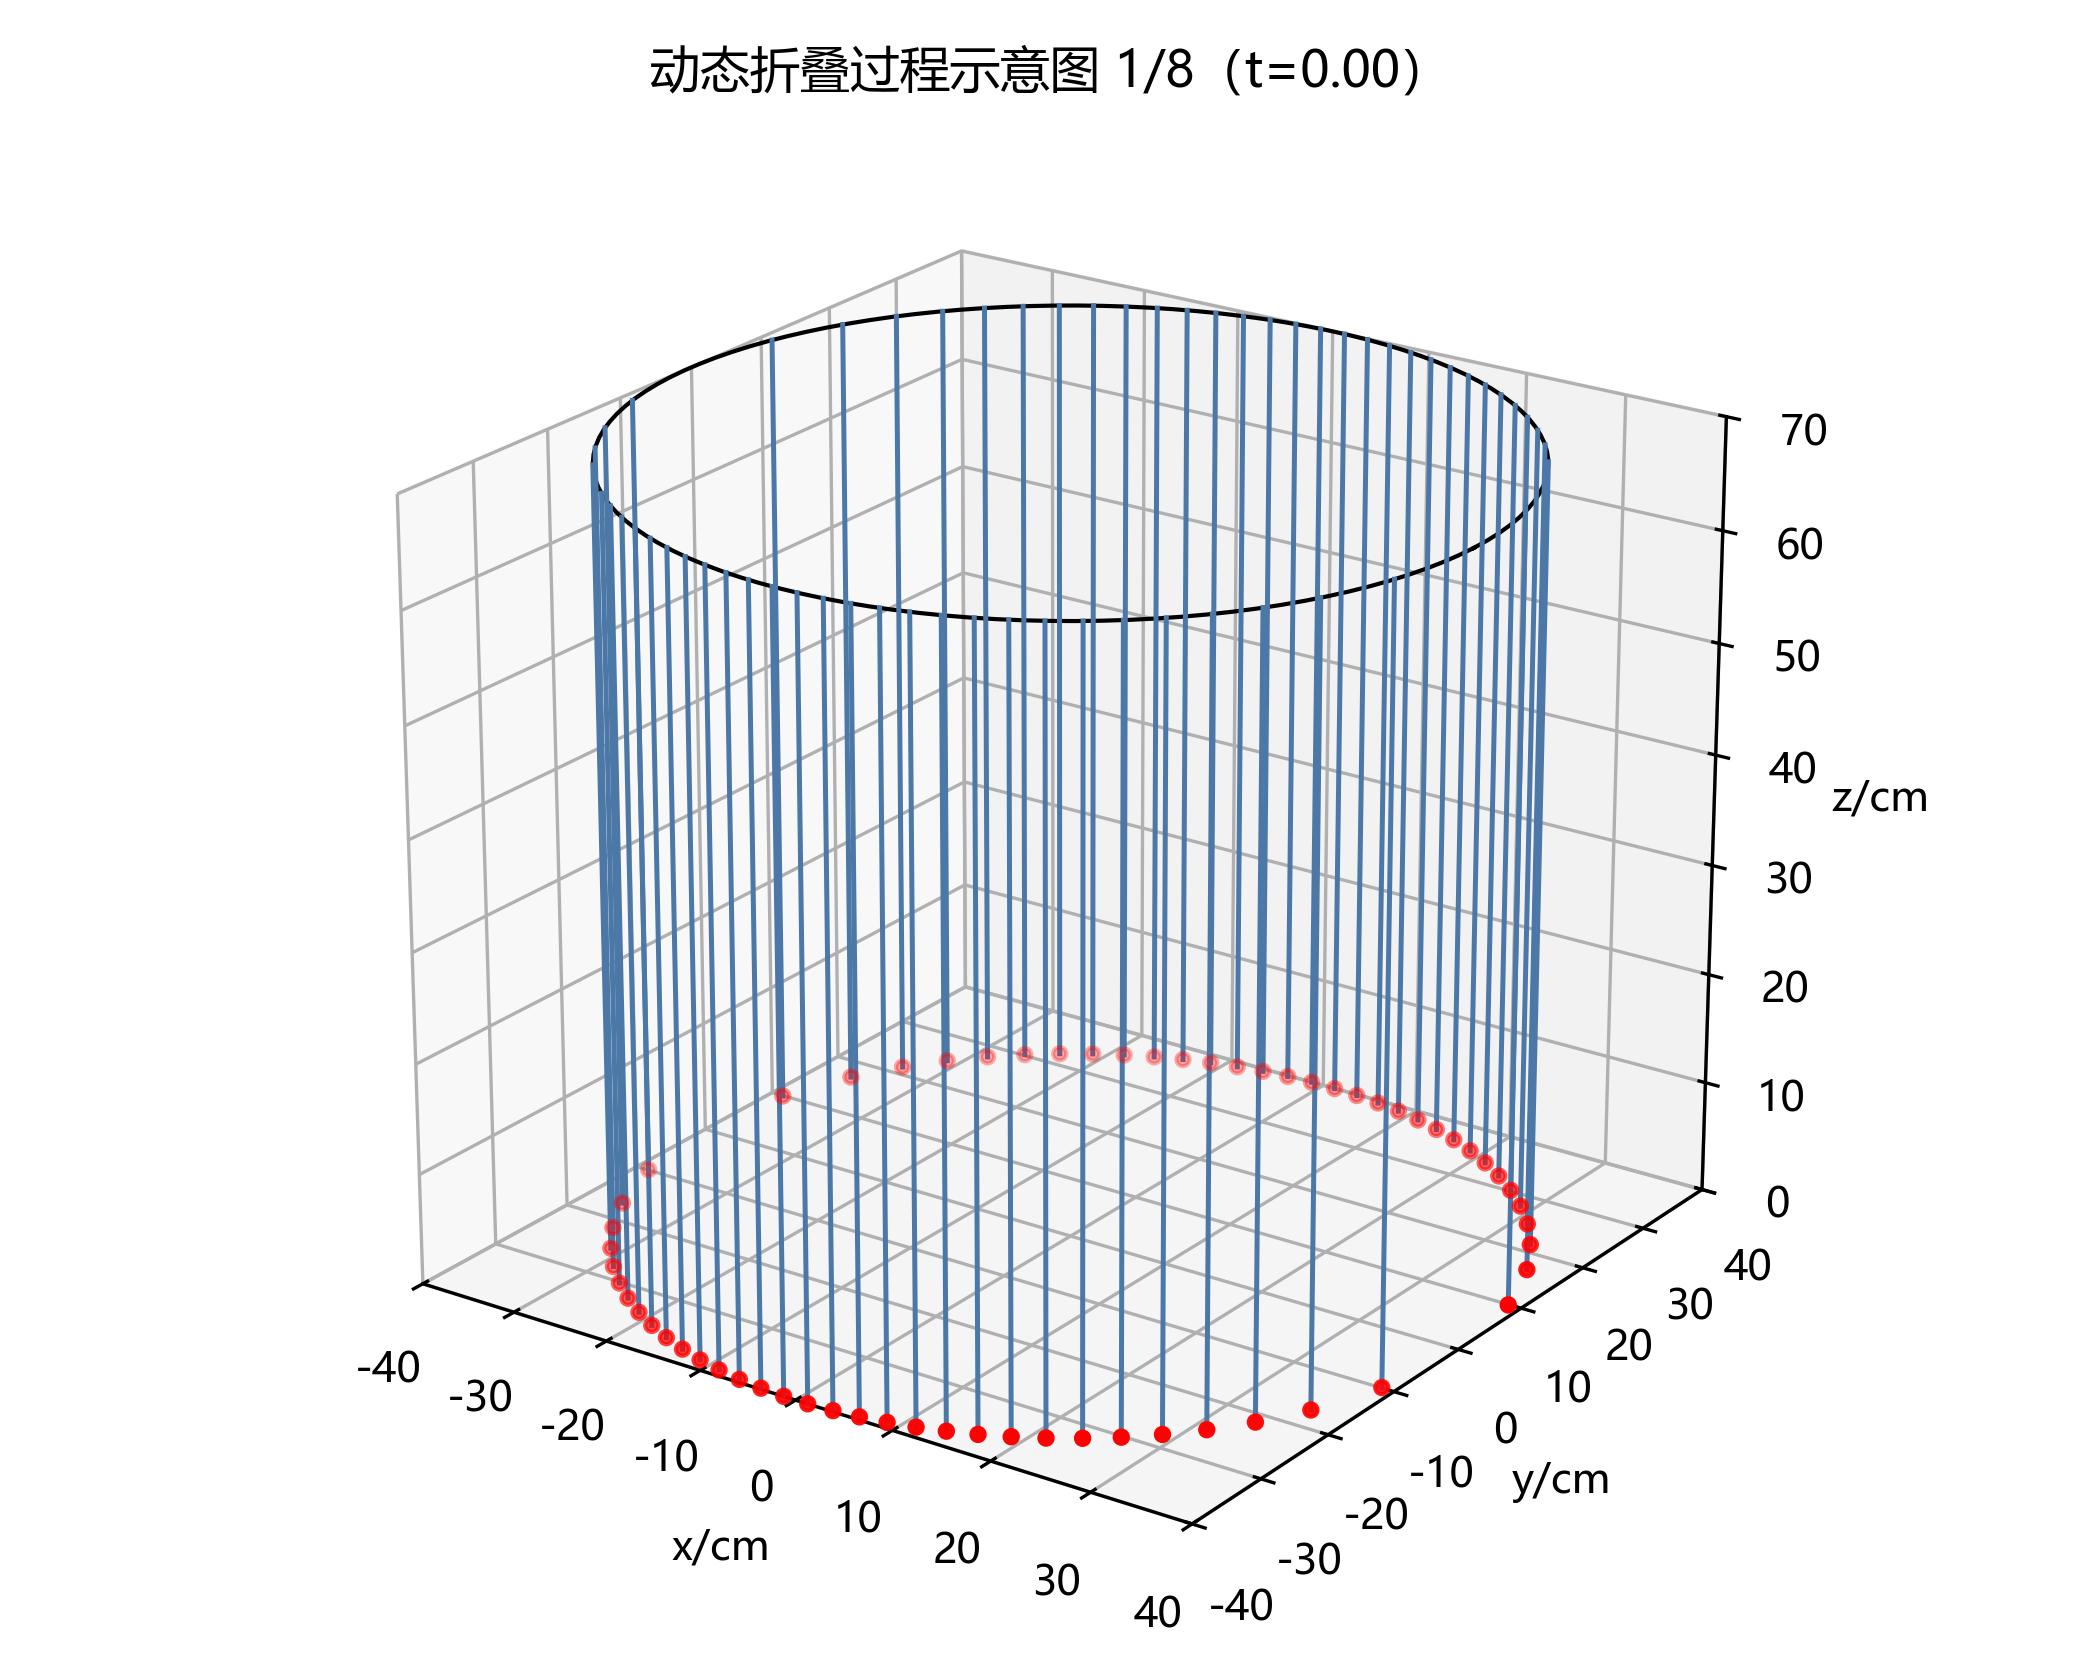
\includegraphics[width=\textwidth]{q3_software_dynamic_01.png}\caption{1}\end{subfigure}
\begin{subfigure}{0.24\textwidth}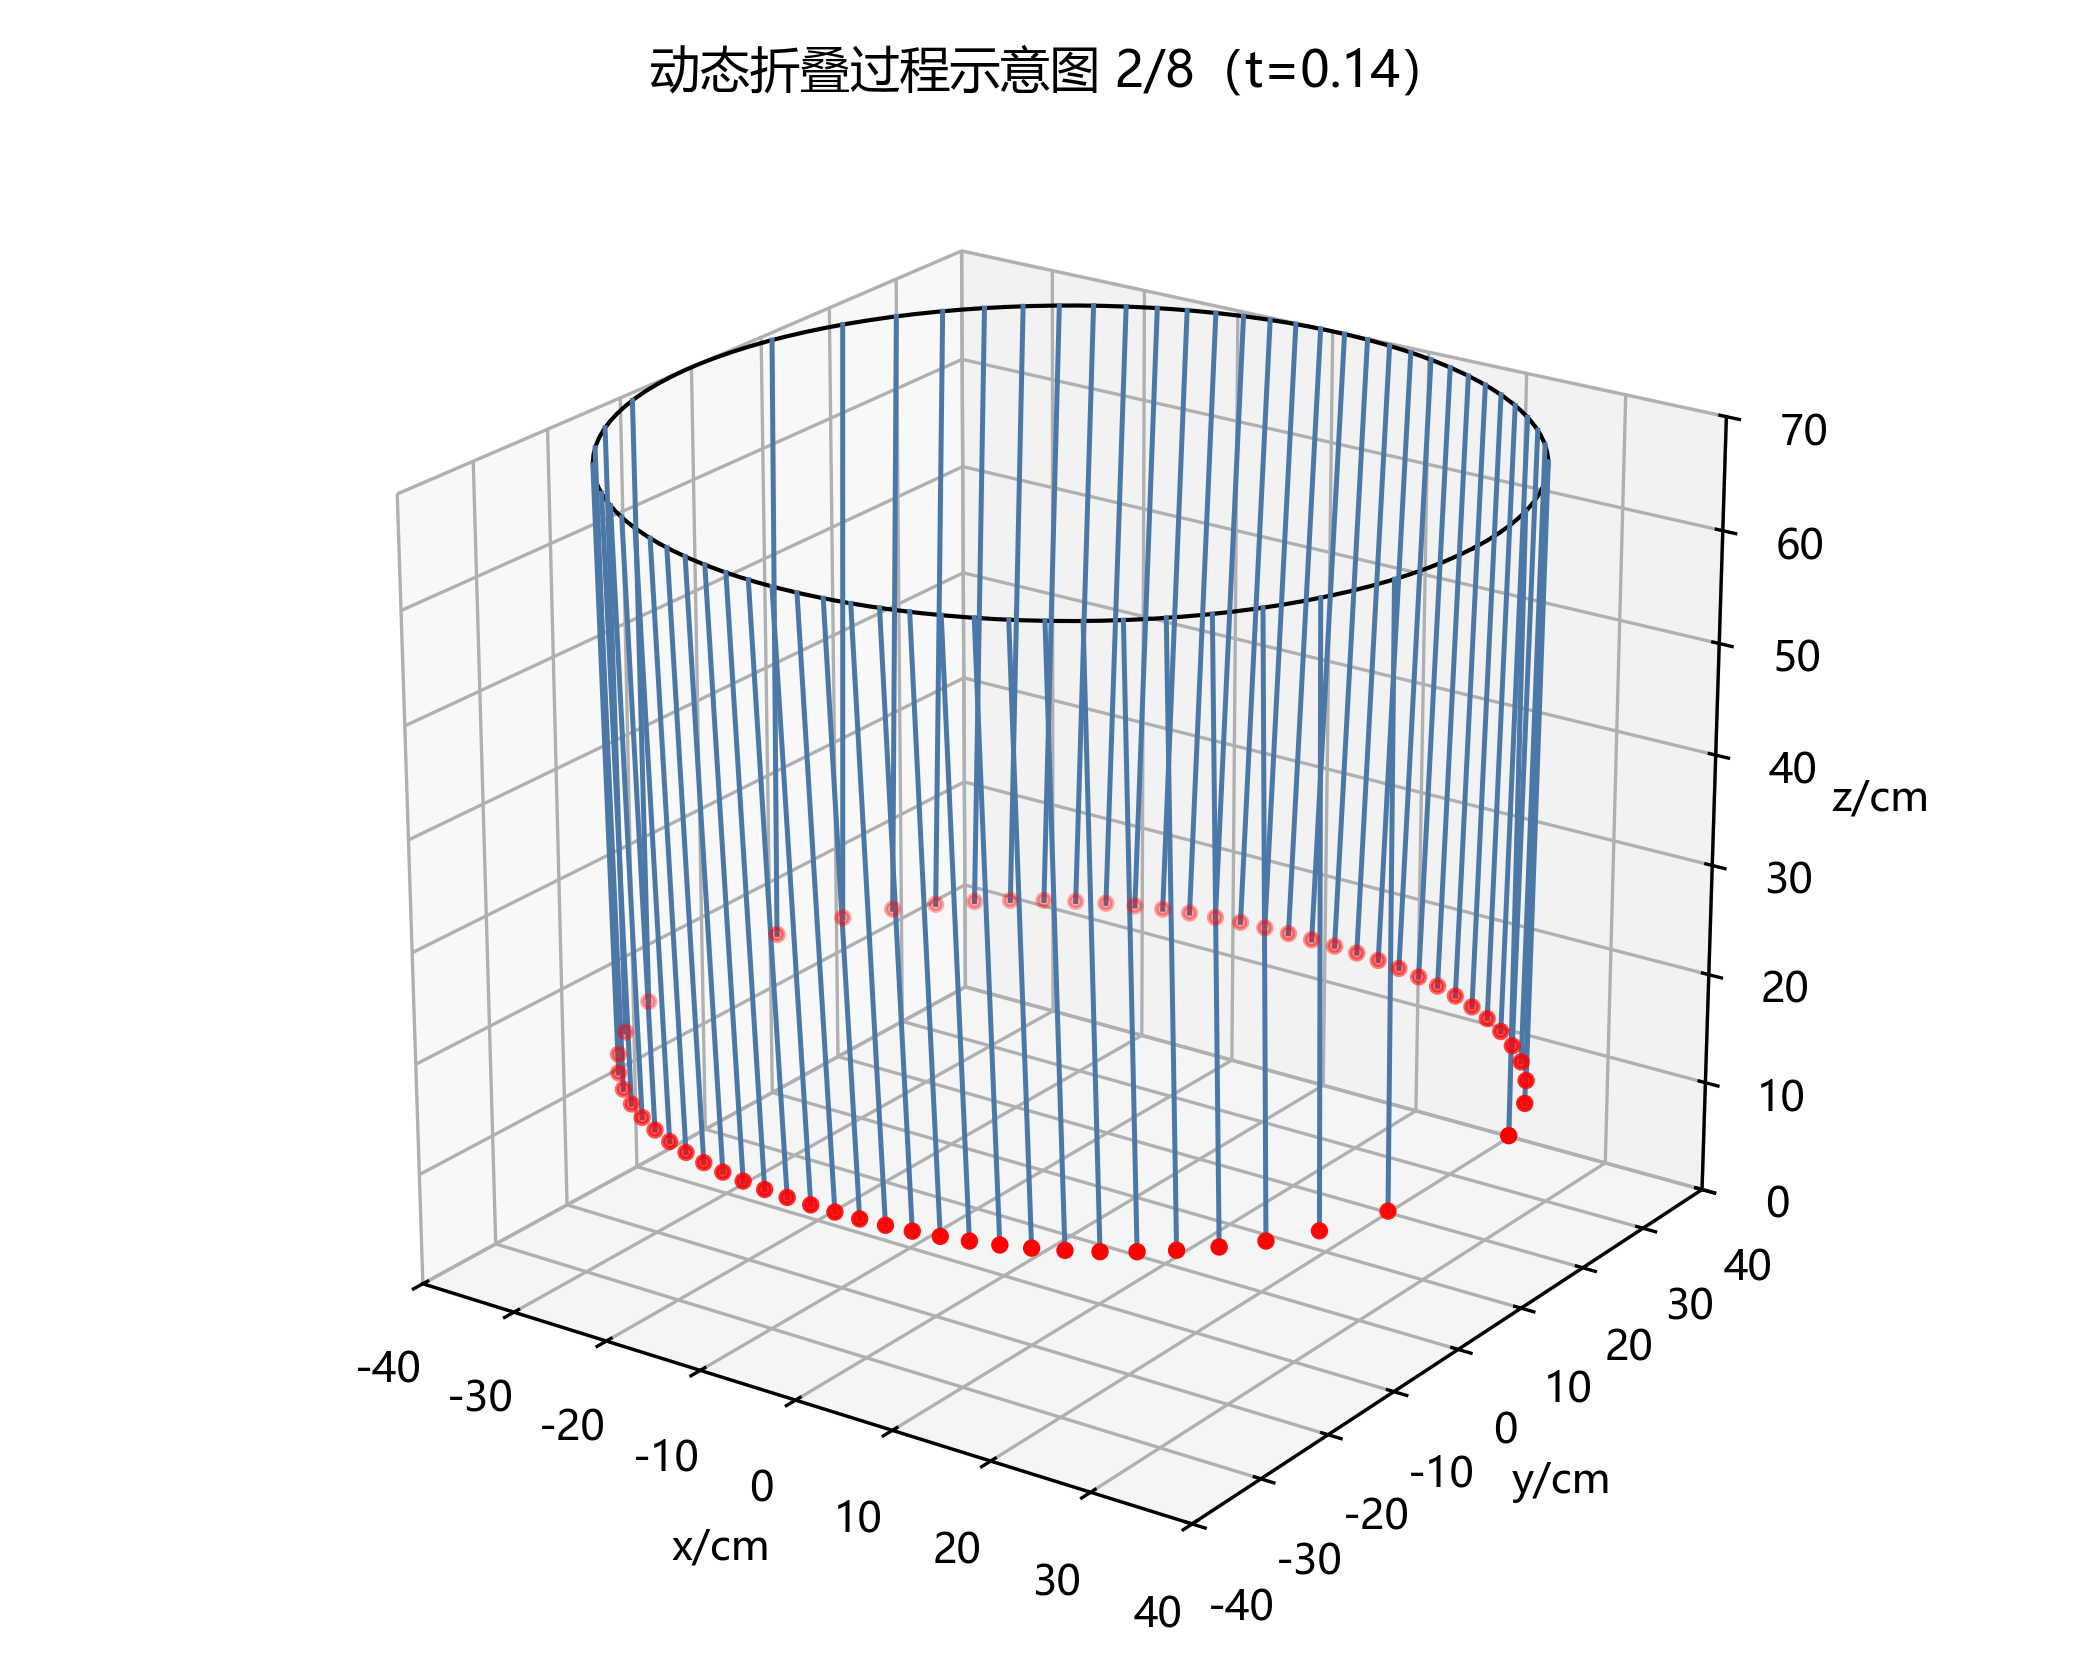
\includegraphics[width=\textwidth]{q3_software_dynamic_02.png}\caption{2}\end{subfigure}
\begin{subfigure}{0.24\textwidth}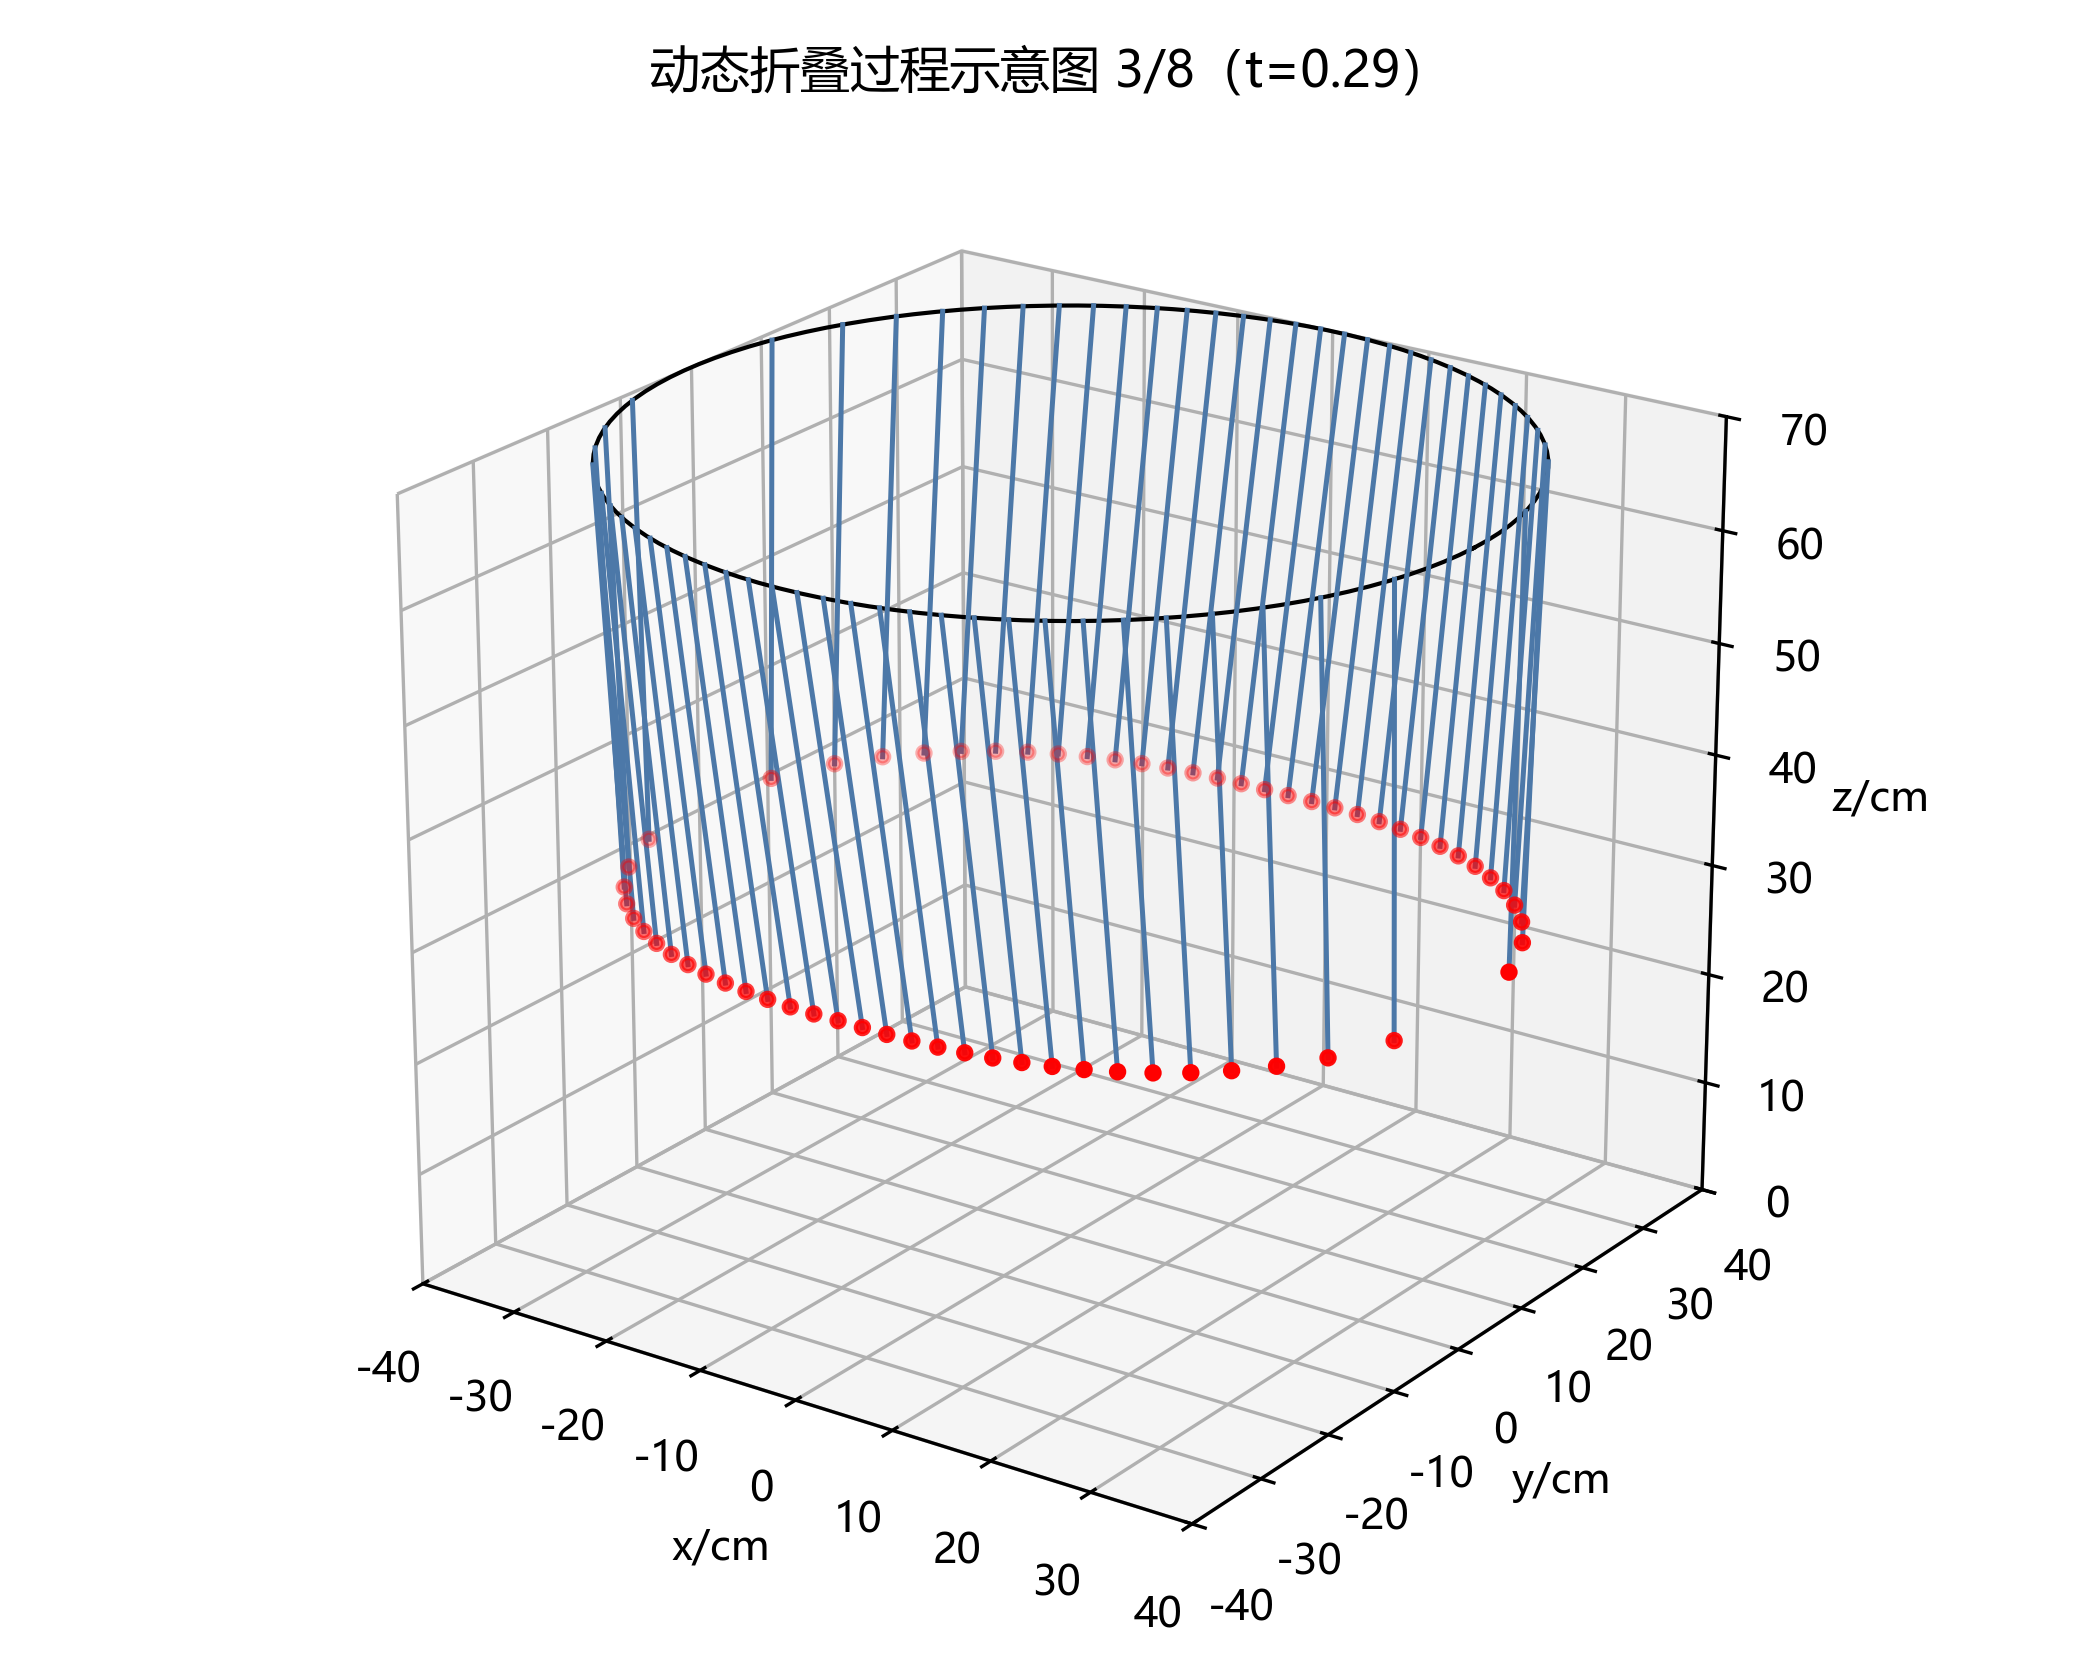
\includegraphics[width=\textwidth]{q3_software_dynamic_03.png}\caption{3}\end{subfigure}
\begin{subfigure}{0.24\textwidth}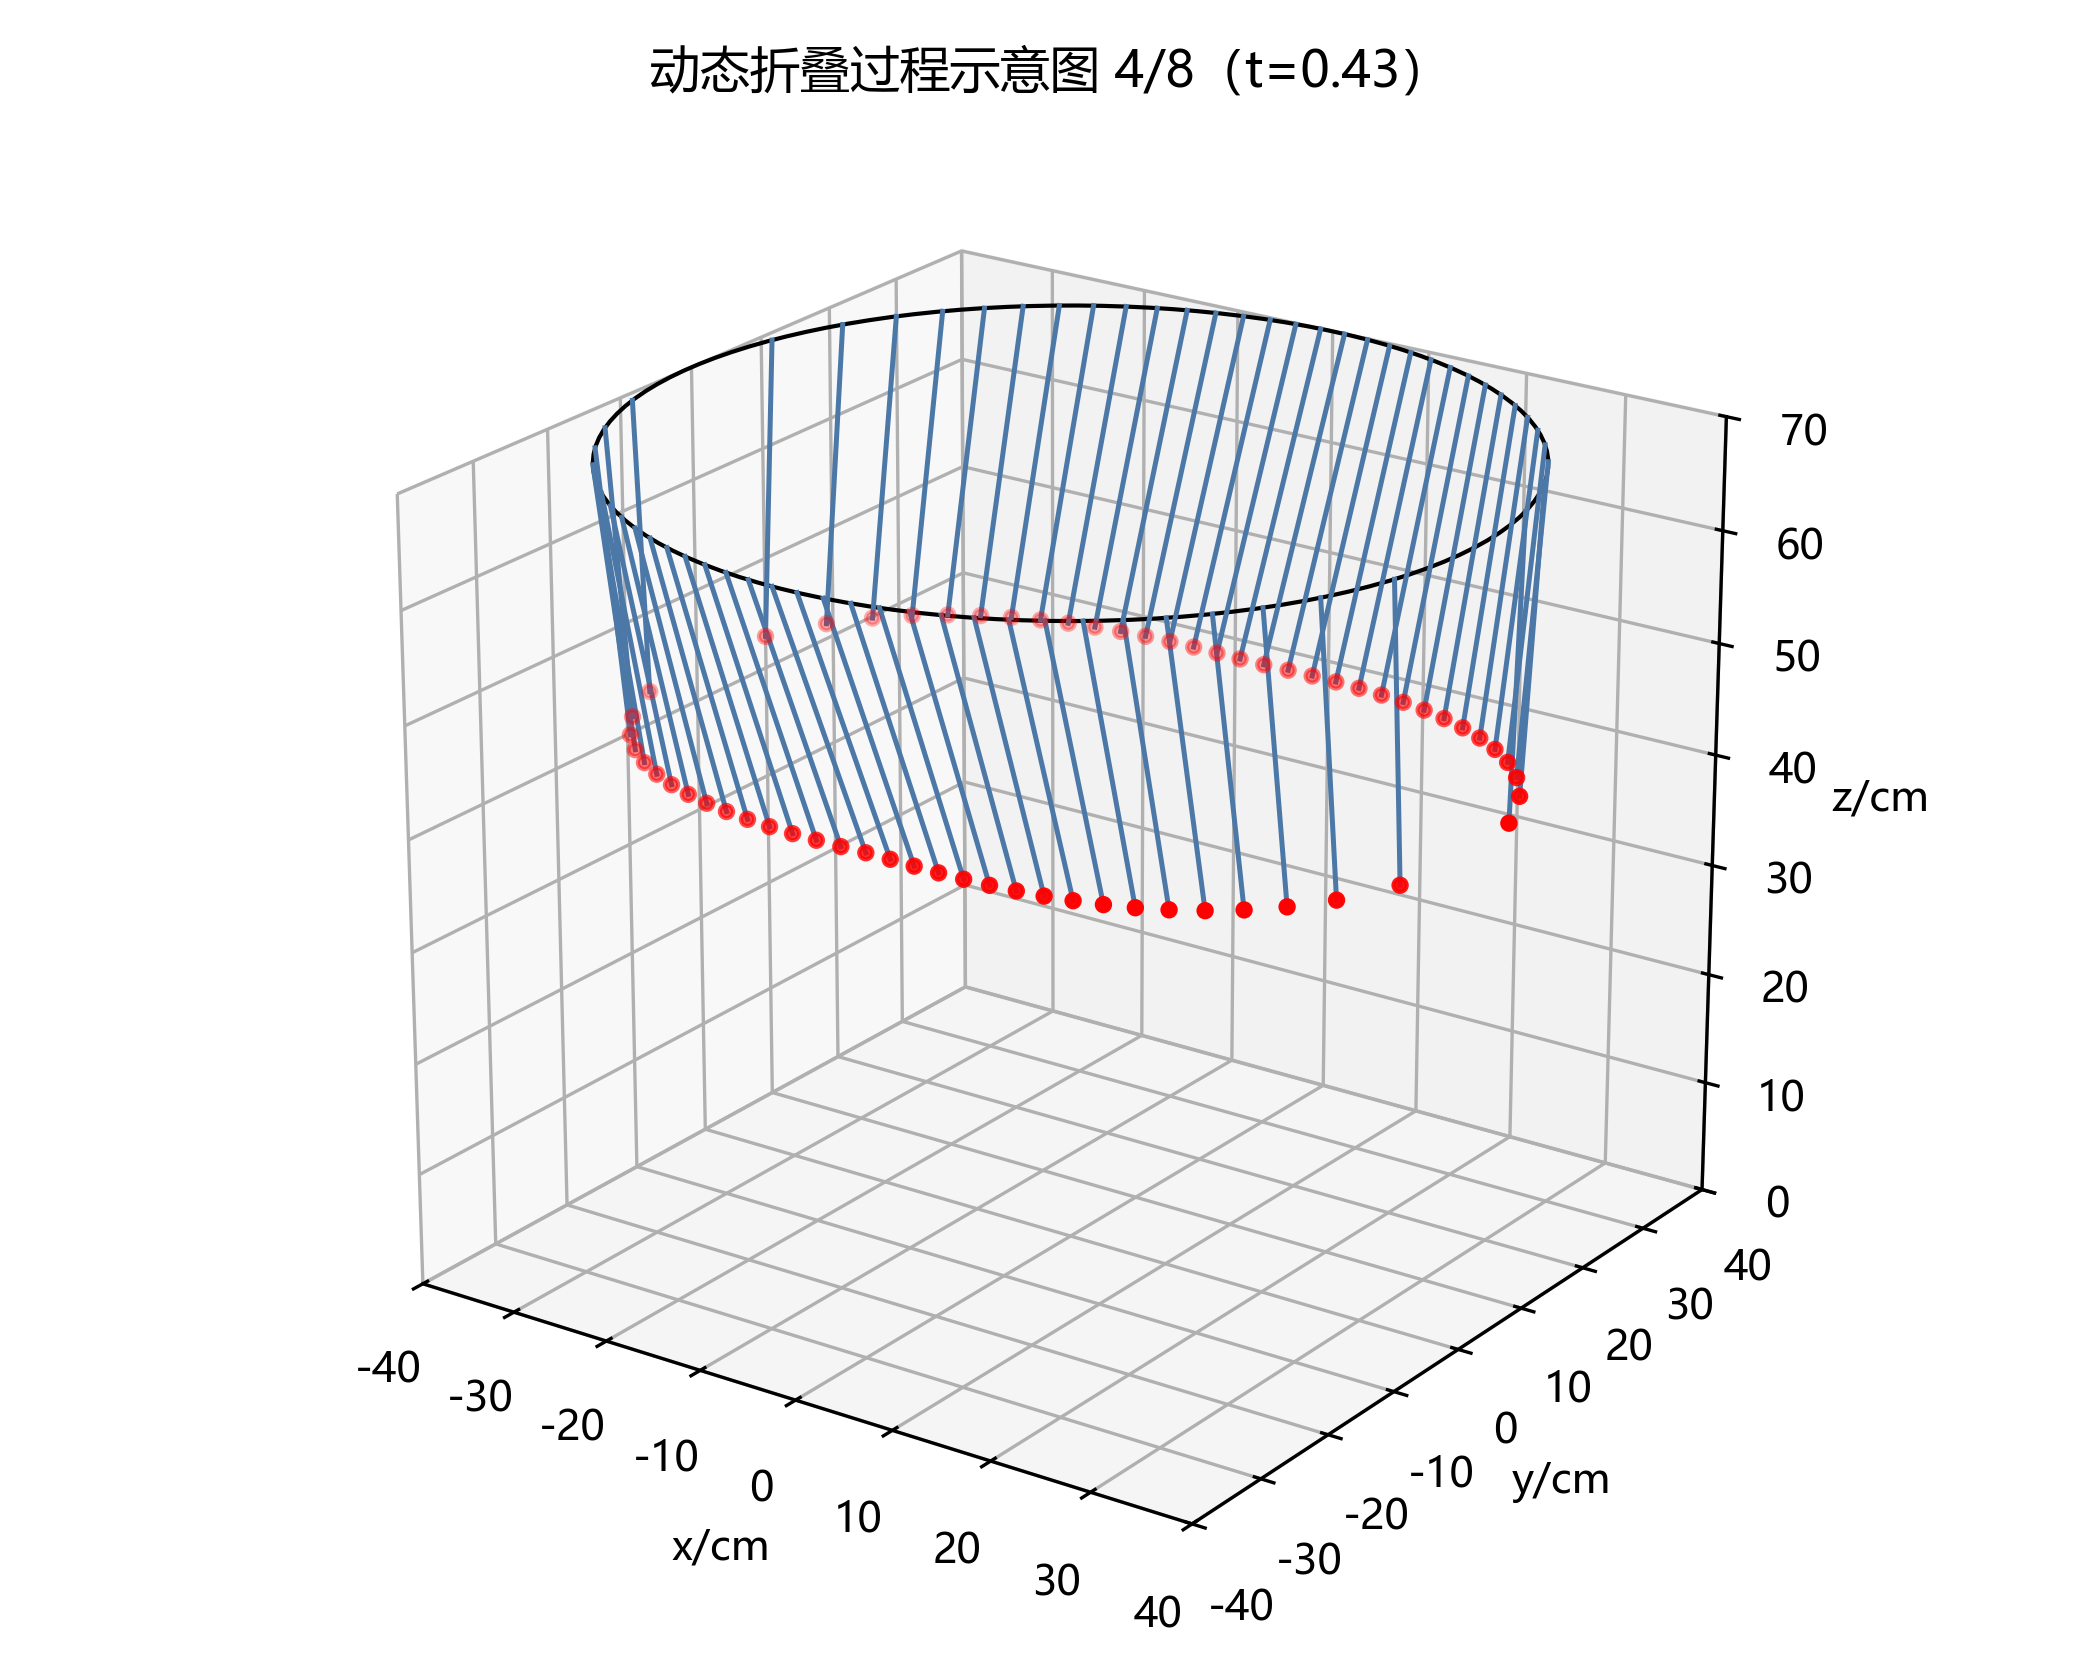
\includegraphics[width=\textwidth]{q3_software_dynamic_04.png}\caption{4}\end{subfigure}

\begin{subfigure}{0.24\textwidth}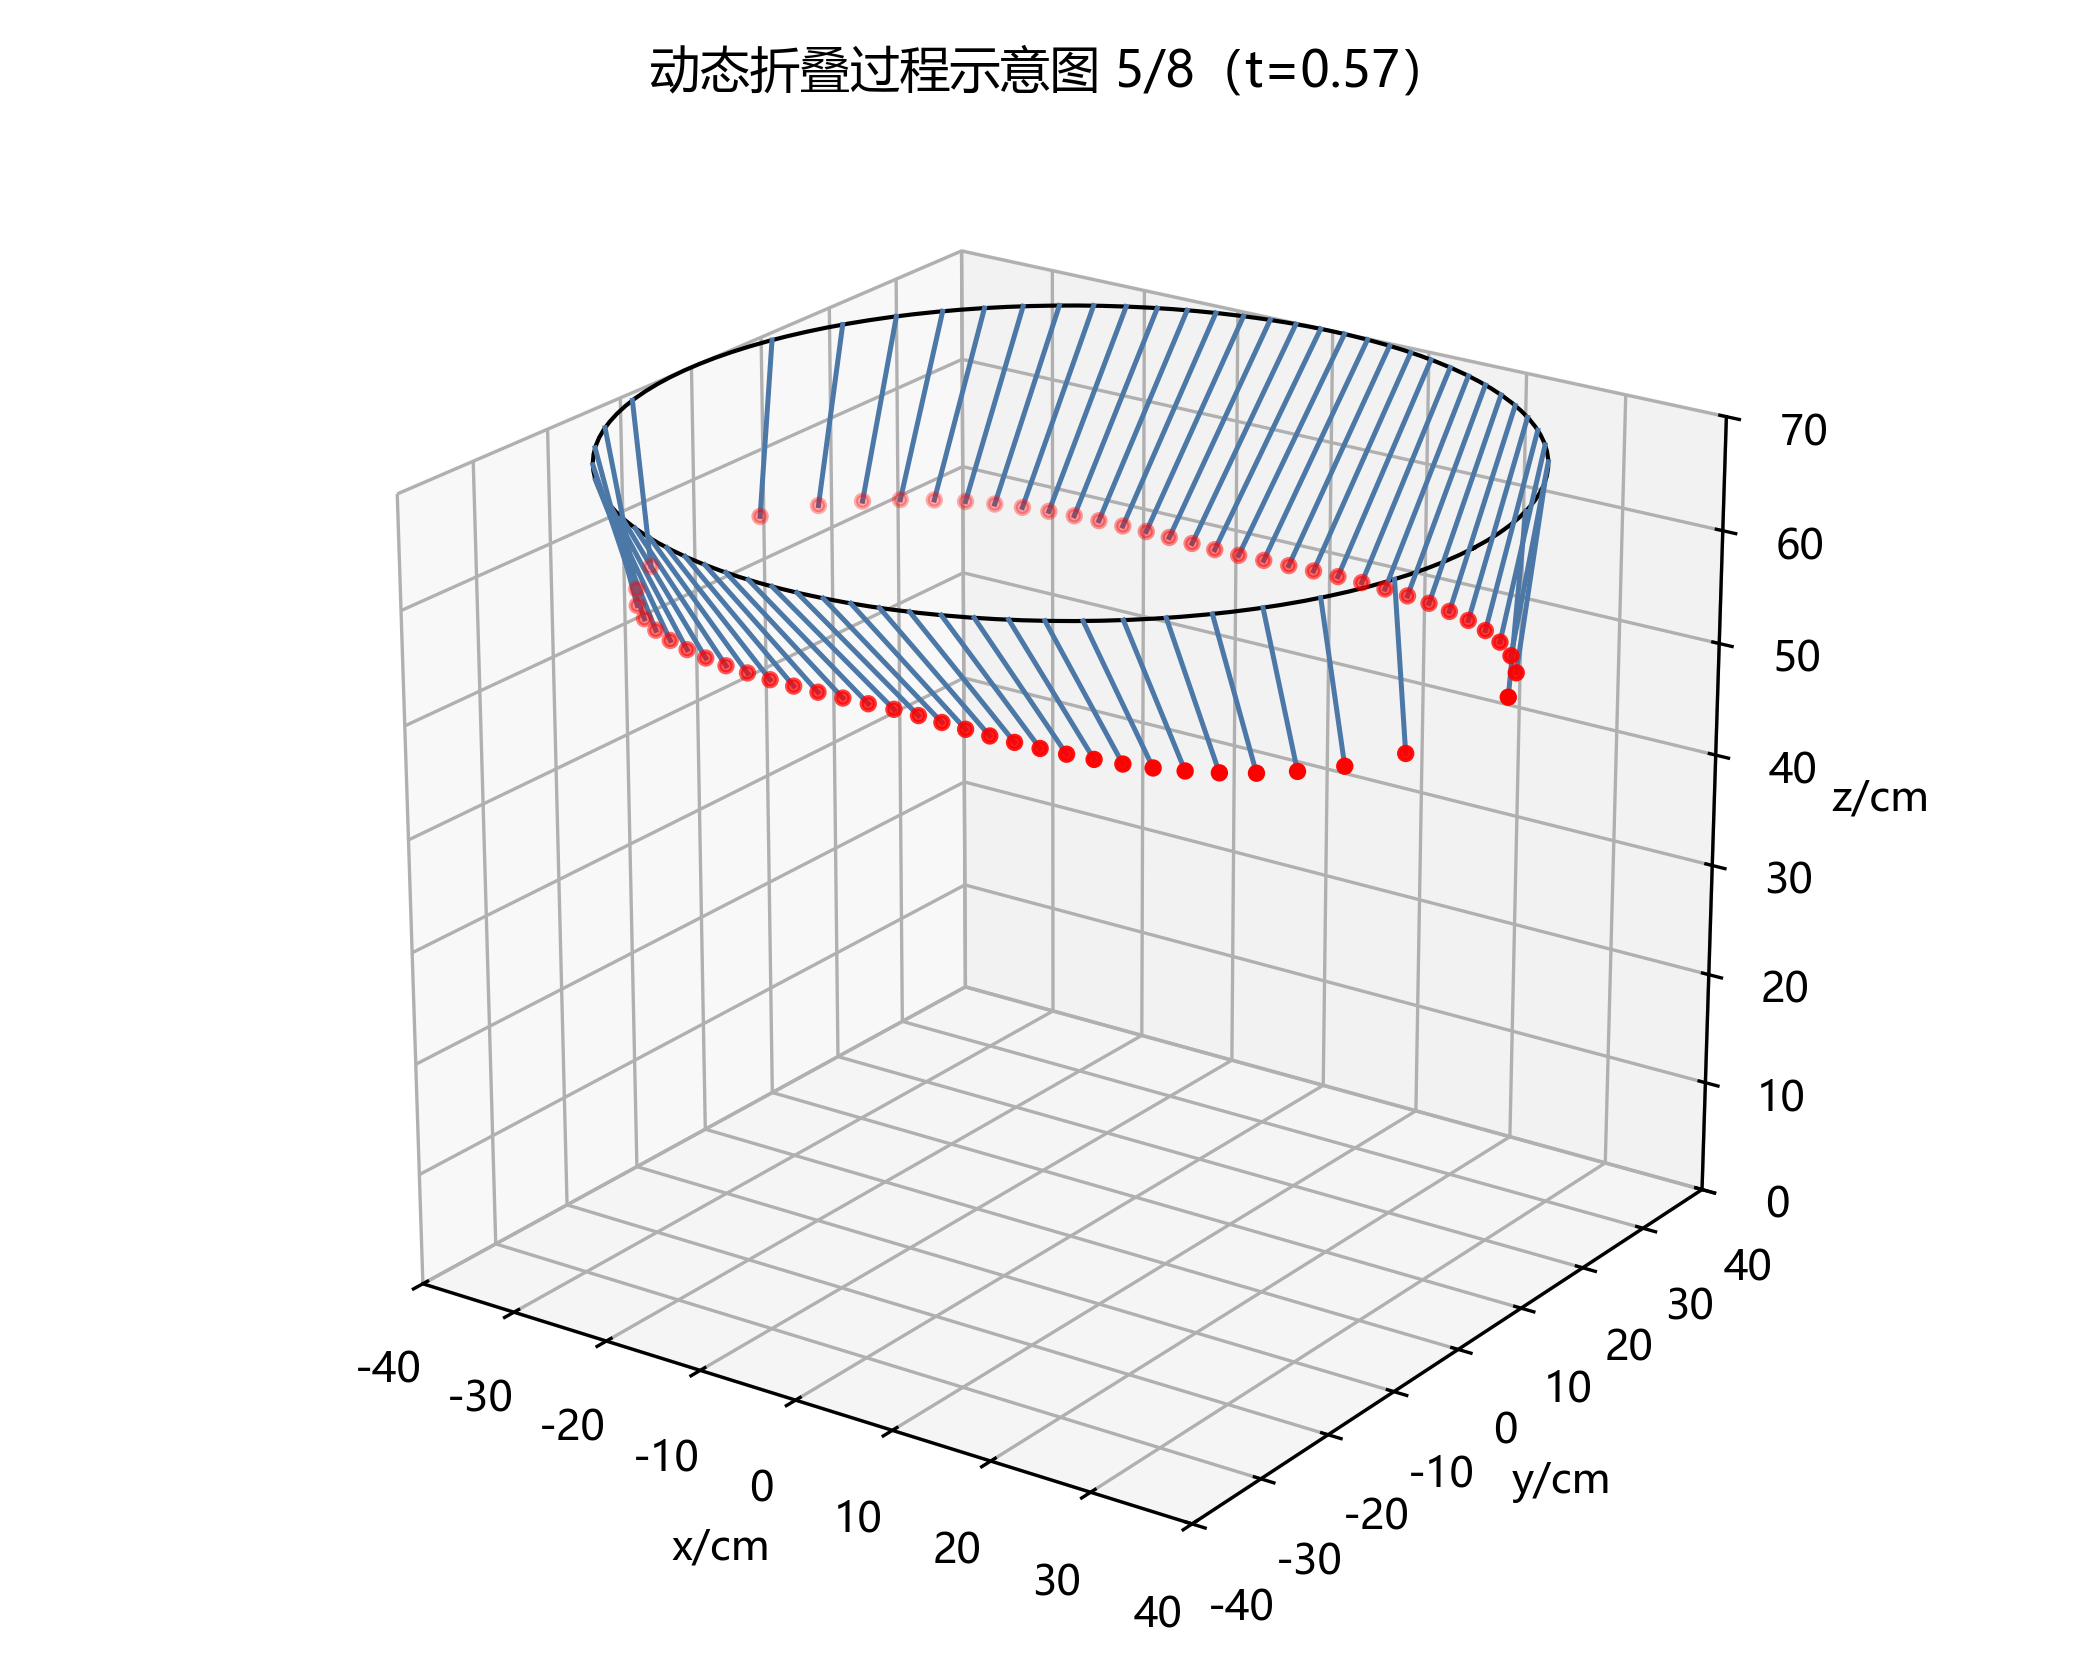
\includegraphics[width=\textwidth]{q3_software_dynamic_05.png}\caption{5}\end{subfigure}
\begin{subfigure}{0.24\textwidth}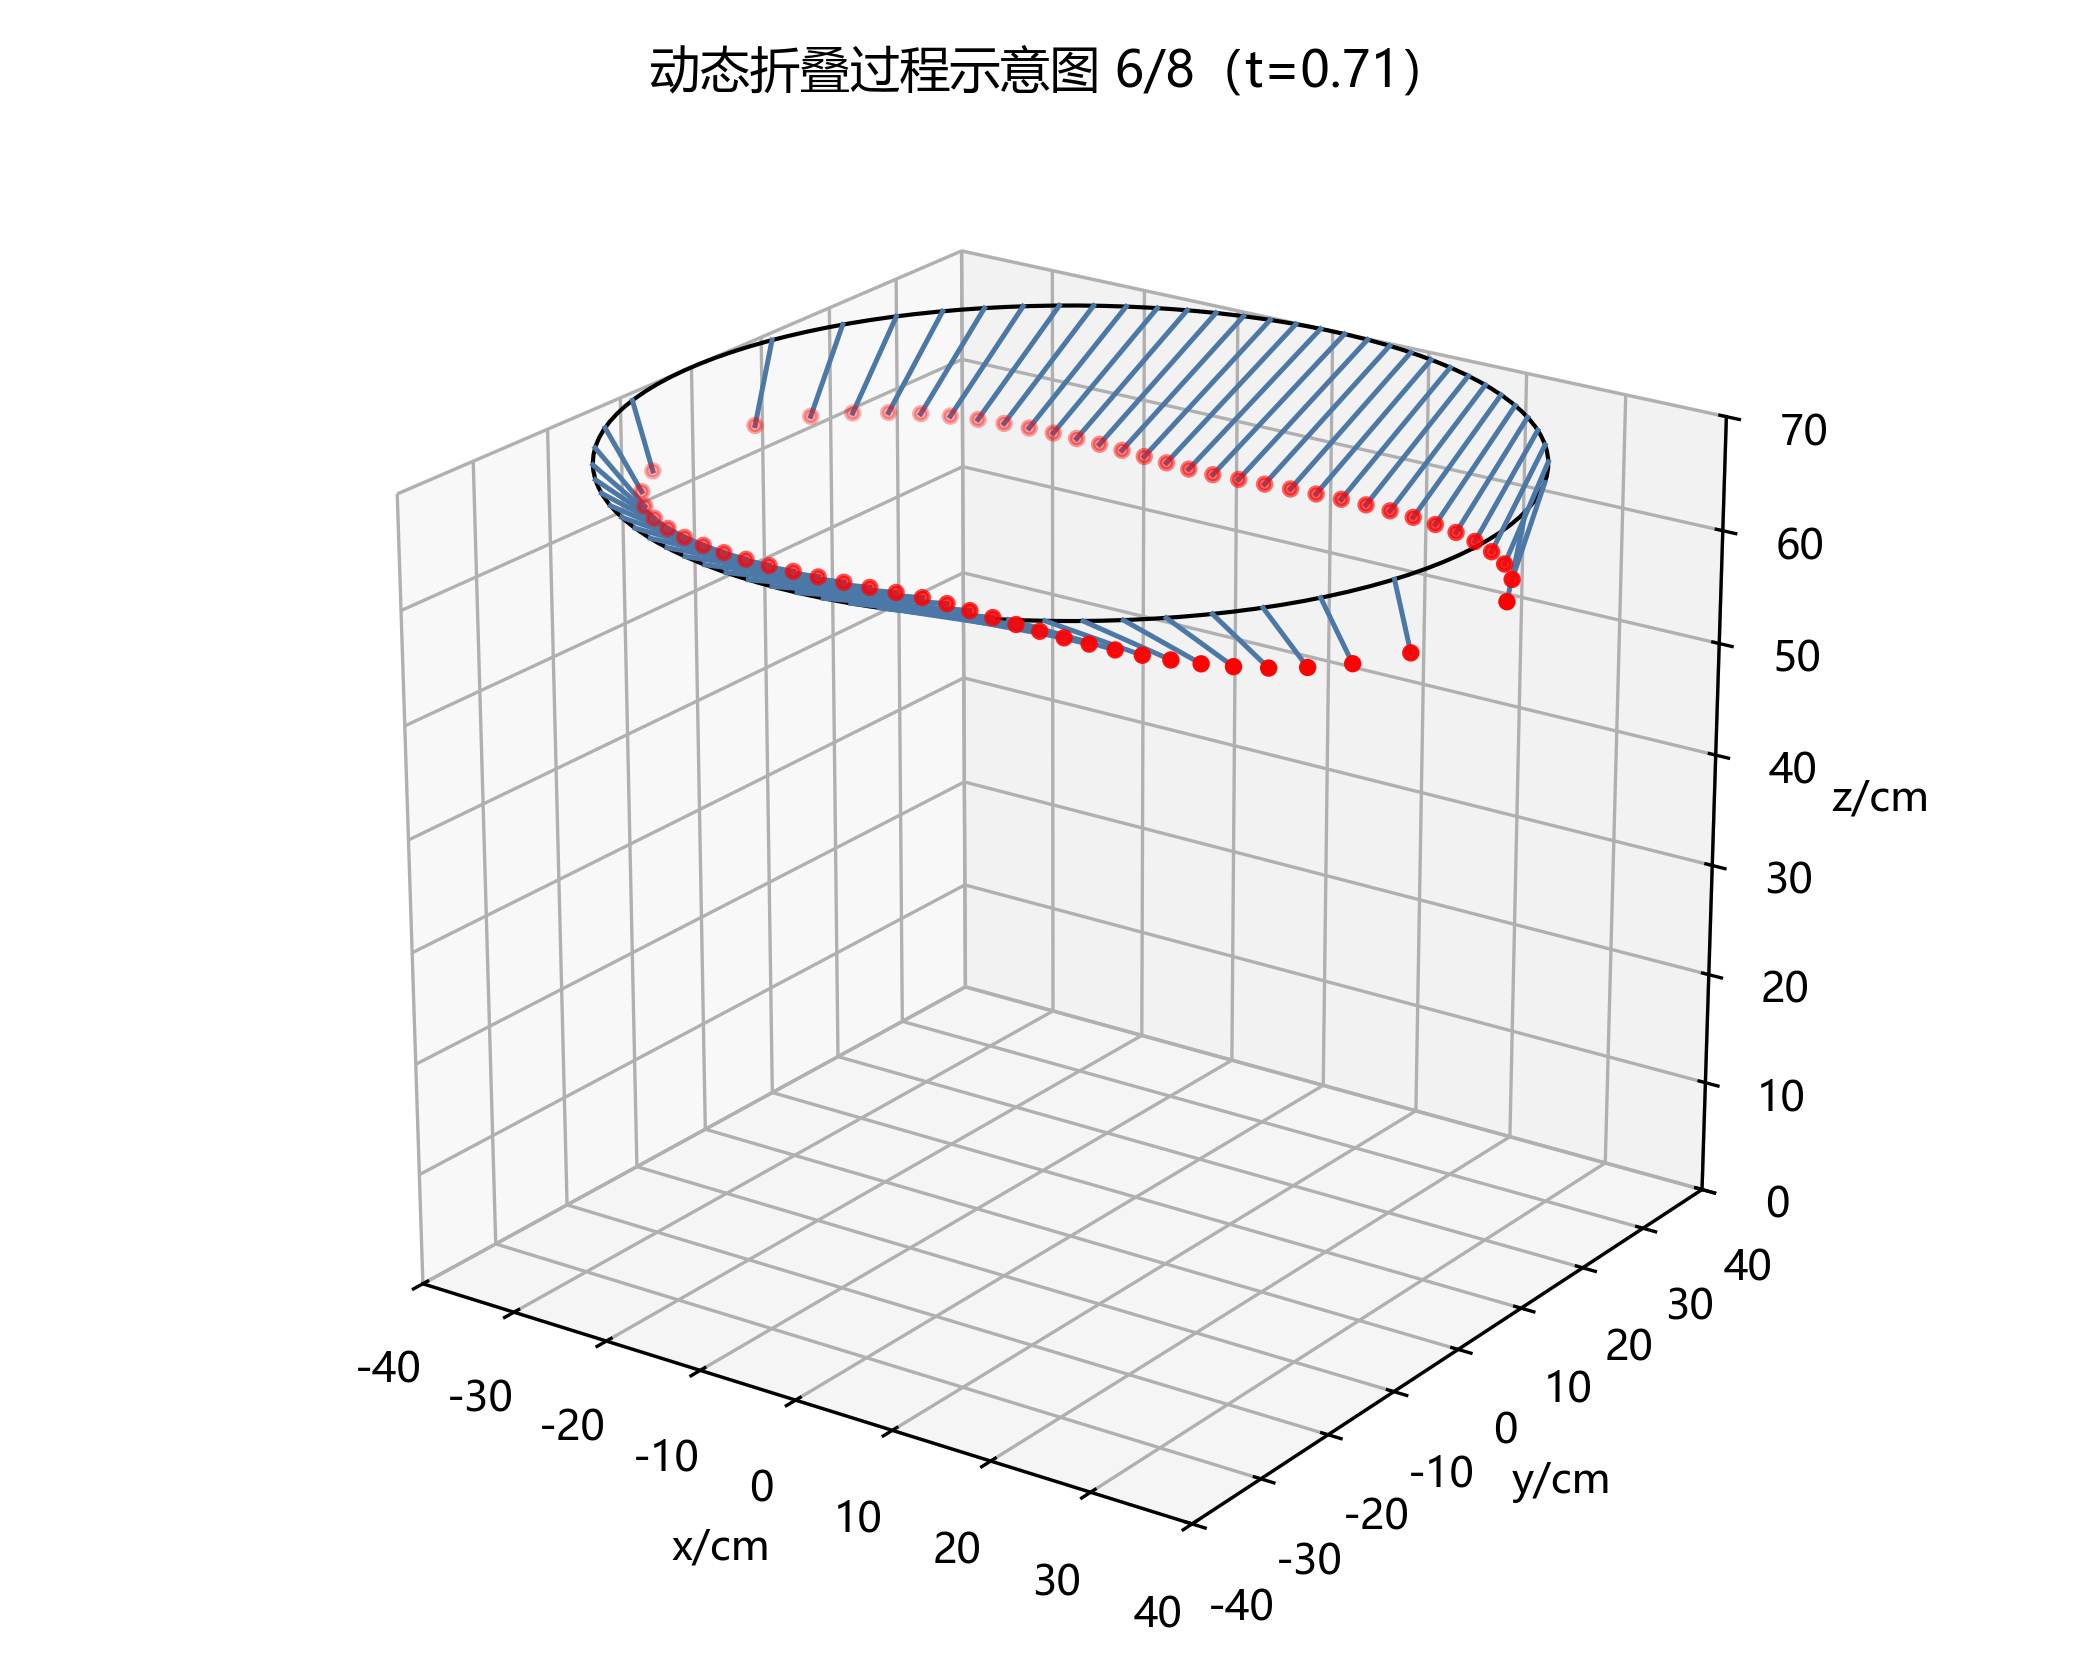
\includegraphics[width=\textwidth]{q3_software_dynamic_06.png}\caption{6}\end{subfigure}
\begin{subfigure}{0.24\textwidth}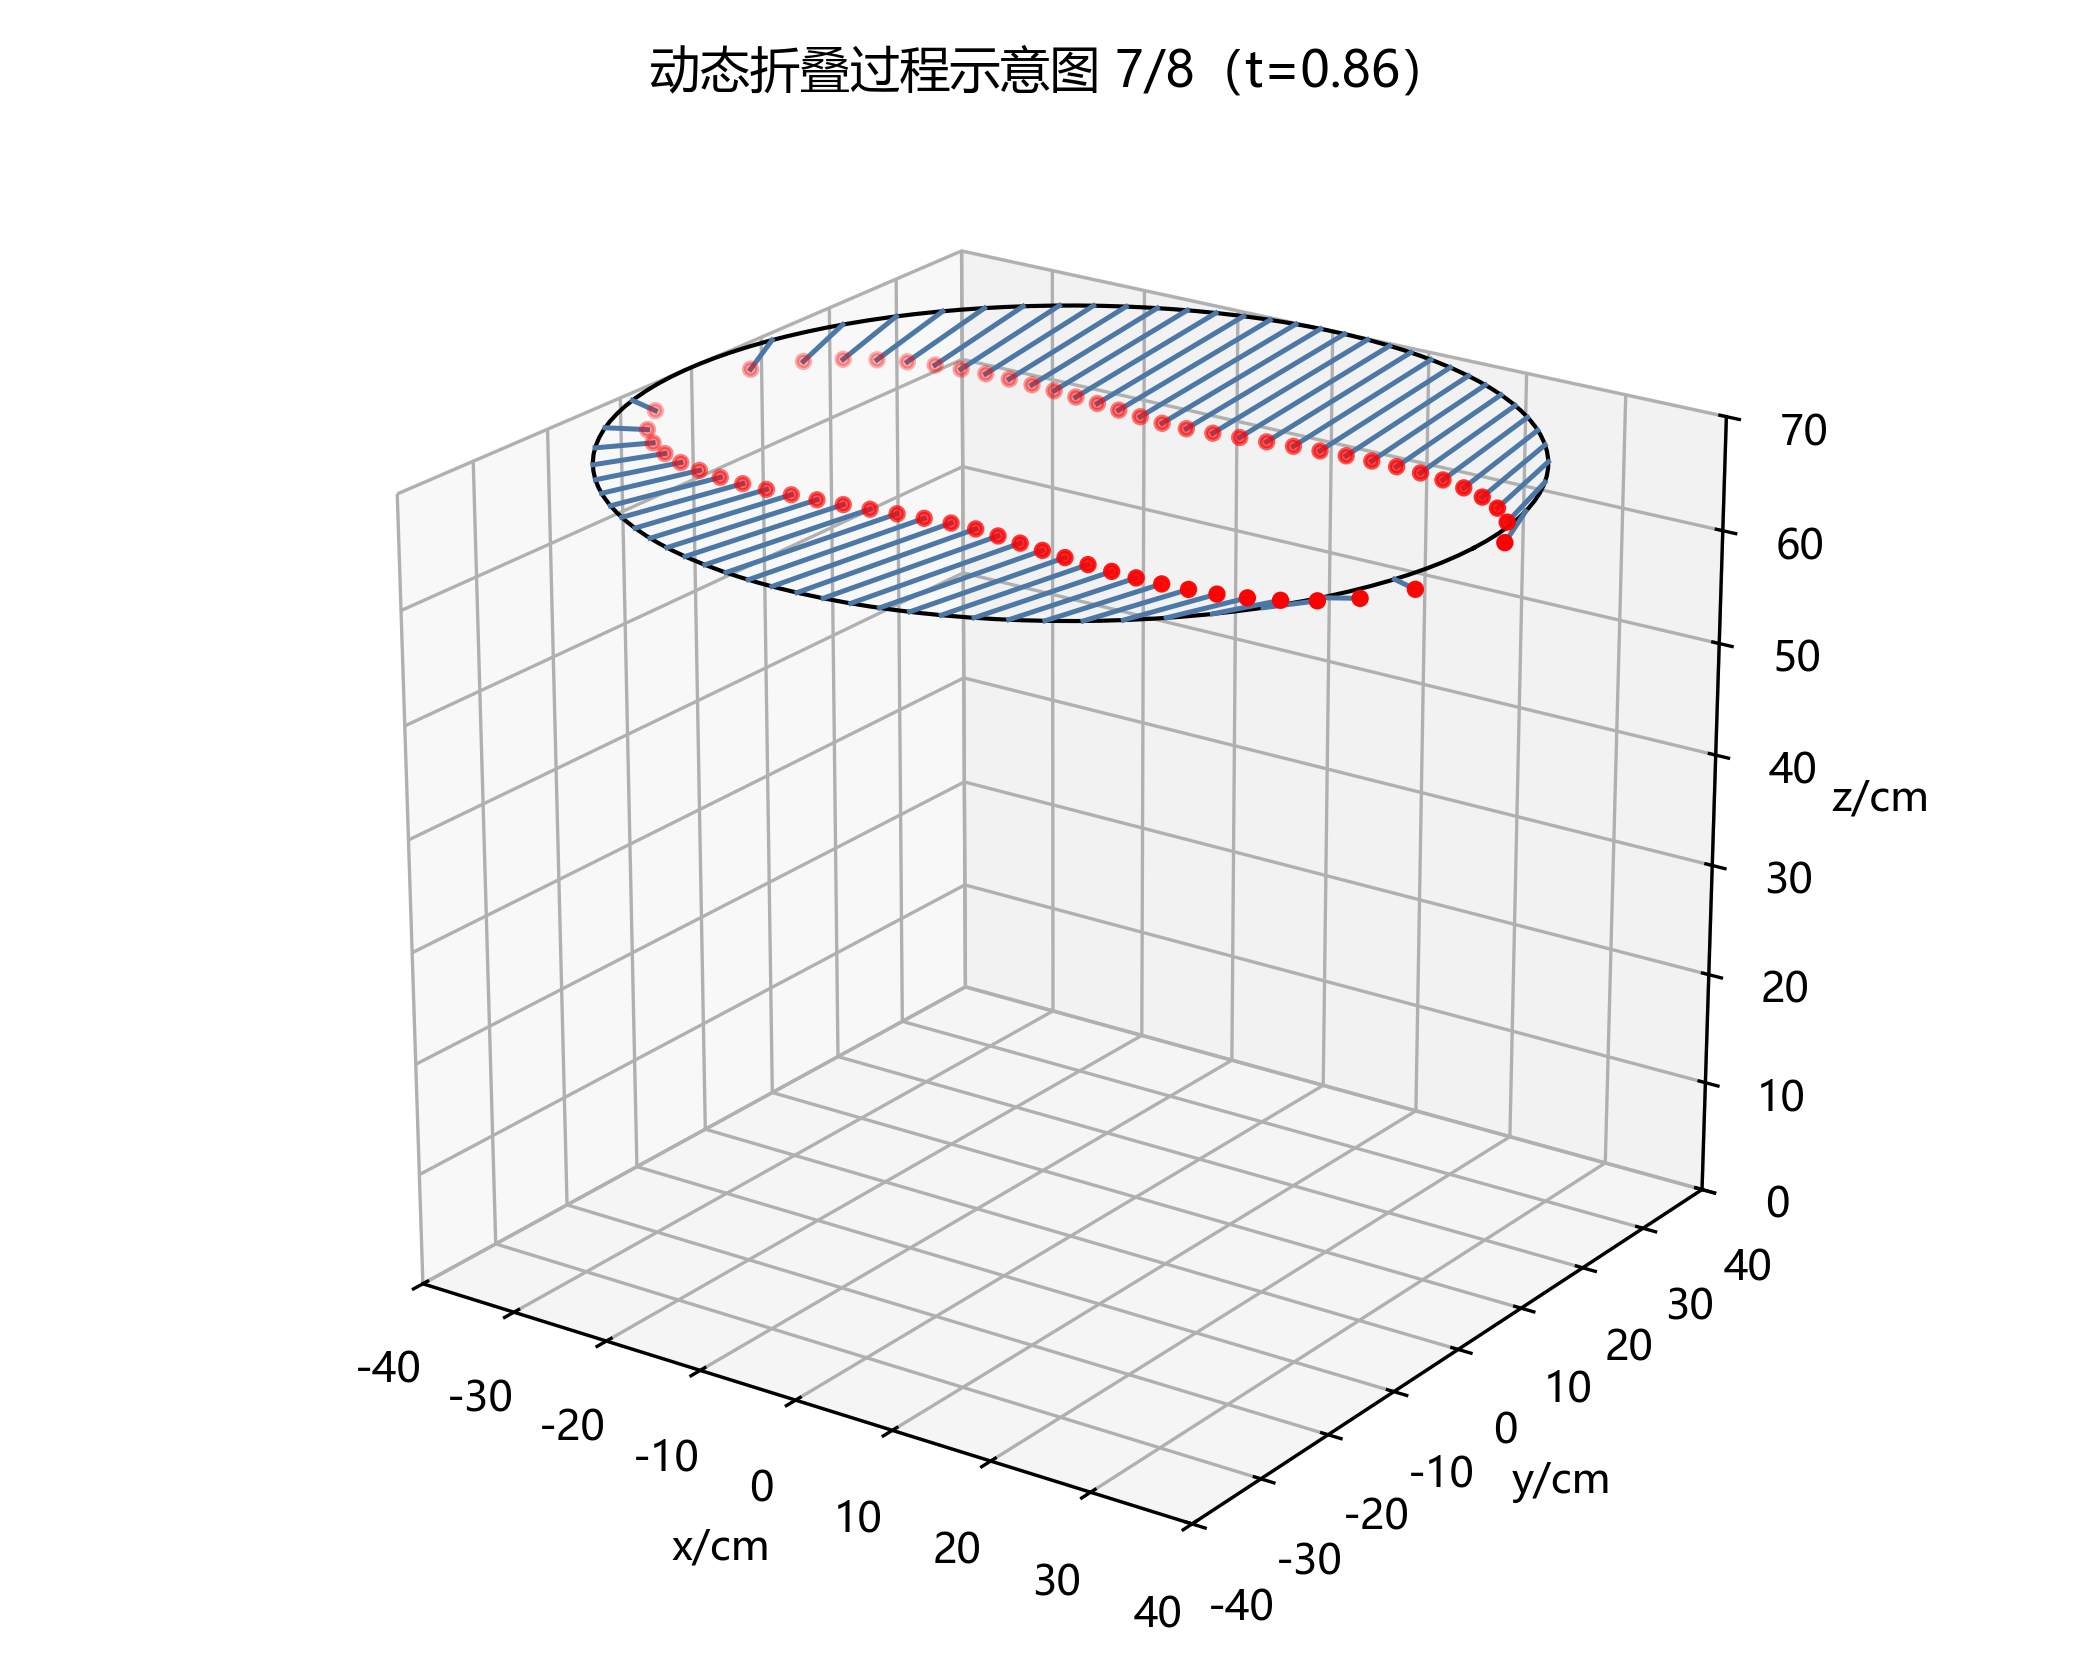
\includegraphics[width=\textwidth]{q3_software_dynamic_07.png}\caption{7}\end{subfigure}
\begin{subfigure}{0.24\textwidth}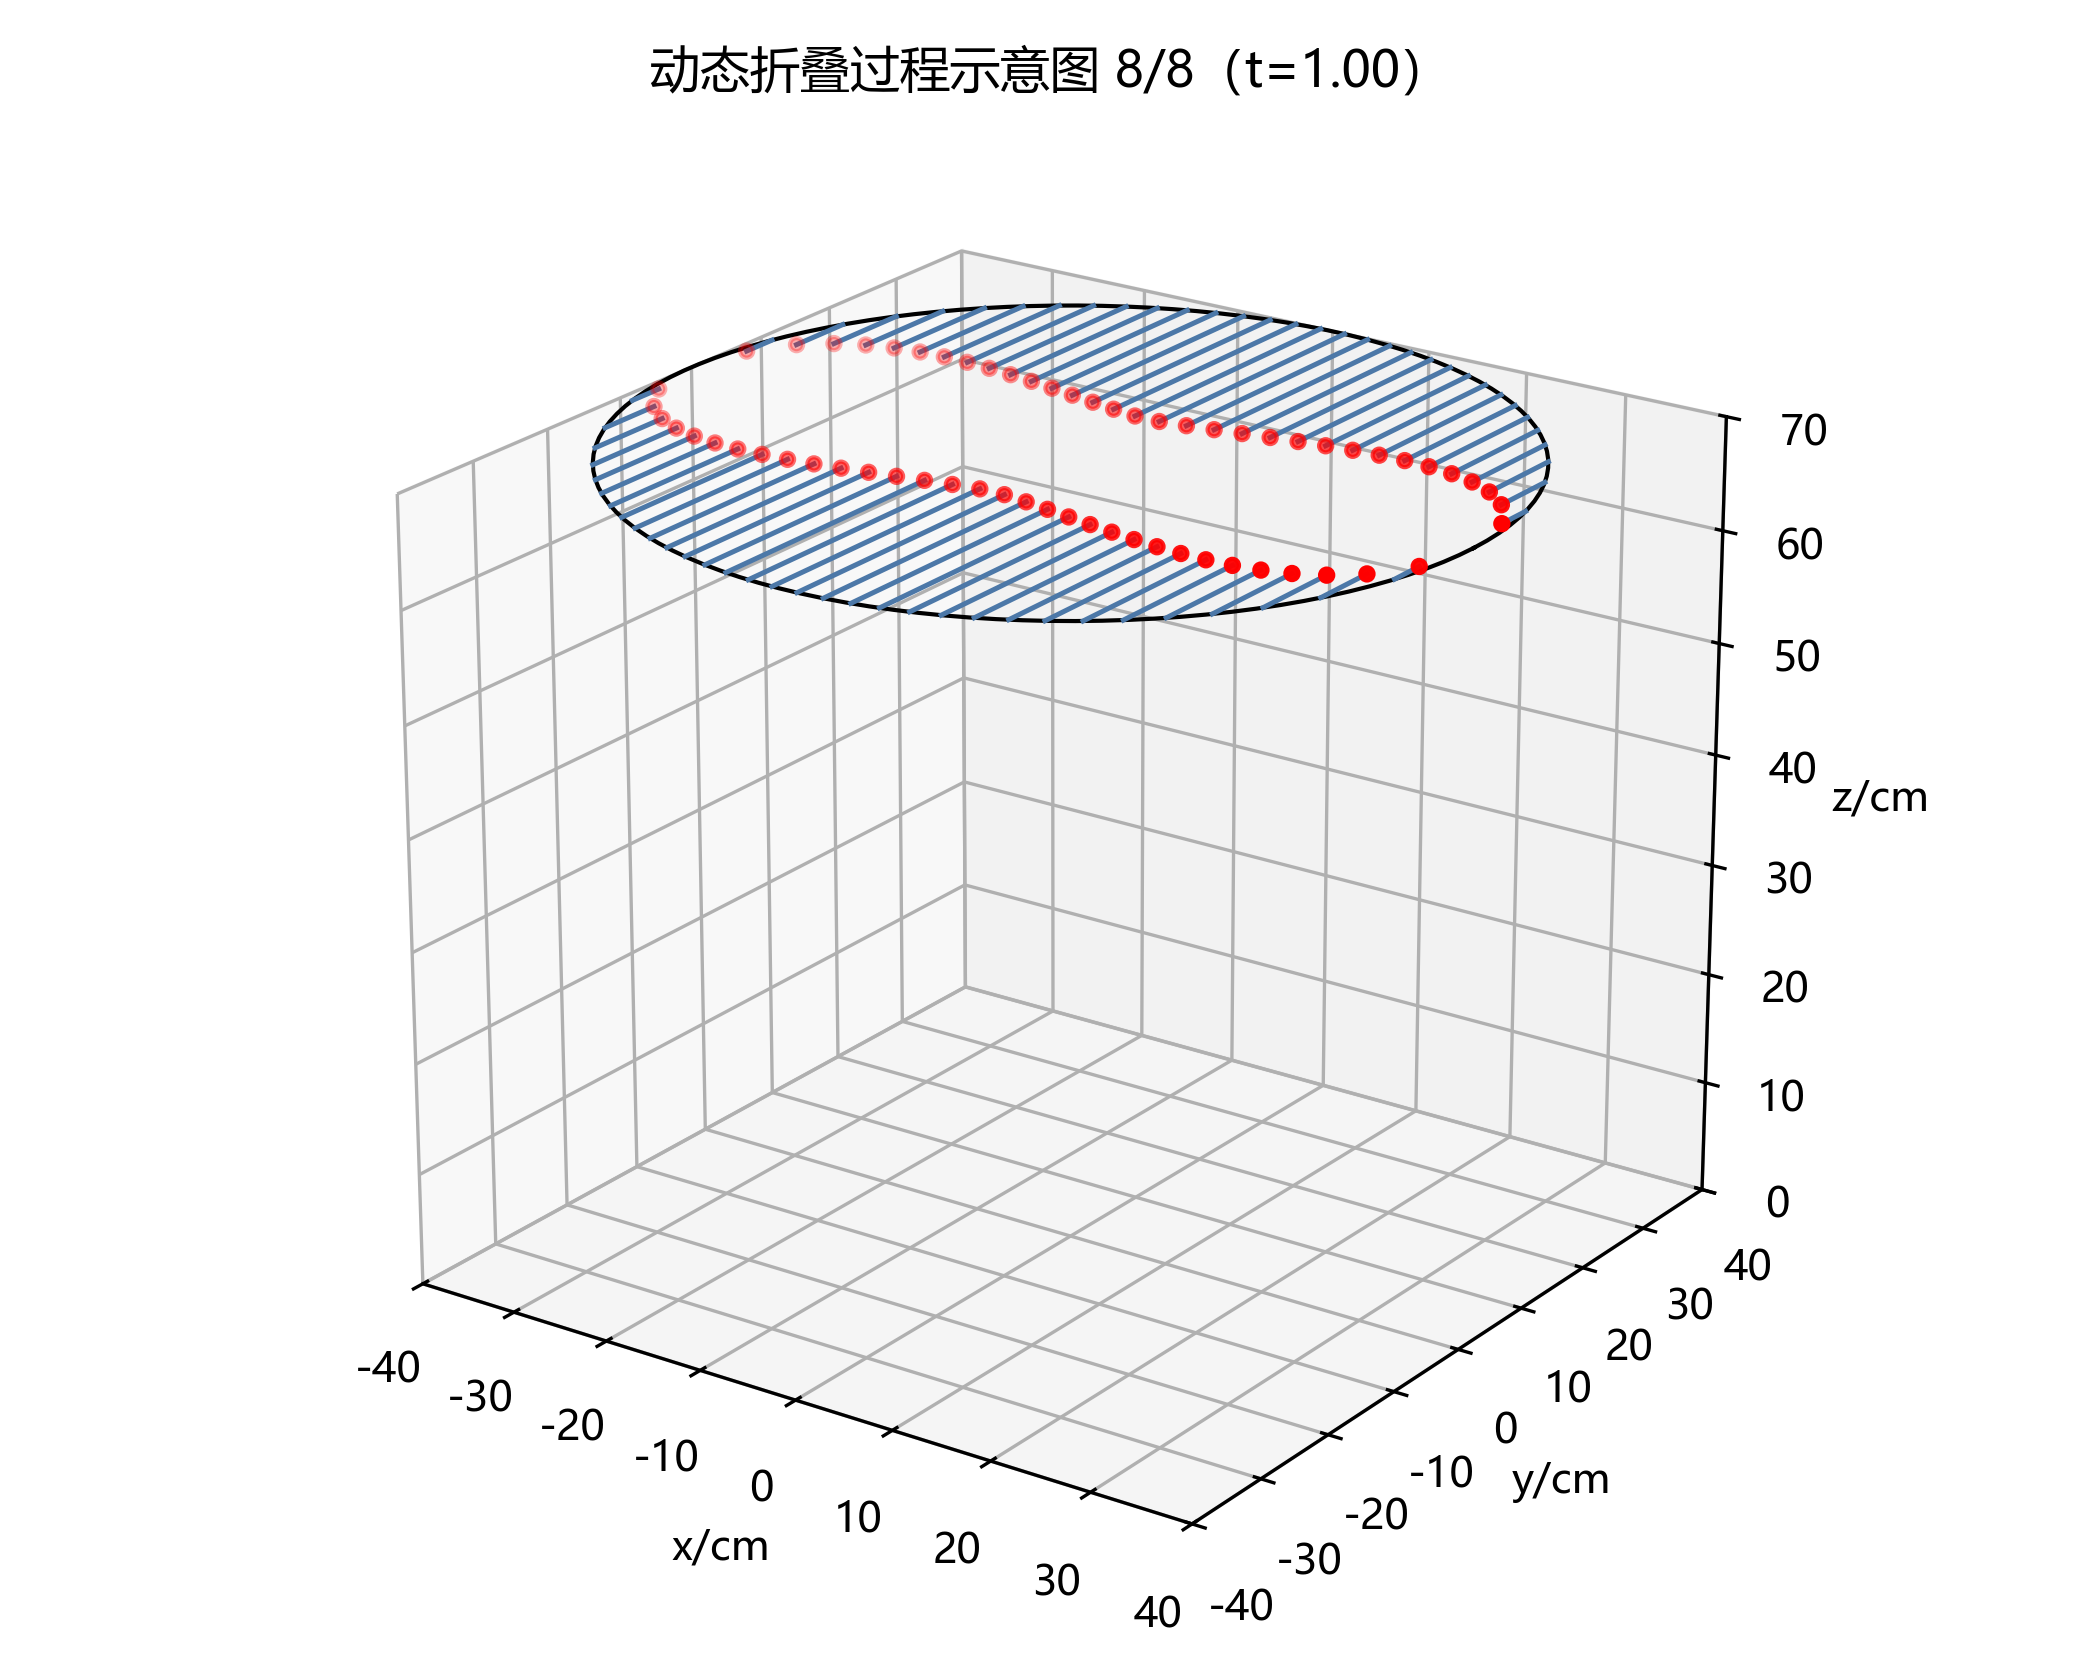
\includegraphics[width=\textwidth]{q3_software_dynamic_08.png}\caption{8}\end{subfigure}
\caption{设计软件输出的8张动态变化过程图}
\label{fig:q3dynamic}
\end{figure}
图\ref{fig:q3dynamic}满足题目“至少8张动态变化过程示意图”的要求。八个时刻从平摊到成桌连续变化，能够作为软件界面的动画预览帧。用户改变桌高或边界曲线后，只需重新计算离散端点和木条参数，即可生成新的动画帧。

\section{模型检验、对比与敏感性分析}
\subsection{约束满足检验}
本文对问题一和问题二的最终方案进行了几何约束检验。首先，所有木条长度均大于对应桌高，且由公式 $l_i=\sqrt{H^2+(y_i^t-y_i^f)^2}$ 计算得到，不存在长度不足。其次，所有桌脚点满足 $0\le y_i^f\le y_i^t$，即桌脚位于桌面投影内部。再次，问题二最大开槽长度 $2.773\cm$ 小于最大木条长度的18\%，满足加工约束。

对于稳定性，问题一支撑半径为 $24.254\cm$，占桌面半径的97.02\%；问题二支撑半径为 $39.251\cm$，占桌面半径的98.13\%。这说明桌脚边缘几乎覆盖桌面半径范围，在几何层面具有较好的抗倾覆潜力。由于本题未给出载荷和材料强度参数，本文没有进行力学应力检验，这一点在模型局限中说明。

\subsection{baseline 对比}
问题一的 baseline 是竖直或近竖直支撑模型，该模型虽能满足高度，但桌脚边缘线缺乏题图所示的曲面造型。本文模型通过式(3)给出连续桌脚边缘线，同时将最大开槽控制在 $2.315\cm$，实现了形状和加工性的平衡。

问题二的 baseline 是 $W=D=80\cm,\eta=0.5$。该 baseline 最大开槽长度为 $3.618\cm$，优化方案最大开槽长度为 $2.773\cm$，降低约23.36\%。稳定性指标从0.9161增至0.9173，变化不大；这说明在该实例中，优化的主要贡献是通过调整钢筋位置降低开槽加工难度，而不是牺牲稳定性去减少材料。

\subsection{敏感性分析}
本文对问题二最优方案的两个关键参数进行 $\pm15\%$ 单因素扰动：平板宽度 $W$ 和钢筋位置比例 $\eta$。每次扰动后重新计算稳定性和最大开槽长度。结果见图\ref{fig:q2sens}。

\begin{figure}[H]
\centering
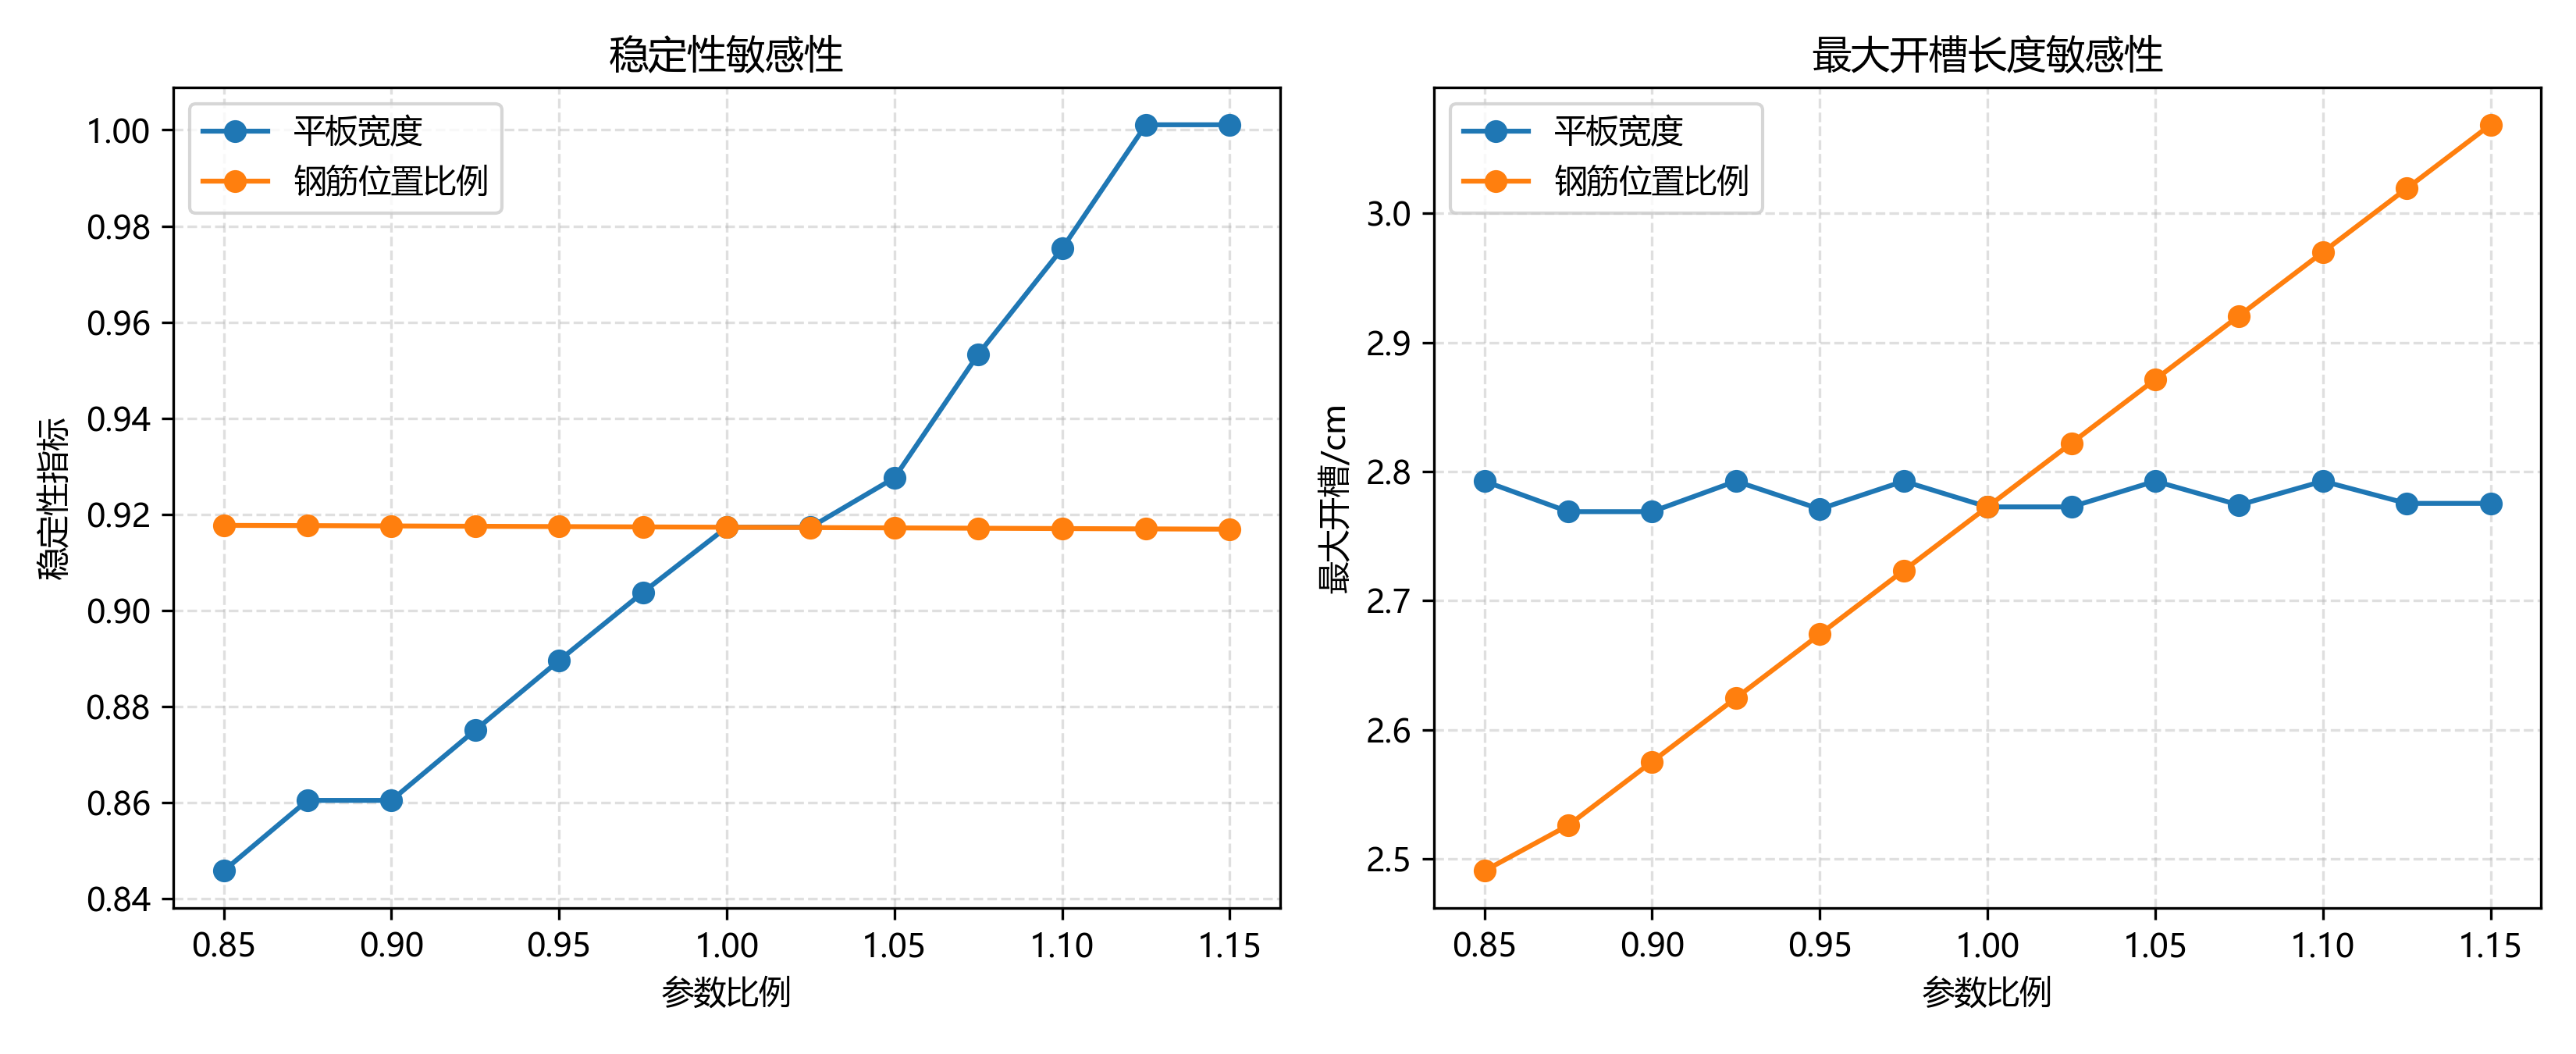
\includegraphics[width=0.86\textwidth]{q2_sensitivity.png}
\caption{问题二关键参数敏感性分析}
\label{fig:q2sens}
\end{figure}
由图\ref{fig:q2sens}可知，平板宽度变化主要影响稳定性，宽度增大时支撑范围扩大，稳定性提高；钢筋位置比例变化主要影响最大开槽长度，$\eta$ 越大，开槽越长。冻结数字显示，在 $\pm15\%$ 范围内，稳定性最大变化约16.93\%，最大开槽长度最大变化约20.84\%。因此，若实际生产中更重视加工便利性，应优先控制钢筋位置比例；若更重视抗倾覆能力，则可适当增加平板宽度或桌脚外缘比例。

\subsection{可复现性检验}
全部计算由 \texttt{code/main\_modeling.py} 完成，运行后自动生成结果表、图表和 \texttt{results/frozen\_numbers.json}。论文中的关键数字均来自该冻结文件。图表由 Matplotlib 以300 dpi 保存，没有使用人工改数。优化算法固定随机种子42，重复运行脚本可复现同一组核心结果。

\section{模型评价、改进与推广}
\subsection{模型优点}
\begin{enumerate}
\item \textbf{几何关系清晰。} 本文从桌面边界、桌脚边界和桌高出发，直接推导木条长度、倾角和开槽长度，变量含义明确，便于加工人员理解。
\item \textbf{能同时回答三个问题。} 问题一的固定尺寸设计、问题二的优化设计和问题三的软件化设计都使用同一套离散直纹曲面框架，模型具有一致性。
\item \textbf{加工参数可落地。} 输出不仅有外形图，还包含每根木条长度、开槽长度和钢筋孔位比例，可直接整理为加工表。
\item \textbf{可视化充分。} 模型生成了桌脚边缘线、参数分布、三维成型图和8张动态过程图，能直观验证折叠过程是否连续。
\end{enumerate}

\subsection{模型局限}
\begin{enumerate}
\item 本文主要进行几何与加工层面的建模，未建立完整的受力模型。实际产品仍需根据木材强度、连接件强度和载荷分布做结构校核。
\item 开槽长度采用几何投影近似，并加入加工余量，未精确模拟铰链、钢筋直径和槽宽之间的接触运动。
\item 稳定性指标是启发式综合指标，虽然能反映支撑半径、倾角和开槽复杂度，但不能替代真实倾覆实验。
\item 问题三的创意形状以参数曲线为例，若客户输入自由手绘曲线，还需要增加曲线平滑、碰撞检测和局部不可行修复。
\end{enumerate}

\subsection{改进方向}
后续可从三方面改进。第一，引入静力学模型，计算桌面受载时各木条轴力、铰链反力和钢筋剪力，并将最大应力作为优化约束。第二，使用多体机构仿真精确计算钢筋在槽内的轨迹，从而替代本文的投影近似开槽公式。第三，在设计软件中增加交互式权重调节和不可行形状提示，使用户能在美观、稳定和成本之间快速取舍。

\subsection{推广应用}
本文的离散直纹曲面建模方法不仅适用于折叠桌，也可推广到折叠凳、可展开展架、折叠屏风和临时展台等产品。凡是由多根平行条带通过铰链和滑槽形成空间支撑面的结构，都可以采用“边界离散--母线生成--加工参数计算--多目标优化”的流程进行快速设计。

\section{结论}
本文围绕2014B创意平板折叠桌建立了完整数学模型并给出可复现结果。主要结论如下：
\begin{enumerate}
\item 对给定 $120\cm\times50\cm\times3\cm$ 平板和 $53\cm$ 桌高，模型采用20根木条，有效平板尺寸为 $111.827\cm\times50.000\cm\times3\cm$，木条长度范围 $53.079$--$55.913\cm$，最大开槽 $2.315\cm$，桌脚边缘线由式(3)给出。
\item 对 $H=70\cm,D=80\cm$ 的优化设计，得到平板尺寸 $151.272\cm\times80.000\cm\times3\cm$，木条数32根，钢筋位置比例 $\eta=0.3500$，最大开槽 $2.773\cm$，稳定性指标0.9173。
\item 面向设计软件，本文提出了基于桌面边界和期望桌脚边界的通用优化模型，并给出椭圆、圆角方形和花瓣形三类创意桌方案，生成了满足题意的8张动态变化示意图。
\item 敏感性分析表明，在 $\pm15\%$ 参数扰动下，稳定性最大变化约16.93\%，最大开槽长度变化约20.84\%。模型对平板宽度和钢筋位置敏感，但敏感方向清楚，便于工程调参。
\end{enumerate}

\section*{参考文献}
\addcontentsline{toc}{section}{参考文献}
\begin{enumerate}[label={[\arabic*]}]
\item 姜启源, 谢金星, 叶俊. 数学模型[M]. 北京: 高等教育出版社, 2018.
\item 同济大学数学科学学院. 高等数学[M]. 北京: 高等教育出版社, 2014.
\item Nocedal J, Wright S J. Numerical Optimization[M]. New York: Springer, 2006.
\item Storn R, Price K. Differential Evolution--A Simple and Efficient Heuristic for Global Optimization over Continuous Spaces[J]. Journal of Global Optimization, 1997, 11: 341--359.
\item 全国大学生数学建模竞赛组委会. 全国大学生数学建模竞赛论文格式规范[EB/OL]. 2014.
\end{enumerate}

\appendix
\section{支撑材料说明}
支撑材料目录包括：\texttt{code/main\_modeling.py} 为主程序；\texttt{tables/} 存放各问题参数表；\texttt{quest1/figures/}、\texttt{quest2/figures/}、\texttt{quest3/figures/} 存放图表；\texttt{results/frozen\_numbers.json} 存放论文冻结数字；\texttt{references/} 存放题面提取和知识库检索记录。运行方式为在支撑材料目录执行：
\begin{verbatim}
python code/main_modeling.py
\end{verbatim}

\section{三层质量门控审计}
\begin{itemize}
\item L1建模合理性：通过。三个子问题均建立了题目要求到模型输出的映射，假设服务于刚体几何、对称性和加工参数计算，baseline 与主模型差异明确。
\item L2求解正确性：通过。代码固定随机种子，生成参数表、图表和冻结数字；几何约束、开槽约束和敏感性分析均已完成。
\item L3论文质量：通过。摘要包含所有子问题方法和关键数字，正文包含公式、图表解释、baseline 对比、敏感性分析、模型评价和支撑材料说明。
\end{itemize}

\end{document}
